% Remove the oneside option below for double sided printing (e.g. for final (post-viva) submission)
\documentclass[a4paper,12pt,oneside,openright]{book}

% Preamble commands go here
\usepackage{customisations}
\usepackage[Bjornstrup]{fncychap}
\usepackage{booktabs} 
\usepackage{amsmath} 
\usepackage{textcomp} 
\usepackage{xcolor}
\usepackage{slashed}
\usepackage{graphicx}
\usepackage{float}
\usepackage{afterpage}
\usepackage{amssymb}
\usepackage{multirow}
\usepackage{url}
\usepackage{float}
\usepackage{url}
\usepackage{tikz}
\usetikzlibrary{arrows}
\usepackage{tikz-3dplot}
\usepackage{enumitem}
\usepackage{tabularx}
\newcolumntype{C}[1]{>{\centering\arraybackslash}p{#1}}
\usepackage[compat=1.1.0]{tikz-feynhand}
\usepackage{tikz-feynman}
\tikzfeynmanset{compat=1.0.0}
\usepackage{simpler-wick}
%\usepackage{nopageno}


\usepackage{
  pgf,
  tikz}
\usetikzlibrary{
  arrows,
  trees,
  scopes,
  decorations.text,
  decorations.pathreplacing,
  decorations.pathmorphing,
  decorations.markings,
  positioning,
  calc,
  patterns,
  intersections,
  shapes,
  fadings
}

\usetikzlibrary{trees}
\usetikzlibrary{decorations.pathmorphing}
\usetikzlibrary{decorations.markings}

\tikzset{
  photon/.style=
  {
    decorate,
    decoration={snake},
    draw=black
  },
  particle/.style=
  {
    very thick,
    draw=black,
    postaction={decorate},
    decoration=
    {
      markings,
      mark=at position .5 with {\arrow[draw=black]{>}}
    }
  },
  antiparticle/.style=
  {
    very thick,
    draw=black,
    postaction={decorate},
    decoration=
    {
      markings,
      mark=at position .5 with {\arrow[draw=black]{<}}
    }
  },
  gluon/.style=
  {
    decorate,
    draw=black,
    decoration=
    {coil,
      amplitude=4pt,
      segment length=5pt
    }
  },
  scalar/.style=
  {
    densely dashed,
    draw=black
  }
 }

% \tikzset{
%   ch_scalar/.style=
%   {
%     densely dashed,
%     thick,
%     draw=mLightBrown,
%     postaction={decorate},
%     decoration=
%     {
%       markings,
%       mark=at position .6 with {\arrow[thick,draw=black]{>}}
%     }
%   },
%   majorana/.style=
%   {
%     draw=mLightBrown
%   },
%   posit/.style=
%   {
%     rectangle,
%     outer sep=0,
%     inner sep=0,
%   },
%   dirac/.style=
%   {
%     draw=mLightBrown,
%     postaction={decorate},
%     decoration=
%     % {
%     %   markings,
%     %   mark=at position .6 with {\arrow[thick,draw=black]{>}}
%     % }
%   },
%   vector/.style=
%   {
%     draw=mLightBrown,
%     decorate,
%     decoration={snake,amplitude=1.5pt,segment length=3pt}
%   },
%   rev_dirac/.style=
%   {
%     draw=mLightBrown,
%     postaction={decorate},
%     decoration=
%     {
%       markings,
%       mark=at position .6 with {\arrow[thick,draw=black]{<}}
%     }
%   },
%   me_quark/.style=
%   {
%     draw=mLightBrown,
%     line width=0.6
%   },
%   ps_quark/.style=
%   {
%     draw=black
%   },
%   scalar/.style=
%   {
%     densely dashed,
%     thick,
%     draw=black,
%   },
%   gluon/.style=
%   {
%     decorate,
%     draw=black,
%     line width=0.6,
%     decoration={coil,amplitude=1.8,segment length=2}
%   },
%   me_gluon/.style=
%   {
%     decorate,
%     draw=mLightBrown,
%     line width=0.6,
%     decoration={coil,amplitude=1.8,segment length=2}
%   },
%   ps_gluon/.style=
%   {
%     decorate,
%     draw=black,
%     decoration={coil,amplitude=1.8,segment length=2}
%   },
%   mi_gluon/.style=
%   {
%     decorate,
%     draw=black,
%     decoration={coil,amplitude=1.8,segment length=2}
%   },
%   mi_quark/.style=
%   {
%     fill=black,
%   },
%   pdf_line/.style=
%   {
%     draw=\pdfcol,
%     double,
%   },
%   ps_blob/.style=
%   {
%     circle,
%     draw=black,
%     fill=black,
%     inner sep=0,
%     outer sep=0.5,
%     minimum size=1
%   },
%   pdf_blob/.style=
%   {
%     circle,
%     outer color=transparent!70,
%     inner color=transparent!20,
%     inner sep=1,
%     outer sep=0,
%     text=mLightBrown,
%   },
%   vertex/.style=
%   {
%     anchor=center,
%     circle,
%     draw=black,
%     fill=black,
%     inner sep=0,
%     outer sep=0.5,
%     minimum size=1
%   }
% }

% \makeatletter
% \def\parsecomma#1,#2\endparsecomma{\def\page@x{#1}\def\page@y{#2}}
% \tikzdeclarecoordinatesystem{page}{
%     \parsecomma#1\endparsecomma
%     \pgfpointanchor{current page}{north east}
%     % Save the upper right corner
%     \pgf@xc=\pgf@x%
%     \pgf@yc=\pgf@y%
%     % save the lower left corner
%     \pgfpointanchor{current page}{south west}
%     \pgf@xb=\pgf@x%
%     \pgf@yb=\pgf@y%
%     % Transform to the correct placement
%     \pgfmathparse{(\pgf@xc-\pgf@xb)/2.*\page@x+(\pgf@xc+\pgf@xb)/2.}
%     \expandafter\pgf@x\expandafter=\pgfmathresult pt
%     \pgfmathparse{(\pgf@yc-\pgf@yb)/2.*\page@y+(\pgf@yc+\pgf@yb)/2.}
%     \expandafter\pgf@y\expandafter=\pgfmathresult pt
% }
% \makeatother
% % For every picture that defines or uses external nodes, you'll have
% % to apply the 'remember picture' style. To avoid some typing, we'll
% % apply the style to all pictures.
% \tikzstyle{every picture}+=[remember picture, overlay]

% % By default all math in TikZ nodes are set in inline mode. Change this to
% % displaystyle so that we don't get small fractions.
% %\everymath{\displaystyle}

% %\tikzstyle{na} = [baseline=-.5ex]

% \definecolor{mLightBrown}{HTML}{EB811B}

%%% Local Variables: 
%%% mode: latex
%%% TeX-master: "bbh-intrinsic"
%%% End: 



\graphicspath{{./chapter2/figs/}{./chapter3/figs/}{./chapter4/figs/}{./chapter5/figs/}{./chapter6/figs/}{./chapter8/figs/}{./chapter9/figs/}}

\newcommand{\comment}[1]{\textbf{\textcolor{red!90!black}{[#1]}}}
\newcommand{\lp}{\left(}
\newcommand{\rp}{\right)}
\newcommand{\bare}{{(0)}}
\newcommand{\sym}{\mathrm{sym}}
\newcommand{\asy}{\mathrm{asy}}
\newcommand{\as}{\alpha_s}
\newcommand{\nsv}{\mathrm{V}_3}
\newcommand{\nst}{\mathrm{T}_3}
\newcommand{\eg}{{\em e.g.}}
\newcommand{\ie}{{\em i.e.}}
\newcommand{\dd}{{\rm d}}
\newcommand{\order}[1]{{\cal O}(#1)}
\newcommand{\msbar}{$\overline{\mathrm{MS}}$}  
\newcommand{\MSb}{\overline{\mathrm{MS}}}
\newcommand{\MMSb}{{\rm M}\overline{\mathrm{MS}}} 
\def \z{\zeta}
\newcommand\myemptypage{
    \null
    \thispagestyle{empty}
    \addtocounter{page}{-1}
    \newpage
}
\def\blankpage{%
    \clearpage%
    \thispagestyle{empty}%
    %\addtocounter{page}{-1}%
    \null%
    \clearpage
}

\title{Towards a new generation of Parton Distribution Functions: from high-precision collider data to lattice
Quantum Chromodynamics }
\author{Tommaso Giani}
\date{April 2021} % of submission

\begin{document}

% Thesis front matter - title page, abstract, acknowledgements, declaration and table of contents
% See customisations.sty to modify the title page or declaration
\singlespacing
\maketitlepage
\eighteenptleading
\frontmatter

For each chapter write smt like this.. 


The data presented in this thesis was obtained in an experiment carried out by the
[name of collaboration] in [location of experiment/where collaboration happened]. I
played a major role in the preparation and execution of the experiment, and the data
analysis and interpretation are entirely by own work. Any contributions from
colleagues in the collaboration, such as diagrams or calibrations, are explicitly
referenced in the text.
I am aware of and understand the university’s policy on plagiarism and I certify that
this thesis is my own work, expect where indicated by referencing, and the work
presented in it has not been submitted in support of another degree or qualification
from this or any other university or institute of learning. 
\chapter*{Lay Summary}
In this thesis we present a number of studies concerning the determination of the
Parton Distribution Functions (PDFs) of the proton. These results are important to gain a better understanding 
of the fundamental structure of the proton and are necessary to perform a number of relevant computations
in high energy-physics phenomenology.
Additionally, a precise knowledge of PDFs is likely to be a key ingredients for new physics studies. 
It is therefore important to produce more and more precise PDFs,
researching into new numerical frameworks and physical ideas. 
In this thesis we present a number of steps in this direction, addressing a number of different topics,
which span from the inclusion of new experimental data to recent developments from the lattice community.



\chapter*{Abstract}
A precise understanding of the proton structure, encoded in Parton Distribution Functions (PDFs), is required 
to make reliable predictions and analyses at the Large Hadron Collider (LHC), 
the main source of experimental data probing subnuclear interactions we have today.
PDFs have played a central role in the recent 
discovery of the Higgs boson and, since it is increasingly clear that any effect due to new physics 
will manifest itself as small deviations from the current theory, 
a precise determination of PDFs is likely to be a key ingredient 
for new physics studies.
%
The PDFs are formally defined as matrix elements of renormalized operators in Quantum Chromodynamics (QCD) involving hadronic states.
They are inherently non-perturbative quantities, and they are extracted from global QCD analysis over
experimental data using the so-called factorization theorems. 
Producing a new generation of PDFs, satisfying the precision and reliability requirements demanded by the current research,
is a challenging task which involves, together with the experimental data input, the development of robust
fitting methodologies, along with new physical ideas. 
%
In this thesis I present a number of progresses which have been developed in the last few years in the context of 
PDFs determination, some of which will lead to the next PDFs release by the NNPDF collaboration. 
In particular I will discuss a new framework for global PDFs determinations, the impact of new experimental data,
with particular emphasis on jets data, the inclusion of theory uncertainty in a PDFs fit 
and the treatment of heavy quarks distributions.
%
I will then discuss a set of recent ideas which would allow to extract PDFs from equal time correlators computable 
within the framework of lattice QCD, and I will present results regarding data coming from different 
lattice approaches and collaborations.

\blankpage



\cleardoublepage
\vspace*{\stretch{1}}
{\itshape A tutti i miei nonni
e a Franco Sar}
\vspace{\stretch{2}}
\cleardoublepage

\chapter*{Acknowledgments}
%
First of all, I would like to thank my supervisor, Luigi Del Debbio.
I am deeply happy and grateful for the work done together.
It has been stimulating, inspiring, exciting and extremely fun, and it has allowed me to grow up
quite a lot.
I truly consider our long blackboard discussions the most valuable thing of the whole PhD experience, and
I am looking forward for more of that in the coming years.
%
I am grateful to Stefano Forte, for the guide and help he has provided me, for the work done together 
and for always giving a complete answer to any question, usually in less than three minutes.
I would like to thank all the members of the particle theory group in Edinburgh, for the 
great and stimulating environment they have created, in particular Einan Gardi, Roman Zwicky and Richard Ball. 
%
I thank all the members of the NNPDF collaboration, with whom I have been working a lot during the last
few years. In particular I am deeply in debts with Emanuele R. Nocera, who has helped me a countless amount of 
times in a number of different tasks and projects, providing me with an example of efficiency, hard work and human kindness which
is difficult to match. I am grateful to Juan Rojo, for the support and the opportunity he gave me to work in his group
at the end of my PhD.
%
A special thank goes to Rabah, Cameron, Rosalyn, Michael, Zahari, Stefano, Shayan, Emma
and Luca. I have learnt a lot from each of them, in terms of physics, coding and teamwork, and it has been a real pleasure
to regularly meet them in the different meetings we had during the years.
In particular I want to thank Rosalyn and Michael for having shared with me the experience of being PhD students in Edinburgh.
It has been great for me to regularly see and work with them and I am grateful for all the trips
we had together around the world. 
I am also very proud of the progresses Michael has done in learning the basics of the italian language.
%
I want to thank Simone Marzani for the help and support he gave me, Marco Bonvini and Rhorry Gauld, for 
useful and stimulating discussions about resummation.  
%
I am grateful to Nathan P. Hartland for the many questions he answered, to
Davide Napoletano for the work done together and for the important help he provided me during the very first days of my PhD.
I want to thank Guido Cossu and Ava Khamseh for the work done together during my first year
and Anatoly Radyushkin for illuminating discussions, which allowed me to better understand the relation 
between light-cone and euclidean quantities. Finally, I would like to thank the master students who, when 
in person teaching was only partially allowed, regularly came to the QFT tutorials, watching me missing
minus signs and factors two at the blackboard.
Their interest, enthusiasm and questions have been of great support for me, and I have learnt a lot from them. 

%%
A number of not-physics friends have played a central role for me during my time in Edinburgh,
making me feel home every single day. It wouldn't have been possible for me to do any work without them.
% 
A huge thank you to Stefano, for a number of things which wouldn't fit a page. For the pizza, pasta al pesto,
creative swearwords and one-arm pull up sessions among other things. 
But, most of all, for being the best possible flatmate on earth.
I am pretty sure that without him I would have already died in some stupid way. 
%
I thank Lauren, for having helped me in a number of different ways, for her kindness, her support and for always being there,
during both the good and not-so-good times.  
I thank Roxane for the great time together, for the cycling, for having shown me parts of Scotland 
I had not seen before and for her help and support in looking for a job. 
%
A special thank you to my main British climbing buddies Ed and Patrick with whom I spent countless days and nights
pulling on tiny nasty crimps, dishonest slopers and silly pinches, discussing quality climbing videos.
And of course huge thanks to the whole Garage Crimpers team,
Scott, Colin and Sinclair. I am grateful for the countless sessions on the A2, on the 45.8 in the power garage 
and of course in the County, which, together with Dumby, has now a very special place among the longlist of my
favourite climbing spots. 
%
Thanks to Andrea, for having being close during a strange time, when the pandemic started.
Finally, I would like to thank Michael, who offered me a room during my very first days in Scotland, without even knowing 
who I was.

%   
I want to thank a number of friends from Italy, who have constantly supported and helped me in different ways.
Huge thanks to Gi, for having shared with me the first years of this experience and for having always being there for me,
despite everything.
Thanks to my serious dottorandi friends Fabbri, Tommy, Mario and Anna who in one way or another are always there.
I am always looking forward for seeing them every time we are all back to Italy (especially when this happens at Silvi).
Thanks to Alice, for the help and support provided during the last months of my PhD. 
Thanks to Rick, for the chats we have every time we see each other.
Huge thanks to Lollo, for being a beast, for all the climbing we are always having together every time
I am back to Italy and for the support he is always giving me.
Thanks to Ale, for the countless routes tried together and for always taking every single whipper.
Thanks to my Passaggio Obbligato friends, in particular to Fede Montagna and Teo Nill, who 
regularly sent me supportive messages. 
Finally thanks to Luca, who in his own way has always been there for me.

Grazie ai miei fratelli, ai miei nonni e soprattutto ai miei genitori per l'aiuto e l'affetto incondizionato
che ricevo ogni singolo giorno. 
Infine grazie Sar per essere stato, a tuo modo, di guida e sostegno. Vivi in ogni piccolo traguardo quotidiano.

\blankpage
 




\clearpage
\newpage
\tableofcontents
\mainmatter
\addcontentsline{toc}{chapter}{Introduction}
\chapter*{Introduction}
The increasing demand for precision required nowadays to perform high-energy phenomenology
represents one of the main challenge for the particle theory community. The
overall precision of a theoretical computation has to match the one of the corresponding
experimental measure: more precise  
experimental results call for more precise theoretical computations, together with a better control
and understanding of the different sources of errors affecting them. % and new data analysis techniques.

The computations of high-energy processes involving nucleons are base on factorization, namely on the separation
of amplitudes or cross-sections in different contributions, each of which depends on a specific energy scales.
While short-distance (or high-energy) contributions can be computed within the framework of perturbation theory,
contribution relates to long-distance phenomena and responsible for the internal
structure of the nucleons are factorized in universal objects of non perturbative origin,
denotes as Parton Distribution Functions (PDFs).
 
%PDFs are therefore a crucial ingredient in any analysis 
%involving initial states hadrons, but unfortunately they also represent the dominant source 
%of uncertainty in many analyses, such as the determination of standard model parameters, 
%Higgs boson characterisation and searches for New Physics.

PDFs encode our knowledge about the structure of the nucleons in terms of quarks and
gluons, and represent an essential ingredients to perform theory computations in collider physics.
Using factorization theorems PDFs can be extracted from global QCD fits
over a set of experimental data and thanks to their universality the results can be subsequently used
to perform computation for different processes. 
Unfortunately they also represent the dominant source of uncertainty in many important computations
including analyses at the Large Hadron Collider (LHC) and other experiments,
the determination of standard model parameters, Higgs boson characterisation and searches for New Physics.
It is therefore necessary to push the determination of PDFs to a new level of accuracy,
researching for new technologies and physical ideas to be used in such global analyses.

Detailed introduction plus overview of the thesis, chapter by chapter and saying which papers are involved.
\chapter{Basics of QCD}
In the early '60s it was generally believed that a theory for the strong interaction could not be formulated
within the framework of Quantum Field Theory (QFT) \cite{tHooft:1998qmr}.
Despite the remarkable success of Quantum Electrodynamics (QED) in describing phenomena such as the anomalous magnetic moment of the electron,
the renormalization process was not completely understood yet and 
renormalizable quantum field theories were still looked at with suspicion.
 
%
The experimental observation of Bjorken scaling \cite{PhysRev.179.1547} in Deep Inelastic Scattering (DIS) experiment (SLAC 1960)
suggested that the constituents of nucleons may be described as almost-free and point-like objects 
when observed with high spatial resolution, leading to the formulation of the parton model \cite{PhysRevLett.23.1415}.
Accordingly, the dynamic of  partonic systems should have the property of becoming weaker at shorter distances. 
In 1973 asymptotic freedom of non-Abelian gauge field theories was discovered \cite{PhysRevLett.30.1346, PhysRevLett.30.1343},
making possible to embed the partonic model ideas within the framework of a renormalizable QFT.
%
Soon after it was shown how non-Abelian gauge field theories are actually the only ones exhibiting such property
in four dimensional space-time \cite{PhysRevLett.31.851} and Quantum Chromodynamics (QCD) emerged as a mathematically 
consistent theory for the strong interaction.  

%
After its formulation, QCD has been successfully used to describe strong interaction processes observed at colliders, and
nowadays it represents one of the cornerstone of the Standard Model. In this chapter we present
a brief overview of QCD, recalling some basic features of the theory and introducing our notation. 
For a more detailed treatment of the basics of QCD we refer to standard QFT and QCD textbook, such
as refs.~\cite{Ellis:1991qj,Muta:2010xua,Collins:1984xc}.


%%%%%%%%%%%%%%%%%%%%%%%%%%%%%%%%%%%%%%%%%%%%%%%%%%%%%%%%%%%%%%%%%%%%%%%%%%%%%%%%%%%%%%%%%%%%%%%
\section{Lagrangian and its symmetries}
%
Quantum Chromodynamics is a non-Abelian gauge theory based on the gauge group SU(3)$_\text{color}$.
The classical Lagrangian of QCD, describing the interaction of $N_f$ massive spin-$\frac{1}{2}$ quarks
and massless spin-$1$ gluons, is given by
\begin{align}
    \label{eq:QCD_lagrangian}
    \mathcal{L}_{classical} = -\frac{1}{4}F^{A}_{\mu\nu}F^{A\mu\nu} + 
    \sum_{k=1}^{N_f}\,{\overline{\psi}}^{\,k}_a\left(i\gamma^{\mu}D_{\mu} + m_k\right)_{ab}\psi^k_b\,,
\end{align}
with the field strength tensor and the covariant derivative defined as
\begin{align}
    \label{eq:field_strength_thensor}
    &F^{A}_{\mu\nu} = \partial_{\mu} \mathcal{A}^A_{\nu} - \partial_{\nu} \mathcal{A}^A_{\mu} 
    + g \, f^{ABC} \mathcal{A}^B_{\mu}\mathcal{A}^C_{\nu}\,, \\
    \label{eq:covariant_derivateive}
    &D_{\mu} = \partial_{\mu} - i\,g\,T^A \mathcal{A}^{A}_{\mu}\,.
\end{align}
The summation over $k$ runs over all the quark flavours, with
each quark field $\psi^k_a$ belonging to the fundamental representation of the gauge group SU(3)$_\text{color}$ ($a=1,2,3$),
while the gauge field $\mathcal{A}^A_{\mu}$, called gluon, belongs to the adjoint representation
($A=1,2,...,8$). The quantities $g$ and $f^{ABC}$ are the gauge coupling and the SU(3)$_\text{color}$ structure constants
respectively, and $T^A$ are the eight gauge group generators, satisfying
\begin{align}
    \label{eq:algebra}
    &\left[T^A,T^B\right] = i f^{ABC} T^C\,, \\
    \label{eq:normalization_SU3_generators}
    &\text{Tr}\left[T^A T^B\right] = T_R\, \delta^{AB}\,,
\end{align}
with the normalization of the generators conventionally chosen to be $T_R = 1/2$. 
An explicit expression for the generators $T^A$ in the fundamental representation is given by
$(T^A)_{ab} = 1/2\,\left(\lambda^A\right)_{ab}$ with $\lambda^A$ representing the eight 3-dimensional Gell-Mann matrices. 
Given the equations above, the colour matrices obey
\begin{align}
    \label{eq:SU3_generators_relations}
    &\sum_A T^A_{ab} T^A_{bc} = C_F\, \delta_{ac}\,,\\
    &\sum_{C,D} T^A_{CD} T^B_{DC} = \sum_{C,D} f^{ACD} f^{BCD}  C_A\, \delta^{CD}\,,
\end{align}
with $C_F= 4/3$ and $C_A= 3$.

%
The classical Lagrangian of eq.~\eqref{eq:QCD_lagrangian} does not allow to formulate quantum
perturbation theory in a consistent way. The problem cannot be avoided as long as
we rely on a gauge invariant Lagrangian, where the gauge field $\mathcal{A}^A_{\mu}$
has the freedom to change according to gauge transformations.
We can get rid of such freedom by putting constraints on the field $\mathcal{A}^A_{\mu}$, 
known as \textit{gauge fixing conditions}, which in general can be expressed as
\begin{align}
    \label{eq:gauge_fixing}
    G^{\mu}\mathcal{A}_{\mu}^A = B^A\,,
\end{align}
with $G^{\mu}$ and $B^A$ chosen in some convenient way. 
Upon functional integration over the arbitrary quantity $B^A$, such condition is implemented 
in the theory by adding to the classical Lagrangian the so-called gauge fixing term
\begin{align}
    \label{eq:Gauge_fixing_lorents}
    \mathcal{L}_{gauge-fixing} = -\frac{1}{2\xi}\left(G^{\mu}\mathcal{A}_{\mu}^A\right)\,,
\end{align}
with $\xi$ representing an arbitrary parameters whose specific values defines the gauge.
Different choices for the gauge fixing term can be done. Taking $G^{\mu}=\partial^{\mu}$ we obtain
a class of covariant gauges. In this case the gauge fixing term must be supplemented by an additional term,
known as \textit{ghost Lagrangian} \cite{Faddeev:1967fc},
describing a complex scalar field $\eta^a$ (the Faddeev-Popov ghosts) obeying the Grassmann algebra and belonging to the adjoint
representation of the gauge group
\begin{align}
    \label{eq:ghosts_lagrangian}
    \mathcal{L}_{ghost} = \left(\partial_{\alpha}\eta^A\right)^* D^{\alpha}_{AB}\, \eta^B\, .
\end{align}
Perturbation theory can be formulated starting from the Lagrangian density
\begin{align}
    \label{eq:QCD_lagrangian_gauge_fixing}
    \mathcal{L} = \mathcal{L}_{classical} + \mathcal{L}_{gauge-fixing} + \mathcal{L}_{ghost}\, .
\end{align}
Another possible gauge fixing term is the one giving the so called axial gauges, fixed
in terms of a chosen vector $n$ such that $G^{\mu}=n^{\mu}$. In this case ghost fields decouples
and can thus be ignored, but the explicit form of the gluon propagator turns out to be more complicated than 
the one in the covariant gauges.

The QCD Lagrangian has a number of important symmetries, both exact and approximate,
which is worth recalling here.
The classical Lagrangian given in eq.~\eqref{eq:QCD_lagrangian} is invariant under SU(3)$_{\text{color}}$
gauge transformations. After gauge fixing gauge invariance is broken, but the resulting Lagrangian of 
eq.~\eqref{eq:QCD_lagrangian_gauge_fixing} satisfied the BRST symmetry \cite{Becchi:1975nq, Tyutin:1975qk},
which in turn guarantees the renormalizability of the theory.
The so called flavour symmetries are also exact symmetries of QCD, 
acting through a global phase transformation of each quark field separately and giving
the baryon number conservation. 
%the conservation of the number of each of the different quark flavours. 
Other flavour symmetries include the discrete global symmetries of parity and time reversal invariance.
Finally charge-conjugation is also an exact symmetry of eq.~\eqref{eq:QCD_lagrangian_gauge_fixing}. 

Assuming mass degeneracy for the up and down quarks, the U(1) global symmetry associated with quark number 
can be extended to a global U(2) $=$ U(1) $\otimes$ SU(2). The new symmetry SU(2) is known as isospin symmetry.
We can further enhanced the symmetry group to U(1) $\otimes$ SU(3) assuming the strange quark to be also 
degenerate in mass with the up and the down\footnote{Such approximate flavour symmetry SU(3) is the basis of the Gell-Mann
quark model \cite{GellMann:1964nj} which was proposed well before the birth of QCD.}.
In the case of massless quarks, a chiral symmetry
U(2)$_{L}$ $\otimes$ U(2)$_R$ $=$ SU(2)$_V$ $\otimes$ U(1)$_V$ $\otimes$  SU(2)$_A$ $\otimes$ U(1)$_A$ 
holds, which however is spontaneously broken to SU(2)$_V$ $\otimes$ U(1)$_V$ $\otimes$ U(1)$_A$,
with the subscripts $V$ and $A$ denoting the vector and axial combinations.
The three pseudo-scalar Goldstone bosons resulting from chiral SU(2) breaking 
to SU(2)$_V$ are identified with the three pions $\pi^+$, $\pi^-$ and $\pi^0$
in the massless quark limit. 
While the survived SU(2)$_V$ $\otimes$ U(1)$_V$ symmetry is identified with the isospin and baryon number 
conservation mentioned previously, the remaining U(1)$_A$, despite not being spontaneously broken,
appears to be lost in QCD. The study of what happens to this symmetry is known as the U(1)-problem~\cite{Weinberg:1975ui}.
The axial symmetry U(1)$_A$ is actually broken at the quantum level, through the Adler-Bell-Jackiw anomaly,
which induces a new term in the QCD Lagrangian proportional to 
$\epsilon_{\alpha\beta\gamma\delta}\, \text{Tr}\, F^{\gamma\delta} F^{\alpha\beta}$ .
This term would be responsible for a violation of CP in the strong sector and 
its magnitude is given by the size of the parameter $\theta$, whose values is fixed to be in the range
$\theta<10^{-9}$ by experimental measures. The unexplained smallness of such parameter is known as the strong CP-problem.
Among the proposed solutions, the Peccei-Quinn mechanism was developed \cite{Peccei:1977ur}, proposing a dynamical explanation
for the $\theta$ values through the introduction of additional particles called axions. 

%%%%%%%%%%%%%%%%%%%%%%%%%%%%%%%%%%%%%%%%%%%%%%%%%%%%%%%%%%%%%%%%%%%%%%%%%%%%%%%%%%%%%%%%%%%%%%%
\section{The running coupling and asymptotic freedom}
%
In analogy with the QED fine structure constant,
the QCD coupling constant is defined in terms of the gauge coupling as $\alpha_s = g^2/4\pi$.
As a consequence of the renormalization process, the coupling acquires a dependence on the renormalization scale $\mu$,
namely the arbitrary scale at which the subtraction of the ultraviolet (UV) poles is performed. 
The resulting renormalization group equations read
\begin{align}
    \label{eq:renormalization_group_coupling}
    \mu^2\frac{\partial\alpha_s}{\partial \mu^2} = \beta\left(\alpha_s\right)\,.
\end{align}
The $\beta$ function can be computed in perturbation theory as a power expansion in $\alpha_s$. 
Nowadays results up to five loops have been computed \cite{Herzog:2017ohr}.
At next-to-leading order it is given by
\begin{align}
    \label{eq:beta_function_expansion}
    \beta\left(\alpha_s\right) = -\beta_0\,\alpha_s^2\left(1+ \beta_1 \alpha_s + \mathcal{O}\left(\alpha_s^2\right)\right)\,,
\end{align}
with
\begin{align}
    \label{eq:beta_function_coefficients}
    \beta_0 = \frac{33 - 2 N_f}{12\pi}\,,\,\,\,\,\,
    \beta_1 = \frac{153 -19 N_f}{2\pi\left(33-2 N_f\right)}\,.
\end{align}
Using the leading order expression for the $\beta$ in eq.~\eqref{eq:renormalization_group_coupling} we find the leading-log
solution for the running coupling, relating its value at the generic scale $Q^2$ to the one at a reference scale
$\mu^2$ 
\begin{align}
    \label{eq:ll_coupling}
    \alpha_s\left(Q^2\right) = \frac{\alpha_s\left(\mu^2\right)}{1+\alpha_s\left(\mu^2\right)\beta_0\log\frac{Q^2}{\mu^2}}\,.
\end{align}
Given the positive sign of $\beta_0$, from eq.~\eqref{eq:ll_coupling} it is evident how, as the scale $Q^2$ becomes very large, 
the coupling $\alpha_s\left(Q^2\right)$ decreases to zero. This property, which characterizes non-Abelian gauge theories 
like QCD, is known as asymptotic freedom and the theory is then said to be asymptotically free.
It is customary to introduce a dimensionful parameter, usually denoted as $\Lambda_{\text{QCD}}$, representing the energy 
scale at which the perturbative series of the coupling would diverge
\begin{align}
    \label{eq:lambda_QCD}
    \frac{1}{\alpha_s\left(\Lambda_{\text{QCD}^2}\right)} = 0\,.
\end{align}
Its specific value will depend on the choice of the renormalization scheme, on the order
of the $\beta$ function power expansion and on the number of active flavours\footnote{the notion of active flavours will
be discussed in sec.~\ref{sec:quark_masses}} entering the theory.
Qualitatively it represents the scale at which the interaction becomes strong and the perturbative description breaks down.

\section{Quark masses}
\label{sec:quark_masses}
The quark masses represent another parameter of the Lagrangian eq.~\eqref{eq:QCD_lagrangian}.
Just like the coupling constant because of the renormalization process they also acquire a
dependence on a renormalization scale $\mu$ given by 
\begin{align}
    \label{eq:renormalization_mass}
    \mu^2\frac{\partial m }{\partial \mu^2} = - \gamma_m\left(\alpha_s\right)m\left(\mu^2\right)\,.
\end{align}
The quantity $\gamma_m$ is the mass anomalous dimension which can computed in perturbation theory as
a power expansion in $\alpha_s$
\begin{align}
    \gamma_m\left(\alpha_s\right) = c\,\alpha_s\left(1+c'\alpha_s + ...\right)\,,
\end{align}
with the explicit expression of the coefficients depending on the choice of the renormalization scheme.

%
In order to study the impact of the quarks mass on a generic physical observable $R$, let's consider
the situation in which we have only one quark with mass $m$.
Writing $R = R\left(Q^2/\mu^2, \alpha_s\left(\mu^2\right),m\left(\mu^2\right)/Q \right)$ 
and setting the renormalization scale equal to the physical scale $\mu=Q$,
if we assume the first $N$ derivatives of $R$ to be finite in $m=0$ 
we can write the expansion
\begin{align}
    \label{eq:R_mass_dependence}
    R&\left(1, \alpha_s\left(Q^2\right),m\left(Q^2\right)/Q \right) \sim
    R\left(1, \alpha_s\left(Q^2\right),0 \right)\nonumber \\
    & + \sum_{n=1}^{N}\frac{1}{n!}\left[\frac{m\left(Q^2\right)}{Q^2}\right]^n R^{(n)}\left(1,\alpha_s\left(Q^2\right),0\right)\,.
\end{align}
where $R^{(n)}$ denotes the $n$-th derivative of $R$ with respect to its third argument. 
Given the fact that eq.~\eqref{eq:renormalization_mass} leads to a change of the renormalized mass with $Q$ 
which is at most logarithmic, from eq.~\eqref{eq:R_mass_dependence} it is clear how, when considering 
high energy scales $Q \gg m$, the mass dependence can be dropped, and the quark can be considered massless.
%
On the other hand, when the mass of the quark is much greater of the relevant scale $Q$ it can be shown 
that the heavy quark mass correction to $R$ are suppressed by inverse powers of $m$, and therefore they can be ignored when
$Q \ll m$. 
%
The $n_l$ active flavour introduced in the previous section are the light quarks whose mass is much smaller than
the physical scale $Q$.

%
Considering the situation in which we have $n_l$ light quarks (i.e. quarks whose mass is much smaller than $Q$)
and a single heavy quark with mass $m$, the two values $\alpha_s^{(n_l+1)}$ and $\alpha_s^{(n_l)}$ 
measured in the two domains $Q \gg m$ and $Q \ll m$ respectively,
are usually matched requiring  the coupling $\alpha_s\left(Q^2\right)$
to be continuos at $Q=m$, getting a matching equation of the form
\begin{align}
    \alpha_s^{(n_l+1)}\left(Q^2\right) = 
    \alpha_s^{(n_l)}\left(Q^2\right) 
    + \sum_{k=2}^{\infty} c_k\left(L\right) \left(\alpha_s^{(n_l)}\left(m^2\right)\right)^k\,,
\end{align}
where the coefficients $c_k\left(L\right)$ are  polynomials in $L=\log Q^2/m^2$.
Depending on the specific energy scale of interest,
one can perform the computation of a generic physical observable considering either $n_l$ or $n_l + 1$ active flavours,
each choice being more convenient in a given kinematic region. 
In sec.~\ref{sec:fonll} we will discuss a way in which such computations can be combined in a unique result which
is accurate at every energy scale.

%%%%%%%%%%%%%%%%%%%%%%%%%%%%%%%%%%%%%%%%%%%%%%%%%%%%%%%%%%%%%%%%%%%%%%%%%%%%%%%%%%%%%%%%%%%%%%%
\section{Perturbative and non-Perturbative approaches}
The property of asymptotic freedom allows to compute high energy scattering processes as
an expansion in the coupling, paving the way to a perturbative treatment of QCD.
The Lagrangian given in eq.~\eqref{eq:QCD_lagrangian_gauge_fixing}
can be written as the sum between the free Lagrangian $\mathcal{L}_0$, describing free fermions and gauge fields, 
plus an interaction term $\mathcal{L}_I$, containing all the terms proportional to the gauge coupling $g$:
at high energy $g$ becomes small, and all these terms 
can be treated as perturbative interactions, so that the corresponding
contribution in the action can be expanded in a power series of the coupling.

%
In general, perturbation theory can be seen as a systematic way of approximating the solution 
of a quantum field theory keeping the error under control.
Although its success in describing high energy processes, it is not a full solution of the theory, 
and there are situations in which it cannot be applied: in the case of QCD, at low energy the coupling
becomes large, and a power expansion in $\alpha_s$ is no longer possible. 
It is therefore important to have a non-perturbative formulation of QCD, based on the classical Lagrangian 
of eq.~\eqref{eq:QCD_lagrangian}.
The framework of lattice QFT represents one of the most studied and developed systematic approaches to study quantum
field theories in non-perturbative regimes. In the following we recall the basic ideas underlying the formulation of 
QCD on an Euclidean lattice, referring to standard textbooks as ref.~\cite{smit_2002} for a complete discussion.

%
In lattice QFT the path integral of the theory is defined on a discrete and finite Euclidean space-time,
characterized by a finite volume and lattice spacing $a$, and directly evaluated through Monte-Carlo simulations.
The lattice can be defined as a cartesian product
\begin{align}
    \label{eq:lattice_def}
    \Lambda^4\left(N\right) = a\Big([\![0, N_0-1 ]\!]\times[\![0, N_1-1 ]\!]\times[\![0, N_2-1 ]\!]
    \times[\![0, N_3-1 ]\!] \Big)\,,
\end{align}
where $N$ is a four vector with integer components and $[\![0, n ]\!]$ is the set of all the integers $j$ such that
$0 \le j \le n$. The integer $N_{\mu}$ represents the number of lattice sites in the $\mu$ direction, corresponding
to a space-time extent equal to $a N_{\mu}$. 
From this definition it is clear how for each point $x_{\mu}$ belonging to the lattice there exists a four vector $j_{\mu}$ 
with integer coordinates such that $x_{\mu} = a j_{\mu}$. 
The zero-component $N_0$ is usually identified with the temporal extent
$T = a N_0$, while the three remaining ones, assumed to be equal, represent the spatial extent in the three spatial directions
$L = a N_1 = a N_2 = a N_3$. On such lattice the full Lorentz invariance of the continuum 
Minkowski space-time is reduced to the hypercubic group, 
however when considering gauge theories their lattice version is built in such a way to preserve gauge invariance. 

Considering for simplicity a theory containing a single scalar field $\phi$,
taking a generic correlation function in Minkowski space 
\begin{align}
    C_n^{(M)}\left(x_1,..., x_n\right) = 
    \frac{1}{Z} \int \phi\left(x_1\right)...\phi\left(x_n\right)\exp\left(i S^{(M)}\left[\phi\right]\right)\,,
\end{align}
one can define the associated Euclidean correlation function
by performing a Wick rotation $x_i = \left(x^0_i, \vec{x}_i\right) \rightarrow \bar{x}_i = \left(-i x^0_i, \vec{x}_i\right)$
\begin{align}
    \label{eq:euclidean_correlator}
    C_n^{(E)}\left(x_1,..., x_n\right) &\equiv C_n^{(M)}\left(\bar{x}_1,..., \bar{x}_n\right) = \nonumber \\
    &\frac{1}{Z} \int \phi\left(x_1\right)...\phi\left(x_n\right)\exp\left(- S^{(E)}\left[\phi\right]\right)\,,
\end{align}
where $S^{(E)}$ is the Euclidean action of the theory.
Such Wick rotation effectively transform the Minkowski metric $\eta_{\mu\nu} = \text{diag}\left(1,-1,-1,-1\right)$
into the positive Euclidean metric $\delta_{\mu\nu} = \text{diag}\left(1,1,1,1\right)$.
The functional integral of eq.~\eqref{eq:euclidean_correlator} can be estimated
by averaging the fields product $\phi\left(x_1\right)...\phi\left(x_n\right)$ on the probability density 
$D\phi \, \text{exp}\left(-S^{(E)}\left[\phi\right]\right)$ .


%
In order to write a discrete version of QCD, we need to construct an action for the gauge field and one for the quark fields.
In the case of the gauge field, the action can be written in terms of gauge links $U_{\mu}$, obtaining the so called Wilson action
\begin{align}
    \label{eq:Wilson_action}
    &S_G\left(U_{\mu}\right) = 
    \frac{\beta}{N}\sum_{x\in \Lambda^4}\sum_{\mu>\nu}\text{Re}\left(1-P_{\mu\nu}\left(x\right)\right)\,, \\
    &P_{\mu\nu}\left(x\right) = U_{\mu}\left(x\right)U_{\nu}\left(x+a\hat{\mu}\right)
    U_{\mu}\left(x+a\hat{\nu}\right)^{\dagger}U_{\nu}\left(x\right)^{\dagger}\,,
\end{align}
where $\beta$ is a constant of the theory. It can be shown that in the continuum limit eq.~\eqref{eq:Wilson_action}
recovers the Euclidean Yang-Mills action.

%
Considering the fermionic fields, defining the translation operator in the $\hat{\mu}$ direction as 
$\tau_{\mu}f\left(x\right) = f\left(x+a\hat{\mu}\right)$, 
it turns out that a naive discretization of the Dirac action
\begin{align}
    \label{eq:naive_Dirac}
    S_{\text{Dirac}}\left[\psi,\bar{\psi}\right] = 
    a^4\sum_{x\in\Lambda^4}\bar{\psi}\left(x\right)\left(\frac{\gamma^{\mu}}{2a}\left(\tau_{\mu}-\tau_{-\mu}\right) + m\right) \psi\left(x\right)
\end{align}
would lead to a theory with the wrong continuum limit, describing 16 independent fermion states all having the same energy.
This is the so-called \textit{doubling problem}, and it is a consequence of a more general property of 
fermionic actions known as the Nielsen-Ninomiya no-go theorem~\cite{Nielsen:1981hk}.
A possible solution to the doubling problem was proposed by Wilson~\cite{PhysRevD.10.2445}, through the addition of another term to the fermionic action
to remove the unwanted states
\begin{align}
    \label{eq:fermions_wilson_action}
    S_W\left[\psi,\bar{\psi}\right] = S_{\text{Dirac}}\left[\psi,\bar{\psi}\right] 
    - \frac{a^5}{2}\sum_{x\in\Lambda^4}\bar{\psi}\left(x\right)\tilde{\delta}^2 \psi\left(x\right)\,,
\end{align}
where $\tilde{\delta}^2 = a^{-2}\sum_{\mu}\left(1-\tau_{-\mu}\right)\left(\tau_{\mu}-1\right)$.
In the presence of a gauge field, eq.~\eqref{eq:fermions_wilson_action} becomes 
\begin{align}
    S_W\left[\psi,\bar{\psi}, U_{\mu}\right] = a^4\sum_{x\in\Lambda^4}\bar{\psi}\left(x\right)\left(K\left[U_{\mu}\right] + m\right)\psi\left(x\right)\,,
\end{align}
where $K\left[U_{\mu}\right]$ is a suitable discretization for the covariant derivative which implements
the Wilson prescription. 
The addition of the Wilson term in the action solves the doubling problem, however it explicitly breaks
chiral symmetry, leading to a more complex UV structure of the theory.

%
Once the Euclidean action has been defined, the expectation value of a generic observable 
$O\left[\psi,\bar{\psi},U_{\mu}\right]$ can be evaluated
through the path integral
\begin{align} 
    \label{eq:lattice_path_integral}
    \langle O\rangle = \frac{1}{Z}\,\int D\psi\, D\bar{\psi}\,DU_{\mu}\,
    O\left[\psi,\bar{\psi},U_{\mu}\right]e^{-S[\psi,\bar{\psi},U_{\mu}]}\,.
\end{align}
with 
\begin{align}
    S[\psi,\bar{\psi},U_{\mu}] = S_G\left(U_{\mu}\right) + S_W\left[\psi,\bar{\psi}, U_{\mu}\right]\,.
\end{align}
Since the fermionic action is quadratic,
the functional integrals over $\psi$ and $\bar{\psi}$ can be performed analytically getting
\begin{align}
    \label{eq:integrated_path_integral}
    \langle O\rangle = \frac{1}{Z}\int DU_{\mu}\,\text{det}\left(K+M\right)
    O_{\text{Wick}}\left[U_{\mu}\right]e^{-S_G[U_{\mu}]}\,,
\end{align}
where $O_{\text{Wick}}$ denotes the functional obtained from $O$ performing the Wick contractions 
of the quark fields. Note that this observable depends on the quark propagator $\left(K+M\right)^{-1}$,
appearing for every $\psi\bar{\psi}$ contraction. Inverting the term $K+M$ in order to obtain the fermionic propagator
represents the elementary computation in lattice QCD simulations.
Assuming $\text{det}\left(K+M\right)>0$ \footnote{in a continuum theory it 
can be shown that this is true thanks to chiral symmetry, as long as we consider non-zero masses.
On the lattice the situation can be more complicated: in the case of Wilson fermions for example chiral symmetry is lost,
and the determinant is positive only when the bare masses are bigger than the critical mass.}, the quantity
\begin{align}
    \label{eq:prob_distribution}
    \frac{1}{Z}\,\text{det}\left(K+M\right)e^{-S_G[U_{\mu}]}\,,
\end{align}
can be interpreted as a probability distribution and an estimation
for $\langle O \rangle$ up to a $\mathcal{O}\left(1/\sqrt{N}\right)$ statistical error can be obtained by drawing
N samples $U_{\mu}^{(i)}$ from it and computing
\begin{align}
    \label{eq:average_O_lattice}
    \langle O \rangle = \frac{1}{N}\sum_{i=0}^N \, O\left[U_{\mu}^{(i)}\right]\,.
\end{align} 

\chapter{Factorization theorems in QCD}
In the previous chapter we have seen how, thanks to asymptotic freedom, the structure of QCD simplifies when considering problems
involving short-distance or high energy scales: the coupling becomes small and the theory can be solved perturbatively.
However, cross sections for high energy processes are usually a combination of short- and long-distance effects, and cannot
be fully computed within the framework of perturbation theory. Factorization theorems allows to separate (factorize) a cross section
or amplitude in separate contributions, each factor containing the dependence of the process on a specific distance scale:
while short-distance effects can be computed in perturbation theory, contributions coming from long-distance phenomena have
to be extracted from experimental data. 
In this chapter, starting from the Parton Model ideas we will discuss factorization theorems in QCD,
using the case of Deep Inelastic Scattering as a basic example. We will then introduce the main subject of the
present work, namely Parton Distribution Functions (PDFs).

%%%%%%%%%%%%%%%%%%%%%%%%%%%%%%%%%%%%%%%%%%%%%%%
\section{The Parton Model}
The basic ideas underlying factorization theorems for high energy processes can 
be described appealing to Feynman's parton model \cite{PhysRevLett.23.1415,Feynman:1973xc, Bjorken:1969ja}.
In this picture fundamental particles called \textit{partons} are bounded together to form hadrons.
Since the details of the partonic system are unknown, the scattering between a test particle and the hadron 
as a whole cannot be computed. However we assume that we do know how to describe the scattering with a free parton.
%
As example, let us consider the case of the scattering of a high-energy charged lepton off a
hadron target 
$$e^{-}(k)\,H\,(P)\,\rightarrow e^{-}(k')\,X \,. $$ 
Such process is known as Deep Inelastic lepton-hadron Scattering (DIS).
Looking at this scattering in the centre of mass frame, the hadron will be Lorentz contracted 
in the direction of the collision and the lifetime of the internal partonic states will be lengthened.
As a consequence, the time the electron takes to cross the hadron will be much shorter than the average lifetime of
each partonic states. During the time of the interaction the hadron can then be thought as "frozen" in 
a well defined partonic states, with each parton carrying a definite fraction $\xi$ of the hadron momentum
and not interacting with the other ones. 
If the energy of the collision is high enough, the virtual photon mediating the electron-hadron 
interaction will interact with a single parton having a given momentum fraction. Likewise, interactions
occurring in the final states are assumed to occur on time scales too long to interfere with the hard scattering.
%
Given this picture, it is natural to think about the scattering cross section as classical and incoherent,
namely as a sum of probabilities rather than of amplitudes. The parton model ideas can be summarized in the simple formula
\begin{align}
    \label{eq:parton_model}
    \sigma&\left(e^{-}\left(k\right)H\left(P\right)\rightarrow e^{-}\left(k'\right)+X\right) = \nonumber\\
     &\,\,\,\,\,\,\,\,\sum_i\int_0^1 d\xi\, q_{i/H}\left(\xi\right)
     \hat{\sigma}\left(e^{-}\left(k\right)q_i\left(\xi P\right)\rightarrow e^{-}\left(k'\right)+q_f\right)
\end{align}
where $\hat{\sigma}$ represents the partonic cross section describing the interaction between 
a single free parton and the virtual photon, and the set of functions $q_{i/H}\left(\xi\right)$ the probability densities
of having a parton of kind $i$ inside the hadron $H$, carrying a fraction $\xi \in \left(0,1\right)$ of the total hadron momentum. . 

%
In the following we recall in more details how parton model ideas apply to the case of 
DIS, setting the stage for a more complete 
discussion of factorization in the next section, where the inclusion of QCD corrections will be discussed.  
DIS experiments are traditionally the main testing ground of perturbative QCD,
having been the first processes were pointlike particles were seen inside the hadron, 
thus motivating the formulation of the parton model. 
They play a central role in any discussion regarding factorization and provide a simple experimental and theoretical framework to
study the strong interaction.
As we are going to recall in the following, measurements of DIS structure functions directly probe the structure of hadrons, 
giving the bulk of experimental measurements at the basis of every phenomenological determination of Parton Distribution Functions.

\begin{figure}[h!]
    \center
    \includegraphics[scale=0.7]{dis.png}
    \caption{DIS kinematic in the parton model.}
    \label{fig:DIS_kin}
\end{figure}

The kinematic for DIS is reported in Fig.~\ref{fig:DIS_kin}.
The space-like momentum of the photon (if the initial lepton is an electron or a muon then the scattering is 
mediated by the exchange of a photon) is given by $q = k - k'$, the centre of mass energy square is $s=\left(P+k\right)^2$ and
we denote the invariant mass square of the finale states as $W = \left(P+q\right)^2$.
It is customary to introduce the kinematic variables
\begin{align}
	\label{eq:DIS_kinematic}
    & Q^2 = -q^2 > 0\,, \,\,\,\,\,\, x = \frac{Q^2}{2P\cdot q}\,, \,\,\,\,\,\, y = \frac{Q^2}{x s}\,.
    %y = \frac{P\cdot q}{P\cdot k }\,.
\end{align}
In the regime 
$$ Q^2,\, W^2 >> m^2_{\text{hadron}} \sim \Lambda^2_{\text{QCD}}\,, $$ 
leptons and quarks masses can be neglected.
It is easy to see that the variable $x$, known as \textit{Bjorken variable} can take values between 0 and 1, 
with $x\rightarrow 1$ representing the elastic limit in which $W=m^2_{\text{hadron}}$. The Deep Inelastic regime
is then defined as $Q^2 >> \Lambda^2_{\text{QCD}} $ with $x$ fixed and different from 1.

%
The corresponding amplitude reads
\begin{align}
    \label{eq:DIS_amplitude}
    \mathcal{M} = 
    \frac{e}{q^2}\bar{u}\left(k'\right)\gamma^{\alpha}u\left(k\right)\langle X | j_{\alpha}\left(0\right)|P\rangle,
\end{align}
where $|X\rangle $ represents the generic final state with $n$ on-shell particles and $j_{\alpha}$ 
is the electromagnetic current through which the photon interacts in the proton.
The cross section, which is proportional to the amplitude square, is then found to be proportional to the product between 
a leptonic and an hadronic part
\begin{align}
    \label{eq:DIS_xsec}
    \frac{d\sigma}{dx\,dQ^2} \propto \int \frac{d^3k'}{2E_{k'}\left(2\pi\right)^3}\, W^{\mu\nu}L_{\mu\nu}\,.
\end{align}
The leptonic tensor $L_{\mu\nu}$ can be easily computed within QED, while the hadronic one, containing 
the inforation about the interaction between the virtual photon and the hadron, can be parameterized as 
\begin{align}
    \label{eq:hadronic_tensor}
    W^{\mu\nu}\left(P,q\right) = 
    -&\left(g^{\mu\nu} -\frac{q^{\mu}q^{\nu}}{q^2}\right)F_1\left(x,Q^2\right) + \nonumber \\
    &\frac{1}{P\cdot q}\left(P^{\mu}-q^{\mu}\frac{P\cdot q}{q^2}\right)\left(P^{\nu}-q^{\nu}\frac{P\cdot q}{q^2}\right)
    F_2\left(x,Q^2\right),
\end{align}
$F_1 $ and $F_2 $ being scalar functions, called \textit{structure functions}, 
depending on the invariant quantities of the problem, namely $x$ and $Q^2$. If, more generally,
we allow $j_{\alpha}$ to be any electroweak current, there will be more than two scalar structure functions $F_i$.

%
Computing explicitly the leptonic tensor and plugging Eq.~\eqref{eq:hadronic_tensor} in Eq.~\eqref{eq:DIS_xsec} 
we can derive a general expression for the double differential cross section of DIS in the Center of Mass frame
%\begin{align}
%    \label{general cross xsec DIS}
%    \frac{d\sigma}{dx\, d} = \frac{4\pi \alpha^2}{x y Q^2}\left[xy^2F_1\left(x,Q^2\right) +\left(1-y\right)F_2\left(x,Q^2\right)\right].
%\end{align}
%or\footnote{$F_2\left(x,Q^2\right)-2 x F_1\left(x,Q^2\right) \equiv F_L\left(x,Q^2\right)$}
%\begin{align}
%    \label{general cross xsec DIS}
%    \frac{d\sigma}{dx\, dQ^2} = \frac{4\pi \alpha^2}{Q^4}\left[\left[1+\left(1-y\right)^2\right]F_1\left(x,Q^2\right) 
%    +\frac{\left(1-y\right)}{x}\left(F_2\left(x,Q^2\right)-2 x F_1\left(x,Q^2\right)\right)\right].
%\end{align} 

\begin{align}
    \label{general cross xsec DIS}
    \frac{d\sigma}{dx\, dQ^2} = \frac{2\pi \alpha^2}{Q^4}\left[\left[1+\left(1-y\right)^2\right]F_T\left(x,Q^2\right) 
    +\frac{2\left(1-y\right)}{x}F_L\left(x,Q^2\right)\right]\,,
\end{align}
where $\alpha = e^2/\left(4\pi\right)$ is the fine structure constant and the transverse and longitudinal structure functions 
are defined as
\begin{align}
    F_L = F_2 -2F_1\,, \,\,\,\, F_T = 2F_1\,.
\end{align}
%Following the same steps, considering a single parton of momentu $\xi P$ in the initial state,
%we can introduce partonic structure functions $\hat{F}_1$, $\hat{F}_2$ to parameterized the 
%parton level cross section $\hat{d\sigma}$ for the lepton-parton scattering.

%
The partonic cross section $d\hat{\sigma}$ for the scattering of the lepton off a single parton with momentum $\xi P$
can be computed through a simple leading order QED computation ($e^- + q \rightarrow e^- + q $) getting
\begin{align}
    \frac{d\hat{\sigma}}{dx\, dQ^2} = 
    \frac{4\pi \alpha^2}{Q^4}\left[1+\left(1-y\right)^2\right]\frac{1}{2} e^2\delta\left(x-\xi\right)\,,
\end{align}
from which we can read the expressions for the partonic structure functions 
$\hat{F}_1$ and $\hat{F}_2$
\begin{align}
    \hat{F}_2 = x e^2 \delta\left(x-\xi\right) = 2x \hat{F}_1\,.
\end{align}
%
Finally, using the parton model assumption of Eq.~\eqref{eq:parton_model}, we can write
an explicit expression for the full structure functions
%\begin{align}
%    \label{structure functions}
%    F_i\left(x,Q^2\right)= \int_x^1\frac{d\xi}{\xi}\sum_j f_j\left(\xi\right)\hat{F}_{ij}\left(\frac{x}{\xi},Q^2\right)
%\end{align}
%where $F_i = F_1, \, F_2/x $, so that

\begin{align}
    \label{eq:LO DIS xsex}
    &F_L\left(x,Q^2\right) = 0\,,\,\,\,\,\,\, 
    F_2\left(x,Q^2\right) = x\sum_a e_a^2\, q_{a/H}\left(x\right)\,. 
    %&\frac{d\sigma}{dx\,dQ^2} = \frac{2\pi\alpha^2 s}{Q^4}\left(\sum_f x f_f\left(x\right)Q_f^2\right)\left[1+\left(1-y\right)^2\right]\,.
\end{align} 
Eq.~\ref{eq:LO DIS xsex} makes manifest how DIS experiments probe the structure of the incoming hadron $H$,
giving direct access to the functions $q_{a/H}\left(x\right) $ encoding its internal distribution of quarks and gluons.
Also, it shows explicitly how in the parton model the structure functions do not depend on the energy scale.
Such property is known as Bjorken scaling, and its experimental observation was taken as a confirmation
of the composite nature of hadrons, confirming the picture of the parton model.

\comment{some final remark about parton model, maybe smt about sum rules and the evidence for the 
presence of the gluon, references.}

%%%%%%%%%%%%%%%%%%%%%%%%%%%%%%%%%%%%%%%%%%%%%%%%%%%%
\section{Improved Parton Model and factorization of collinear singularities}
In this section, starting from the parton model ideas, we briefly recall how to include Next-to-Leading-Order
(NLO) QCD corrections.
As we are going to see, when considering QCD corrections two important things happen.
First Bjorken scaling is broken, namely the structure functions acquire a non trivial scale dependence.
Second, when considering gluons emissions from the initial state particles, infrared collinear singularities,
arise. The universal factorization of such collinear poles and the subsequent renormalization of parton distribution functions
represent the main conceptual point of factorization in high energy processes, and 
will be discussed in the following.  

%
\subsection{Next-to-Leading-Order QCD corrections}
Considering a generic structure function $F$, following the parton model ideas we can write it as
\begin{align}
    \label{eq:strcuture_function}
    F\left(x,Q^2\right) = \sum_a \int_x^1 \frac{d\xi}{\xi}\, q^{\bare}_{a/H}\left(\xi\right)\, \hat{F}_a\left(\frac{x}{\xi},Q^2\right)\,,
\end{align}
with $\hat{F}_a$ representing the partonic level structure function for the scattering of a
quark off the virtual photon, and $q^{\bare}_{a/H}$ denoting the parton model PDFs
\footnote{Although here we are introducing this formula starting from the ideas of the parton model, 
Eq.~\eqref{eq:strcuture_function} can be proved in the Bjorken limit, and the bare PDF $q^{\bare}_{a/H}$ can be
defined in terms of operator matrix element. We will get back to this point in the next sections}. 
Such formula is valid at leading-twist, namely further corrections of non-pertubative origin are suppressed by powers
of $\Lambda_{QCD}/Q$.

%
From the previous section we know that at Born level $\hat{F}_a$ is proportional
to a delta function $e^2\delta\left(1-x\right)$. Considering QCD correction of order $\alpha_s$,
the additional diagram reported in Fig.~\ref{fig:NLO_QCD_DIS} have to be computed, 
accounting for virtual and real corrections due to the emission of a single gluon.
The full result has the following form
\begin{align}
    \label{eq:1_loop_dis}
    \hat{F}\left(x,Q^2\right) = e^2\left[\delta\left(1-x\right) 
    + \frac{\alpha_s}{2\pi}\left(P\left(x\right)\log\frac{Q^2}{Q_0^2} + R\left(x\right) \right)  \right]\,,
\end{align}
with
\begin{align}
    \label{eq:splitting_function}
    P\left(x\right) = C_F\left[\frac{1+x^2}{\left(1-x\right)_+} + \frac{3}{2}\delta\left(1-x\right)\right]\,.
\end{align}
Two observations can be done. Firstly, as anticipated above, beyond leading order
Bjorken scaling is broken by logarithms of $Q^2$, and the structure function acquires a $Q^2$ dependence.
Secondly, Eq.~\ref{eq:1_loop_dis} contains a logarithmic dependence on an infrared cutoff $Q_0^2$, pointing out 
the presence of an infrared divergence.
\begin{figure}[h]
    \includegraphics[scale=0.2]{LO_dis.pdf}
    \includegraphics[scale=0.2]{NLO_collinear.pdf}
    \caption{NLO QCD corrections. Virtual and real corrections.}
    \label{fig:NLO_QCD_DIS}
\end{figure}
%
Working in a light-cone gauge, such logarithmic divergence can be traced back to the square of the amplitude associated
to a gluon emission from the initial state quark.
It can be shown, that denoting as $k_{\perp}$ the longitudinal momentum of the emitted gluon,
we end up with a contribution of the form
\begin{align}
    \label{eq:collinear_div}
    \hat{F}_{q\, \gamma \rightarrow q\,g}\left(x,Q^2\right) =
    \int^{\,Q^2}\frac{dk_{\perp}^2}{k_{\perp}^2}\, \frac{\alpha_s}{2\pi}P\left(x\right) + ...\,,
    %\sim \alpha_s\left(Q^2\right)\,\log\frac{Q^2}{Q_0^2}\,,
\end{align}
where the ellipses stand for finite regular terms.
It is clear from Eq.~\ref{eq:collinear_div} that such term diverges in the region of small-$k_{\perp}$.
In order to regularize such pole we can introduce the infrared cutoff $Q_0^2$, getting the logarithmic 
contribution observed in Eq.~\ref{eq:1_loop_dis}.
Similarly, when considering multiple gluons emissions from initial state particles, terms of the kind 
$\left(\alpha_s\left(Q^2\right)\,\log\frac{Q^2}{Q_0^2}\right)^n$ show up.
Since all these terms are of order 1, if we accounted for only some of them we would spoil perturbation theory.
In order to get a proper perturbative expansion such terms have to be resummed at all orders.

\subsection{Factorization of collinear singularities}
The singularities described in the previous sections arises from the kinematic region where $k_{\perp}\rightarrow 0$,
namely when a gluon is emitted parallel to an initial state quark. For this reason they are often called collinear
singularities.
To understand how to deal with such terms, one needs to realize that the limit of small$-k_{\perp}$
corresponds to the long-range (low energy) regime of the strong interaction and therefore cannot be treated
within perturbation theory.
We can then consider the parton distributions introduced through the parton model as bare, unmeasurable
quantities, and use them to reabsorb the collinear singularities. In this way, all the dependence on
low energy phenomena can be factorized in the parton distribution functions, leaving the hard
cross sections free from collinear singularities.

%
Starting from the log divergent contribution appearing in Eq.~\eqref{eq:1_loop_dis}, we can introduce an
additional unphysical scale $\mu_F$ and write
$\log\frac{Q^2}{Q_0^2} = \log\frac{Q^2}{\mu_F^2} + \log\frac{\mu_F^2}{Q_0^2} $.
Looking back at Eq.~\eqref{eq:strcuture_function},
the infrared divergent partonic structure function can then be written as
\begin{align}
  \label{eq::IRsubtraction}
  \hat{F}\left(\xi,Q\right) = 
  \int_{\xi}^1 \frac{d\eta}{\eta} \,\Gamma\left(\frac{\xi}{\eta},\mu_F\right)
  \hat{F}_{\text{reg}}\left(\eta,\frac{Q}{\mu_F}\right) ,
\end{align}
with
\begin{align}
    &\Gamma\left(y,\mu_F\right) = \delta\left(1-y\right) 
    + \frac{\alpha_s}{2\pi}\left[P\left(y\right)\log\frac{\mu_F^2}{Q_0^2} + \Gamma_{finite}\left(y\right)\right]\,, \\
    &\hat{F}_{\text{reg}}\left(\eta,\frac{Q}{\mu_F}\right) = \delta\left(1-\eta\right)  
    + \frac{\alpha_s}{2\pi}
    \left[P\left(\eta\right)\log\frac{Q^2}{\mu_F^2}+ R\left(\eta\right) - \Gamma_{finite}\left(\eta\right) \right]\,.  
\end{align}
The new scale $\mu_F$ introduced above, often referred to as factorization scale, separates long and short distance 
contributions: everything which is below $\mu_F$ is considered to be in non perturbative regime 
and is factorized in the kernel $\Gamma$, which therefore contains the infrared poles.
The term $\Gamma_{finite}$ represents finite contributions that can be
kept into the subtraction kernel rather than in the hard structure function. Its specific choice is what defines
the renormalization scheme.  
Substituting Eq.~\eqref{eq::IRsubtraction} in Eq.~\eqref{eq:strcuture_function} it is easy to see that
we can write
\begin{align}
  F\left(x,Q\right) = \sum_a\int_x^1 \frac{d\eta}{\eta}\, 
  q_{a/H}\left(\eta,\mu_F\right)\hat{F}_{\text{reg}}\left(\frac{x}{\eta},\frac{Q}{\mu_F}\right),
\end{align}
where the renormalized quark PDFs $q_{a/H}$ is defined as
\begin{align}
    \label{eq:renormalized_pdf}
    q_{a/H}\left(x,\mu_F\right) = \int_x^1 \frac{d\eta}{\eta} \,
    q^{\bare}_{a/H}\left(\frac{x}{\eta}\right)\Gamma\left(\eta, \mu_F\right)\,.
\end{align}
Collinear poles are therefore factorized from the hard scattering structure function and reabsorbed into
the PDFs, following a procedure symilar to the one used for UV renormalization.
As a consequence PDFs acquire a non trivial dependence on an unphysical scale $\mu_F$,
which will be further described in in the next section.

%
To sum up, considering higher orders QCD corrections, the DIS structure functions can be written
as
\begin{align}
    \label{eq:dis_qcd}
    F\left(x,Q^2\right) = 
    \sum_a \int_x^1\frac{d\xi}{\xi}\,C_a\left(\frac{x}{\xi},\frac{Q^2}{\mu_F^2}, \alpha_s\right)q_{a/H}\left(\xi,\mu_F^2\right)
    +\mathcal{O}\left(\frac{\Lambda_{QCD}}{Q}\right)\,.
\end{align}
The coefficients functions $C_a$ appearing in Eq.~\eqref{eq:dis_qcd} correspond to the finite partonic structure 
functions $\hat{F}_{\text{reg}}$ after renormalization and subtraction of collinear singularities.
Their explicit expression will depend on the specific structure function under consideration
and on the choice for the renormalization and factorization schemes, defined when removing UV and collinear
singularities respectively. 
Once properly defined they can be computed order by order in perturbation theory as an expansion in the strong coupling
\begin{align}
    \label{eq:coeff_functions_expansion}
    C_a\left(x, \alpha_s\right) = C^{(0)}\left(x\right) + \alpha_s\, C^{(1)}\left(x\right) 
    + \alpha_s^2\, C^{(2)}\left(x\right) + ...\,,
\end{align}
where the first contribution (LO) recover the parton model predictions, the second one (NLO) corresponds to the QCD
corrections discussed above and the coming ones (N$^{\text{n}}$NLO) will refer to higher order corrections.
Differently from the initial formula of Eq.~\eqref{eq:strcuture_function}, which was written in analogy to
the parton model formulation, the parton distributions
have now acquired a scale dependence, which cancel against an analogue dependence in the coefficient functions,
leaving the physical structure function independent from any unphysical scales. Also, even if in our 
discussion we have only considered the quark channel, the sum over the flavour types $a$ now includes
also gluon initiated contributions, which formally start at NNLO.

%
So far we have discussed factorization for processes with only one hadron in the initial state, but
the same ideas and logic apply to inclusive enough high-energy hadron-hadron collisions
$$
H_1\left(p_1\right) + H_2\left(p_2\right) \rightarrow W\left(Q\right) + X\,,
$$
where $H_1$ and $H_2$ are the incoming hadrons, having momenta $p_1$ and $p_2$, $H$ represents
the particle produced in the hard scattering (Higgs or vector bosons, heavy quarks) and $W$
denotes any other particle appearing in the final state. In this case the factorization formula takes the form
\begin{align}
    \label{eq:hadron_hadron}
    \sigma&\left(p_1,p_2,Q\right) = \sum_{a,b}\int_{\tau}^1\, 
    dx_1 dx_2 \, \nonumber \\ 
    &q_{a/H_1}\left(x_1,\mu_F^2\right)q_{b/H_2}\left(x_2,\mu_F^2\right)
    \hat{\sigma}_{ab}\left(x_1p_1,x_2p_2,\frac{Q^2}{\mu_F^2},\alpha_s\right) 
    + \mathcal{O}\left(\frac{\Lambda_{QCD}}{Q}\right)\,,
\end{align}
where $\tau = \frac{Q^2}{s}$ and $s=\left(p_1+p_2\right)^2$.

%
The two factorized expressions given in Eqs.~\eqref{eq:dis_qcd},~\eqref{eq:hadron_hadron}
allow to connect cross sections for high-energy processes having hadrons in the initial states to hard scattering processes.
The former can be measured in collider experiments, while the latter 
can be computed in perturbation theory. The bit connecting perturbation theory with physical observables is given
by parton distribution functions.
The content of the factorization theorem is that all the dependence
on low mass phenomena is entirely contained in the PDFs, which are therefore nonpertubative and universal objects:
since they describe the internal structure of a given kind of hadron and have been decoupled from the short-distance details of
the specific process we consider, the PDFs appearing in the case of DIS must be the same considered for 
any other high-energy collision.

%%%%%%%%%%%%%%%%%%%%%%%%%%%%%%%%%%%%%%%%%%%%%%%%%%%%
\section{Parton Distribution Functions}
In the previous section we have introduced PDFs as some bare objects,
which are then used to reabsorb the infrared collinear poles coming from the fixed order computation of partonic
hard cross sections. Following this approach PDFs are introduced in the discussion through 
the parton model ideas, and defined as objects containing all the dependence 
of the physical observable on low energy physics. 
%
It is possible to give a rigorous operator definition of parton distributions,
which can be applied beyond perturbation theory and makes manifest the universal nature of PDFs.
In this section we briefly revise the formal definition of PDFs, their UV renormalization
and renormalization group equation, recovering the same results as in the previous section following
a different approach.

\subsection{PDFs operator definition}
\iffalse
Going back to the hadronic tensor defined in Eq.~\ref{eq:hadronic_tensor}, it can be shown that,
when working in the Bjorken limit, i.e.~large $Q$ and fixed $x$, $W^{\mu\nu}$ can be written as
\begin{align}
    \label{eq:factorization_hadronic_tensor}
    W^{\mu\nu}\left(P,q\right) = \sum_a \int_x^1 \frac{d\xi}{\xi}f_{a/A}\left(\xi,\mu\right) 
    H^{\mu\mu}_a \left(q,\xi P, \mu,\alpha_s\left(\mu\right)\right)\,\,+ \text{remainder}\,.
\end{align} 
The hard scattering coefficient  $H_a$ has two important properties. First it depends only on the parton type $a$
and not on the specific hadron $A$, so that it can be computed with the simplest choice of external parton.
Second it receives contributions only from momenta of order $Q$, so that it can be expressed as a power series in
$\alpha_s\left(Q\right)$ with finite coefficients. The content of the factorization theorem is that,
on the other hand, all the dependence
on low mass phenomena is entirely contained in the functions $f_{a/A}$.
\fi
%
Working in the Bjorken limit, it can be proved~\cite{Collins:1980ui,Collins:1981uw} that the bare unpolarized 
quark PDF appearing in Eq.~\eqref{eq:strcuture_function} is given by 
\begin{align}
	\label{eq::barepdf}                                                  
	f_\mathrm{q}^\bare\lp x \rp = \int \frac{d\xi^-}{4\pi} e^{-ixP^+\xi^-} 
	\langle \text{P}|\bar{\psi}_\mathrm{q}^\bare\lp\xi^-\rp\gamma^+ \,   
	U\lp\xi^-,0\rp \psi_\mathrm{q}^\bare\lp 0\rp  |\text{P}\rangle\, ,   
\end{align}
where $|\text{P}\rangle$ denotes a hadronic state with momentum $P^\mu = \lp
P^0,0,0,P^z\rp$, and $P^{\pm}=\frac {\lp P^0 \pm P^z \rp}{ \sqrt{2}}$ are
light-cone coordinates. The index $\mathrm{q}$ identifies the parton under
investigation. For instance, in a theory where we only consider the four
lightest quarks, we have $q=u,d,s,c$. The momentum carried by the parton is
$k^\mu = x P^\mu$, $\psi_\mathrm{q}^\bare$ is the bare quark field operator and the
Wilson line $U$ is given by 
\begin{align}
	\label{eq::wilsonline}                                                      U\lp\xi^-,0\rp = \text{P}\exp 
    \lp -ig\int_0^{\xi^-}d\eta^- A^{\bare\,+}\lp \eta^- \rp \rp\, .         
\end{align}
An analogous definition can be given for the gluon bare PDFs, denoted as
$f_g^\bare\lp x \rp$. The superscripts $\bare$ in the above expressions identify
bare fields: the matrix elements that enter in the definition of
$f_\mathrm{q}^\bare$ are ultraviolet divergent, and therefore need to be
renormalized.
Renormalized parton distributions are usually defined by minimal
subtraction, and the relation between the bare and the renormalized quantities
is given by
\begin{align}
	\label{eq:RenormPDF}                                   
	f_a^\bare\lp x \rp = \sum_{b}\int_x^1\frac{dy}{y}\,\text{Z}_{ab}\lp\frac{x}{y},\mu \rp f_b\lp y,\mu^2 \rp\, , 
\end{align}
where the indices $a$ and $b$ run over all the parton types (gluon and flavors
of quarks) and $\mu$ denotes the renormalization scale introduced by the minimal
subtraction scheme. 

Focusing on the quark PDFs for now, the renormalized distributions introduced
above have a compact support given by the interval $[-1,1]$. 
To recover the conventions of the previous sections, used for
phenomenological applications, it is customary to define the PDFs on the
interval $[0,1]$, and to introduce independent functions for the quarks and the
antiquarks, which we have previously denoted as $q(x,\mu^2)$ and $\bar{q}(x,\mu^2)$ respectively.
The relation between $f_q$, $q$ and $\bar{q}$ is 
\begin{equation}
    \label{eq:DefFQQbar}
    f_\mathrm{q}\lp x,\mu^2\rp = 
    \begin{cases}
        \phantom{-}q(x,\mu^2)\, , &\quad \mathrm{if}\ x>0\, , \\
        -\bar{q}(-x,\mu^2)\, , &\quad \mathrm{if}\ x<0 \, .
    \end{cases}
\end{equation}
It is useful to consider the symmetrised and antisymmetrised combinations of
$f_\mathrm{q}$ in the interval $x\in[0,1]$:
\begin{eqnarray}
	\label{eq:fsym}
	f^\mathrm{sym}_\mathrm{q}(x,\mu^2)  &= f_\mathrm{q}(x,\mu^2) + f_\mathrm{q}(-x,\mu^2) 
	\, , \\
	\label{eq:fasym}
	f^\mathrm{asy}_\mathrm{q}(x,\mu^2)  &= f_\mathrm{q}(x,\mu^2) - f_\mathrm{q}(-x,\mu^2) \, .
\end{eqnarray}
It can be readily shown that
\begin{align}
    f^\sym_\mathrm{q}(x,\mu^2) &= 
    q(x,\mu^2) - \bar{q}(x,\mu^2) = q^-(x,\mu^2) \, , \\
    f^\asy_\mathrm{q}(x,\mu^2) &= 
    q(x,\mu^2) + \bar{q}(x,\mu^2) = q^+(x,\mu^2) \, .
\end{align}
where $q^+$ and $q^-$ are defined by the equations above. The flavor
decomposition can be rewritten by collecting the quark fields in a vector, \eg\
$\psi = \lp \psi_u,\psi_d,\psi_s,\psi_c\rp$, and defining the following nonsinglet bare
PDFs:
% \begin{eqnarray}
%     \label{eq:f3Def}
%     f_3^\bare(x) &= \int \frac{d\xi^-}{4\pi} e^{-ixP^+\xi^-} 
% 	\langle \text{P}|\bar{\psi}^\bare\lp\xi^-\rp \lambda_3 \gamma^+ \,   
% 	U\lp\xi^-,0\rp \psi^\bare\lp 0\rp  |\text{P}\rangle\, ,  \\
%     \label{eq:f8Def}
%     f_8^\bare(x) &= \int \frac{d\xi^-}{4\pi} e^{-ixP^+\xi^-} 
% 	\langle \text{P}|\bar{\psi}^\bare\lp\xi^-\rp \lambda_8 \gamma^+ \,   
% 	U\lp\xi^-,0\rp \psi^\bare\lp 0\rp  |\text{P}\rangle\, ,  \\
%     \label{eq:f15Def}
%     f_{15}^\bare(x) &= \int \frac{d\xi^-}{4\pi} e^{-ixP^+\xi^-} 
% 	\langle \text{P}|\bar{\psi}^\bare\lp\xi^-\rp \lambda_{15} \gamma^+ \,   
% 	U\lp\xi^-,0\rp \psi^\bare\lp 0\rp  |\text{P}\rangle\, ,  
% \end{eqnarray}
\begin{eqnarray}
    \label{eq:fADef}
    f_A^\bare(x) &= \int \frac{d\xi^-}{4\pi} e^{-ixP^+\xi^-} 
	\langle \text{P}|\bar{\psi}^\bare\lp\xi^-\rp \lambda_A \gamma^+ \,   
	U\lp\xi^-,0\rp \psi^\bare\lp 0\rp  |\text{P}\rangle\, , 
\end{eqnarray}
where $A=3,8,15$, and we have used the Gell-Mann matrices
\begin{eqnarray}
    \lambda_3=
    \begin{pmatrix}
        1 & 0 & 0 & 0\\
        0 & -1& 0 & 0\\
        0 & 0 & 0 & 0\\
        0 & 0 & 0 & 0
    \end{pmatrix}\, , \quad
    \lambda_8=
    \begin{pmatrix}
        1 & 0 & 0 & 0\\
        0 & 1& 0 & 0\\
        0 & 0 & -2 & 0\\
        0 & 0 & 0 & 0
    \end{pmatrix}\, , \quad
    \lambda_{15}=
    \begin{pmatrix}
        1 & 0 & 0 & 0\\
        0 & 1& 0 & 0\\
        0 & 0 & 1 & 0\\
        0 & 0 & 0 & -3
    \end{pmatrix}\, . 
\end{eqnarray}
In this notation $f_3$ corresponds to $f^{u-d}=f_u-f_d$, $f_8=f^{u+d-2s}$, and
so on. The symmetrised and antisymmetrised combinations map directly into the
so-called {\em evolution basis} for the PDFs that is normally used in
phenomenological studies, see \eg\ Ref.~\cite{Vogt:2004ns} for a detailed
definition of the flavor decomposition. More specifically, we have:
\begin{align}
    f^\asy_{3}  &= u^+ - d^+ = T_3 \, , \\
    f^\sym_{3}  &= u^- - d^- = V_3 \, , \\
    f^\asy_{8}  &= u^+ + d^+ - 2 s^+ = T_8 \, , \\
    f^\sym_{8}  &= u^- + d^- - 2 s^- = V_8 \, , \\
    f^\asy_{15} &= u^+ + d^+ + s^+ - 3 c^+ = T_{15} \, , \\
    f^\sym_{15} &= u^- + d^- + s^- - 3 c^- = V_{15} \, .
\end{align}

%
As mentioned above the bilocal operator products of Eq.~\ref{eq::barepdf} requires renormalization.
The corresponding renormalization group equations are the Altarelli-Parisi equations fo PDFs.
Considering on-shell incoming partons, a straightforward 1-loop computation gives
\begin{align}
    \label{eq:1-loop_partonic_pdf}
    f^{\bare}_{a/b}\left(x,\epsilon\right) = \delta_{ab}\,\delta\left(1-x\right)
    + \left[\frac{1}{\epsilon_{UV}}-\frac{1}{\epsilon_{IR}}\right]\frac{\alpha_s}{\pi}P_{a/b}^{(1)}\left(x\right)
    + \mathcal{O}\left(\alpha_s^2\right)\,.
\end{align}
Working in $\overline{MS}$ the UV pole $1/\epsilon_{UV}$ is removed through renormalization,
and we are left with the renormalized partonic PDFs. Such object, despite being UV finite, does contain IR poles.

%
We can now see how the formal approach followed here recovers the picture given in the previous section.
Taking as example the case of DIS structure function, we can apply Eq.~ to the case of incoming partons
\begin{align}
    \label{eq:partonic_structure_function}
    \hat{F}_{a} = \sum_b\int_x^1\,\frac{d\xi}{\xi}\,f_{b/a}\left(\xi,\epsilon\right)
    H_b\left(\frac{x}{\xi},\frac{Q}{\mu}, \alpha_s, \epsilon\right).
\end{align}
Consider the power expansions for $\hat{F}_{a}$ and $H_b$ and using the 1-loop expression for the
renormalized partonic PDF \comment{add them} we get
\begin{align}
    \label{eq:IR_subtraction_from_formal_definition}
    &H^{(0)}_a = \hat{F}^{(0)}\,,\\
    &H^{(1)}_a = \hat{F}^{(1)} + \frac{1}{2\epsilon}\sum_b\int_x^1 \frac{d\xi}{\xi}P_{a/b}^{(1)}\left(\xi\right)
    G_b\left(\frac{x}{\xi},\frac{Q}{\mu}, \alpha_s\right)\,.
\end{align}
Therefore we find back the prescription introduced in the previous section: in order to compute
the hard scattering cross sections, one should calculate the structure function at the parton level and subtract
from it certain IR terms divergent terms proportional to the splitting kernel and the Born cross section.
Such terms, identified as collinear emissions in the previous sections, here are computed in a process independent
way starting directly from the formal definition of PDFs.

\subsection{DGLAP evolution equations}
\chapter{Global fits of Parton Distribution Functions} 
\label{ch:nnpdf_methodology}
As seen in the previous chapter, factorization theorems allow for a separation between contributions 
related to different distance scales: while short distance
effects can be obtained through the perturbative computation of partonic matrix elements, 
long-distance contributions are collected in the universal PDFs $q\left(x,Q^2\right)$. As seen in sec.~\ref{sec:DGLAP},
knowing the functional form of the PDFs at a given initial scale $Q_0^2$, 
their dependence on the generic energy scale $Q^2$ can be computed by solving the DGLAP evolution equations.
However the dependence on $x$ would be computable only solving QCD in a nonperturbative domain.
We will come back to 
this point in chapter~\ref{ch:scalar_model}, when considering lattice QCD observables.
In this chapter we will discuss the general approach adopted to extract the $x$ dependence of the PDFs
from a discrete set of experimental data, using as basic ingredient the factorization theorems for high-energy processes
discussed before.

%
The general problem is to determine a set of unknown functions given
a collection of data instances. Such kind of task has a long history in data science literature, 
and can be classified as a pattern recognition problem \cite{Forte:2020yip}.
However the specific problem of PDFs determination has some additional peculiarities that we need to keep in mind.
First, PDFs are continuos functions, which makes our problem intrinsically ill-defined: a continuous real function
$q\left(x,Q_0^2\right)$ cannot be determined from a discrete set of data, no matter how large such set is.
Second, the data are not instances of the functions we are trying to determine, but they are related to 
them through factorization theorems: each point is determined combining a certain subset of PDFs in a non-linear way,
and integrating over a certain range of $x$, as stated in eq.~\eqref{eq:hadron_hadron}. 
As we will extensively discuss in this and the following chapters,
this fact has several practical and conceptual implications.

%
Another important aspect concerning the problem of PDFs determination 
is the need for results with well quantified uncertainties and correlations.
Universality of PDFs allows to extract them from a set of data for some specific high-energy processes
and use the result to make predictions for different observables not included in the analysis.
In order for PDFs to be useful as an input to physics predictions one needs to account for the different
sources of statistical and systematic uncertainties affecting the experimental data, and
propagate them on the resulting PDFs.
Ideally one would like to determine a representation 
of the probability distribution for the unknown PDFs in the whole functional space, so that the full information
about uncertainties and correlations are taken into account when making predictions for new observables.

%
In this chapter we discuss how all these issues have been addressed within the NNPDF collaboration
starting from 2002 \cite{Forte:2002fg}, revising the Monte Carlo replicas generation, the neural networks parameterization
and the minimization procedure. Such methodology has been used to produce the last public NNPDF PDFs set NNPDF3.1 \cite{Ball:2017nwa}
. The studies which will be described in chapters~\ref{ch:jets} and ~\ref{ch:th_error}, regarding the inclusion of jets data
and the formulation of a theoretical error in a global PDFs determination, have been performed within the private
{\tt c++ } implementation of this framework.

%
We will then describe how such methodology has been revised and extended 
within the new {\tt n3fit} code \cite{Carrazza:2019mzf}, which will be used to produce the next NNPDF release, NNPDF4.0.
In particular, we will discuss in detail the implementation of $\overline{MS}$ PDFs positivity,
the integrability of the nonsinglet sector and the fit basis independence.

\section{NNPDF methodology}
\label{sec:nnpdf_meth}

The NNPDF methodology is based on a Monte Carlo determination of the PDFs error, combined
with a neural network parameterization of the unknown $x$-dependence of the PDFs. So far numerical minimization algorithms
have been used, and overfitting has been avoided using a cross-validation technique.
In the first part of this section we revise these general ideas, referring to the baseline {\tt c++} code which
has been used to produce NNPDF3.1. 


\subsection{The Monte Carlo replica method for error propagation}
As mentioned before, in order to make PDFs sets an useful tool for making predictions,
a faithful estimation of the errors affecting the analysis is necessary. A possible way
to address the problem is to determine the probability distribution of the PDFs set $q\left(x\right)$
given a set of data $D$. Let's denote such probability distribution as $\mathcal{P}\left(q|D\right)$.
A generic observable $\mathcal{O}$, function of one or more PDFs, will be determined as an expectation value
over $\mathcal{P}$. Considering for example the case of a DIS observable, the central value and 
uncertainty of the prediction will be given by 
\begin{align}
    \label{eq:expectation_value_observable}
    \langle \mathcal{O}\rangle = \int Dq\, \mathcal{O}\left[q\right] \mathcal{P}\left(q|D\right)\,,\,\,\,\,\,\,\,\,\,
    \text{Var}\left[\mathcal{O}\right] = 
    \int Dq\, \left(\mathcal{O}\left[q\right] - \langle\mathcal{O}\rangle\right)^2
    \mathcal{P}\left(q|D\right)\,.
\end{align}
The problem is then about how to compute a reliable representation of the probability distribution
$\mathcal{P}\left(q|D\right)$.
In the NNPDF framework a Monte Carlo approach is adopted. In this method an ensemble of $N_{rep}$ artificial data is generated
for each experimental point, assuming a multigaussian distribution given by the experimental
covariance matrix. 
More precisely, denoting as $\mathcal{O}^{\text{exp}}_p$ the experimental data for the single point $p$ 
corresponding to the kinematic variables $\{x_p,Q_p^2\}$, 
$N_{rep}$ artificial pseudo-data are generated according to~\cite{Ball:2008by}
\begin{align}
    \mathcal{O}^{(k)}_p = 
    S_{p,N}^{(k)}\,\left(\mathcal{O}^{\text{exp}}_p+\sum_{l}r_{p,l}^{(k)}\sigma_{p,l} + r_{p}^{(k)}\sigma_{p, s} \right)\,,
    \,\,\,\,\,\,k = 1,..., N_{rep}
\end{align} 
where
\begin{align}
    S_{p,N}^{(k)} = \prod_{n}\left(1 + r_{p,n}^{(k)}\sigma_{p,n}\right)\,,
\end{align}
takes into account normalization errors. 
The variable $\sigma_{p, s}$ represents the uncorrelated statistical uncertainty of the datapoint while 
$\sigma_{p, l}$ and $\sigma_{p, n}$ are the l-th and n-th source of additive and multiplicative systematic uncertainties
respectively. The variables $r_{p}^{(k)}$, $r_{p,l}^{(k)}$ and $r_{p,n}^{(k)}$
are all univariate gaussian random numbers, generating fluctuations of the artificial data around the experimental value.
For each replica $k$, if the l-th additive systematic is correlated between the two experimental points $p$ and $p'$
then $r_{p,l}^{(k)} = r_{p',l}^{(k)}\,$ with an equivalent condition on $r_{p,n}^{(k)}$ to ensure correlation between multiplicative
uncertainties. 
$N_{rep}$ independent fits are performed, generating a Monte Carlo ensemble of
PDFs that faithfully reproduces the statistical features of the original experimental 
data, providing the desired representation of the probability density in the space of PDFs.
Central values, uncertainties and correlations can then be computed by doing statistics over
replicas, so that for example
\begin{align}
    \label{eq:expectation_value_observable_mc}
    \langle \mathcal{O}\rangle \sim \frac{1}{N_{rep}}\sum_{k=1}^{N_{rep}}
    \mathcal{O}^{\,(k)}\,,\,\,\,\,\,\,\,\,\,
    \text{Var}\left[\mathcal{O}\right] \sim 
    \frac{1}{N_{rep}}\sum_{k=1}^{N_{rep}}\left(\mathcal{O}^{\,(k)} - \langle\mathcal{O}\rangle\right)^2\,.
\end{align}

The Monte Carlo method allows to propagate the error from the data to the PDFs set
in a natural way, using only the input experimental information and without the need of any further assumption.

\subsection{Parameterization and Neural Networks}
As mentioned above, the determination of a continuos function from a discrete set of data 
is an intrinsically ill-defined problem, no matter how copious this set is. In order to overcome this
issue a particular functional form for the $x$ dependence of the PDFs at a reference scale $Q_0$ is chosen,
given in terms of a set of free parameters.
The PDFs at all the other scales $Q$ are determined by solving perturbative evolution equations, 
and the experimental data are used to determine the optimal values of the free parameters.

%
The choice of the specific parameterization has been largely debated and investigated,
and its final form varies substantially between different fitting groups.
The underlying idea is that the PDFs parameterization has to be flexible enough to describe all the data
entering the analysis without introducing a bias in the final results.
The fact that a too restrictive functional form is likely to introduce a strong bias in the result
has been rapidly recognized, and more and more complex models have been adopted in recent PDFs determinations.

%
The use of neural networks as basic functional form for PDFs was first suggested in 2002 \cite{Forte:2002fg},
in the context of the determination of the DIS structure function $F_2$. 
The idea was further developed in ref.~\cite{DelDebbio:2004xtd} and applied for the first time to quark
distributions in ref.~\cite{DelDebbio:2007ee}. This first suggestion was then developed in the context of 
global fits of PDFs by the NNPDF collaboration through a series of intermediate steps 
\cite{Ball:2008by, Ball:2010de, Ball:2012cx, Ball:2014uwa}, the last of which in 2017, with the
release of the PDFs set NNPDF3.1 \cite{Ball:2017nwa}.

%
Neural networks are a class of non-linear maps between some input $\xi_i^{(1)} $ 
and some output $\xi_i^{(L)} $ variables. They are used in several machine learning applications where flexibility
and a lack of bias with respect to a conventional fixed parameterization  are  desired. 
Like other sets of functions, neural networks, in the limit of an infinite number of parameters, 
can reproduce any differentiable function. The main advantage of using them is the possibility of dealing 
with a greater number of parameters than what is usually available using a more standard parameterization.
The basic element of a neural net is a \textit{neuron} or \textit{node}, which takes a vector $\vec{x} \in \Re^N $ 
as input and gives back a scalar output $ f\left(\vec{x}\right) \in \Re$.
A neural network consists of many neurons stacked into layers and can be graphically represented as a direct graph made by input,
hidden and output layers.
Starting from the input, the output of each layer is used as input for the next one. 
The specific form of the function $f$ characterizing the nodes is usually given by a linear function 
composed with a non linear transformation $g$, called activation function, so that the output of the $i$-th node of 
the $l$-th layer $\xi_i^{(l)}$ is obtained by that of the $(l-1)$-th layer using the relation
\begin{equation}
\label{nodes}
\xi_i^{(l)}= g\left(\sum_jw_{ij}^{(l)}\xi_j^{(l-1)}+\theta_i^{(l)}\right)
\end{equation}
The \textit{weights} $w_{ij}^{(l)} $ and the \textit{biases} $\theta_i^{(l)} $ are the free parameter of the nets, 
to be determined during the fit.
Different choices can be made for the activation function $g$. 
In many cases, including the NNPDF code, it is given by a sigmoid
\begin{equation}
\label{sigmoid}
g\left(x\right)=\frac{1}{1+e^{-x}}
\end{equation}
for the nodes belonging to the hidden layers, and by a linear function $ g(x)=x $ for the output layer.
 
%
Starting from the first proof-of-concepts exercises up to the most recent public release, the basic
neural network architecture employed in all the NNPDF determination has been the same.
The only thing which has been changed is the number of independent parameterized PDFs in a global fit:
five in NNPDF1.0 (up and down quarks and antiquarks, gluon), 
seven in NNPDF1.1 (up, down, strange quarks and antiquarks, gluon) and eight in NNPDF3.1
where the total charm PDF was fitted from data for the first time.
Each flavour is independently parameterized using a neural network,
with architecture 2-5-3-1, represented in fig.~(\ref{nn}). 
The momentum fraction $x$ enters the two input nodes as $x$ and $\log{x}$, followed by two hidden layers with a sigmoid activation function and an output layers with a single node, 
associated with a linear activation function. 
This architecture is supplemented with a preprocessing polynomial factor $x^{-\alpha}\left(1-x\right)^{\beta}$ which controls the PDFs behaviour
at large and small $x$, so that the parameterization for each independent flavour reads
\begin{align}
	\label{eq::paramEvol}
	x\,q_j\left(x, Q_0^2\right) = x^{1-\alpha_{j}}\left(1-x\right)^{\beta_{j}}\text{NN}_{j}\left(x\right)\,.
\end{align}
Eq.~\eqref{eq::paramEvol} can be supplemented by an additional normalization factor $A_j$ which imposes momentum
and valence sum rules. The eight flavours independently parameterized in NNPDF3.1 are 
\begin{align}
    \label{eq:nnpdf31IC_basis}
    q_j = \left[\Sigma, g, V, V_3, V_8, T_3, T_8, c^+ \right]\,,
\end{align} 
which in terms of quarks and antiquarks distributions are given by
\begin{align}
    \Sigma  &=  u+\bar{u} + d+\bar{d} + s+\bar{s} + 2c  \, ,  \nonumber \\
    V     &= \lp u-\bar{u}\rp + \lp d-\bar{d}\rp + \lp s-\bar{s}\rp   \, ,\nonumber \\
    V_3     &=  \lp u-\bar{u}\rp - \lp  d-\bar{d}  \rp \, , \nonumber\\
    V_8     &=  \lp u-\bar{u} +  d-\bar{d}  \rp - 2\lp s-\bar{s} \rp \,,\\
    T_3     &=  \lp u+\bar{u}\rp - \lp  d+\bar{d}  \rp \, ,  \nonumber\\
    T_8     &=  \lp u+\bar{u} +  d+\bar{d}  \rp - 2\lp s+\bar{s} \rp \, , \nonumber\\
    c^+ &= c +\bar{c}\,. \nonumber
  \end{align}

\begin{figure}[htb]     
	\begin{center}
		\includegraphics[scale=0.25]{nn31.pdf}
	\end{center}
    \caption{Graphical representation of the neural network used in the NNPDF code.
    For each PDF of eq.~\eqref{eq:nnpdf31IC_basis} one independent neural network is implemented.}
	\label{nn}                 
\end{figure}
The preprocessing exponents $\alpha_i$ and $\beta_i$ are randomized, by choosing a different value for each replica
within a suitable range. This is determined in a fully self-consistent way: the effective exponents, defined in
ref.~\cite{Ball:2014uwa} as 
\begin{align}
    \label{eq:effective_exp}
    \alpha_{eff,i}\left(x\right) = \frac{\log q_i\left(x\right)}{\log 1/x}\,, \,\,\,\,
    \beta_{eff,i}\left(x\right) = \frac{\log q_i\left(x\right)}{\log\left(1-x\right)}\,,
\end{align}
are computed for each distribution $q_j$. The $68\%$ confidence level across replicas
is determined for each flavour, and the fit is repeated with the exponents randomized in a range taken equal to twice this 
interval. This procedure is iterated until the range stops changing.

\subsection{Minimization and stopping}
\label{sec:minimization}
The optimal fit is obtained by varying the parameters of $q_j\left(x,Q_0^2\right)$  in such a way that 
some chosen figure of merit is minimized. 
Since most of the experimental data are assumed to have a multigaussian
distribution, a standard choice for such an object is obtained by taking the standard $\chi^2_k $ for each individual 
dataset $k$
\begin{align}
    \label{eq:chi2}
    \chi^2_k 
    =\sum_{ij}^{N_{dat}}\left(D_{ki}-T_{ki}\right)C_{ij}^{-1}\left(D_{kj}-T_{kj}\right)\,,
\end{align}
and then by building the quantity
\begin{equation}
\label{tot chi2}
\chi^2=\sum_k \chi^2_k\,.
\end{equation}
Here $D_{ki}$ is the i-th experimental datapoint in the k-th dataset; $T_{ki}$ is the corresponding 
theoretical prediction, computed using a suitable factorization theorem and 
expressed as a function of the free parameters; 
$C_{ij}$ is the covariance matrix, which takes into account both statistical and systematic uncertainties,
as given by the experimental collaborations.
In order to avoid a fitting bias, multiplicative uncertainties required to be handled with a specific method
denoted as $t_0$ prescription, which as been developed in ref.~\cite{Ball:2009qv} and implemented in all the following
NNPDF PDFs determination.

%
The $\chi^2$ minimization implemented within the NNPDF environment is based on genetic algorithm (GA):
after a first random initialization of the neural network parameters,
the weights are mutated according to a suitable rule, producing
several copies of the original neural net, each one characterized by a different mutation.
Mutations with the lowest value of the figure of merit are selected and the procedure is iterated.
Different variations of GA have been used in every NNPDF PDFs set, including NNPDF3.1.
Another possible option which has been investigated is the CMA algorithm \cite{DBLP:journals/corr/Hansen16a},
which has been used, for example, in a recent NNPDF determination of 
fragmentation functions \cite{Bertone:2017tyb}. 
Nowadays several efficient deterministic methods are available in a number of public libraries.
As we are going to discuss in the next section, numerical minimizers are no longer the best possible option
and an efficient deterministic minimization is more desirable. 

%
Independently from the specific minimization algorithm implemented, overfitting is avoided
employing a cross-validation technique. In this method, the available data are split
in two sets. The first, the training set, is used for the minimization of the error function,
while the second, the validation set, does not enter the fitting procedure. At each iteration of
the minimization algorithm, the error function between the theory predictions from the neural
net and the data is computed for both the training and validation set. At an early stage of
the training, both these quantities are expected to decrease. However, towards the end of the
training, while the error function over the training set will keep decreasing, the same value
computed over the validation data will reach a minimal value, and eventually it may even start
increasing. This is a signal of overfitting, and the point in parameters space yielding the minimal
value of the validation error is the one taken as the fit result.  

\subsection{Fast Kernel tables}
\label{sec:FK_nnpdf}
In order to get expressions for physical observables, PDFs have to be
evolved up to the physical scale $Q$ of the hard processes and finally 
combined with partonic matrix elements. These steps happen through two separate convolutions, first with
the evolution kernel, see sec.~\ref{sec:DGLAP}, which solves DGLAP evolution equations and second with the hard cross sections.
Such convolutions happen by means of FastKernel (FK) tables, introduced and validated in refs.~\cite{Ball:2010de,Bertone:2016lga}
and used in any subsequent NNPDF analysis.
Each PDFs is projected on a suitable basis functions
\begin{align}
    \label{eq:pdf_interpolation_basis}
    q_i\left(x,Q_0^2\right) = \sum_{\alpha}q_i\left(x_{\alpha},Q_0^2\right)\mathcal{I}^{(\alpha)}\left(x\right) 
\end{align}
so that, considering the case of a DIS observable $\mathcal{O}^{\text{DIS}}$, its final value 
can be expressed as a tensors product of the kind  
\begin{align}
    \label{eq:DIS_obs}
    \mathcal{O}^{\text{DIS}} = \left[\text{FK}\right]_{i\alpha}q_{i\alpha}\,.
\end{align}
with the PDF tensor defined as $q_{i\alpha} = q_i\left(x_{\alpha},Q_0^2\right)$.
The matrix $\text{FK}$, denoted as FK table, stores the evolution and partonic matrix element 
and can be precomputed for each process entering the analysis.
In the case of hadronic observables $\mathcal{O}^{\text{DY}}$ 
the PDF tensor has to be replaced by a luminosity tensor $\mathcal{L}_{i\alpha j\beta} = q_{i\alpha}q_{j\beta}$ 
and the FK table becomes a rank-4 tensor,
\begin{align}
    \label{eq:DY_obs}
    \mathcal{O}^{\text{DY}} = \left[\text{FK}\right]_{i\alpha j\beta}\mathcal{L}_{i\alpha j\beta}\,.
\end{align}

%
After computing the value for all the observables entering the fit, the data are split into training and 
validation sets and the $\chi^2$ function of the training set is minimized.



\section{Towards NNPDF4.0}
\label{sec:n3fit}
The methodology described in the previous section has been completely revised and extended within the new
{\tt n3fit} environment, first presented in ref.~\cite{Carrazza:2019mzf}.
This framework will be used to produce NNPDF4.0, the next public PDFs set by the NNPDF collaboration.
In this section we describe some of the {\tt n3fit} general features, focusing in particular
on the implementation of PDFs positivity and integrability. 
Additionally, we will present some results regarding the problem of the fit basis independence,
addressed here for the first time within this environment.

\subsection{Architecture and general structure}
The {\tt n3fit} code is a python-based framework, written using an object-oriented approach and
a number of external libraries. 
Unlike the previous {\tt c++} code of the NNPDF methodology, 
which is fully based on an in-house implementation of neural networks and minimization algorithms,
in the new framework Keras~\cite{chollet2015keras} and Tensorflow~\cite{tensorflow2015-whitepaper} have been used to deal with them.
This choice greatly simplifies the study of new architectures and techniques recently introduced
in the machine learning literature, allowing for a systematic investigation of many of them, 
and represents an important technological improvement with respect 
to the previous code. 

%
The two main methodological changes in {\tt n3fit} concern the architecture and the minimization algorithm:
rather than using eight independent neural networks, each one giving as output a particular flavour, in
the new environment a single net with an eight-dimensional output is used; additionally, gradient descent
methods are implemented to replace the genetic algorithm described before.
The new architecture, graphically depicted in fig.~\ref{fig:nn_n3fit}, allows to study and take into account 
cross-correlations between different PDFs,
while the new gradient descent minimizers have been proved to produce more stable fits than those 
obtained using the genetic algorithm. 

\begin{figure}[htb]     
	\begin{center}
		\includegraphics[width=70mm]{nn_n3fit.pdf}
	\end{center}
    \caption{Graphical representation of the neural network used in the {\tt n3fit} framework.
    Each output nodes represents one of the independently parameterized flavours.}
	\label{fig:nn_n3fit}                 
\end{figure}

%
For each dataset entering the fit, a vector of $x$ values is given as input to the neural network and,
as in the old methodology, before going through the intermediate layers it is split into $\left(x,\log x\right)$.
The eight output nodes of the neural network provide the eight independent PDFs parameterized at 
the reference scale $Q_0$. We denote such set of independent parton distributions as \textit{fit basis}.
In NNPDF3.1, this is given by eq.~\eqref{eq:nnpdf31IC_basis}. The new framework allows the user to choose between 
different options: two standard choices are the so called evolution and flavour basis.
While the former represents the equivalent of the one given in eq.~\eqref{eq:nnpdf31IC_basis}, in
the latter each quark, antiquark and the gluon are independently parameterized. 
The choice of the fit basis should not affect the final results, however different choices might be more
convenient from a numerical point of view, and different architecture setups might be required
when changing the basis. We will extensively discuss these points in sec.~\ref{sec:fitbasis}.
Depending on our choice for the fit basis, each output can be supplemented with a suitable preprocessing
polynomials, and with normalization factors to impose momentum and valence sum rules,
as discussed in sec.~\ref{sec:theory_constraints}

\subsection{Fit basis}
\label{sec:fitbasis}
The parton distributions used to build the FK tables are the thirteen PDFs
\begin{align}
	\label{eq::fkdistributions}
	q_i = \Sigma, g, V, V_3, V_8, V_{15}, V_{24}, V_{35}, T_3, T_8, T_{15}, T_{24}, T_{35}.
\end{align}
Eight of these are independently parameterized, while the remaining ones, involving heavy quarks,
are determined by perturbative evolution, using the matching relations given in eqs.~\eqref{eq:matching_PDFs}.
When QED corrections are considered in the analysis,
the photon PDF $\gamma$ is also included and independently parameterized.   
As mentioned before, the {\tt n3fit} environment allows for different fit basis choices. In other 
words, the user can choose which distributions should be independently parameterized. 

%
The two most natural choices are the so called \textit{evolution} and \textit{flavour} basis.
The former is defined by the eight dimensional subset of \eqref{eq::fkdistributions} given by 
\begin{align}
    \label{eq:evolution_basis}
    q_k = \left[g, \Sigma, V, V_3, V_8, T_3, T_8, T_{15} \right]\,.
\end{align}
This basis is the equivalent of the one given in eq.~\eqref{eq:nnpdf31IC_basis}, with the only difference
that the distribution $c^+$ has been replaced by $T_{15}$, defined as 
\begin{align}
    T_{15}     &=  \lp u+\bar{u} +  d+\bar{d} +  s+\bar{s} \rp - 3\lp   c+\bar{c}\rp \, .
\end{align}
In the case of the flavour basis the neural network outputs   
up, down, strange and charm quarks and antiquarks distributions (for charm we consider $c=\bar{c}$) plus the gluon
\begin{align}
    \label{eq:flavour_basis}
	\tilde{q}_k = \left[g, u, \bar{u}, d, \bar{d}, s, \bar{s}, c\right]\,.
\end{align} 
When running a fit, the eight PDFs of the chosen basis are first supplemented with the perturbative heavy quarks
distributions and then rotated back into the FK table basis of eq.~\eqref{eq::fkdistributions}.

%
The final result of a PDFs determination should be independent on the specific basis used in the fit
and only determined by experimental data and general physical constraints.
The way in which the latter are implemented in the fit can vary depending on the basis,
and might define different final methodologies, which in turn could be more or less convenient
in terms of numerical performances. It is therefore interesting to study different possible
fit basis choices, discussing the differences in performances and methodologies and verifying that,
at least in the kinematic regions where experimental data are available, the 
fit results are independent on the specific PDFs initially parameterized.


\subsection{Theoretical constraints}
\label{sec:theory_constraints}

As mentioned above, there are several theoretical conditions that can be used to further constrain PDFs.
In the following we address each of them, discussing the way in which they are implemented when considering
different fit bases.

%
\paragraph{Sum rules.} 
\label{sec:sumrules}
As seen in sec.~\ref{sec:parton_model} in the context of the parton model, the valence structure
of the proton implies the valence sum rules eq.~\eqref{eq:valence_sumrules_parton_model}.
Additionally, energy conservation implies momentum sum rules, given by
\begin{align}
    \label{eq:momentum_sumrule}
    \int_0^1 dx\, x\left(g\left(x\right) + \Sigma\left(x\right)\right) = 1\,. 
\end{align}
In QCD these sum rules remain valid, and provide additional information to constrain parton distributions.
We can rewrite eq.~\eqref{eq:valence_sumrules_parton_model} in terms of the evolution basis
\begin{align}
    \label{eq:valence_sumrules}
    \int_0^1& dx\, V\left(x\right) = \int_0^1 dx\, V_8\left(x\right) = 3\,,   \,\,\,
    \int_0^1 dx\, V_3\left(x\right) = 1\,.
\end{align} 
and implement these conditions in the fit multiplying the distributions $V$, $V_3$, $V_8$ and $g$ by suitable normalization factors
$A_V$, $A_{V_3}$, $A_{V_8}$ and $A_g$ defined as
\begin{align}
    A_V = A_{V_8} = \frac{3}{\int_0^1 dx\, V\left(x\right)}\,,\,\,
    A_{V_3} = \frac{1}{\int_0^1 dx\, V_3\left(x\right)}\,,\,\,
    A_g = \frac{1 - \int_0^1 dx\, x \Sigma\left(x\right)}{\int_0^1 dx\, x g\left(x\right)}\,,
\end{align} 
so that eqs.~\eqref{eq:momentum_sumrule}, \eqref{eq:valence_sumrules} are automatically
satisfied.
Such multiplication happens after rotating the fit basis back into eq.~\eqref{eq::fkdistributions},
so that the procedure remains the same independently on the choice of the fit basis.

%
Additional information about PDFs can be obtained by the Gottfried sum rule, given by the integral
\begin{align}
    \label{eq:gottfried_sumrule}
    I_G = \int_0^1 \frac{dx}{x} \left[F_2^{lp} - F_2^{ln}\right]\,,
\end{align}
where $F_2^{lp}$ and $F_2^{ln}$ are the structure functions of lepton-proton and lepton-neutron DIS.
Eq.~\eqref{eq:gottfried_sumrule} can be expressed as
\begin{align}
    \label{eq:gottfried_sumrule_1}
    I_G &= \frac{1}{3}\int_0^1 dx\,\left(u_v\left(x\right) - d_v\left(x\right)\right) 
    + \frac{2}{3}\int_0^1 dx\,\left(\bar{u}\left(x\right) - \bar{d}\left(x\right)\right) \nonumber \\
    & = \frac{1}{3} + \frac{2}{3}\int_0^1 dx\,\left(\bar{u}\left(x\right) - \bar{d}\left(x\right)\right)\,. 
\end{align}
Experimental data from th NMC collaboration show a deviation of $I_G$
from the nominal value of $1/3$ \cite{Amaudruz:1991at},
and provide measurements of the quark flavour asymmetry of the sea $\int dx \left(\bar{u} - \bar{d}\right)$.
Unlike the case of the valence sum rules, no specific value for the Gottfried sum rule is imposed
during the fit.
However the value of $I_G$ can be directly related to the integral of distribution $T_3$ 
\begin{align}
    \label{eq:T3_integral}
    I_G = \frac{1}{3}\int_0^1 dx\, T_3\left(x\right)\,. 
\end{align}
Eq.~\eqref{eq:T3_integral} shows how, in order to have a well defined value for the Gottfried sum rule,
the distribution $T_3$ has to be integrable in the interval $\left(0,1\right)$, 
providing information for its small-$x$ behaviour.



\paragraph{Large- and small-$x$ behaviour.} 
The large-$x$ behaviour of the PDFs has to be consistent with the elastic limit, namely the condition
$q_i\left(x=1\right)=0$ has to be satisfied by all the distributions of both the flavour and evolution basis.
This can be easily implemented in the fit by supplementing the neural network parameterization of 
each flavour by the preprocessing factor $\left(1-x\right)^{\beta_i}$, just like in the NNPDF methodology
described before.
The use of an additional polynomial factor $x^{-\alpha_i}$, controlling the small-$x$ behaviour of each flavour,
only makes sense when working in the evolution basis. In this case, each flavour is either a singlet or nonsinglet
distribution, and as such its small-$x$ behaviour can be classified as integrable (nonsinglet) or not integrable (singlet)
in $x=0$, as discussed in the following paragraphs: a parameterization like the one given in eq.~\eqref{eq::paramEvol} can be used, with $\alpha$
randomized in intervals such that $\alpha<1$ in the former case and $\alpha>1$ in the latter.
%
On the other hand, when working in the flavour basis each distribution (except the gluon) has both a singlet 
and a nonsinglet component, which makes it impossible to use a polynomial expression 
to describe in a consistent way its small-$x$ behaviour. Because of this, when working in the flavour basis
only a large-$x$ preprocessing is implemented, so that each distribution of eq.~\eqref{eq:flavour_basis} is
parameterized as
\begin{align}
    x\,\tilde{q}_j\left(x, Q_0^2\right) = \left(1-x\right)^{\beta_{j}}\text{NN}_{j}\left(x\right)\,,
\end{align}
with $\text{NN}_{j}\left(x\right)$ denoting the corresponding neural network output, just as in eq.~\eqref{eq::paramEvol}.



\paragraph{Positivity.}
As recalled in chapter~\ref{ch:fact}, PDFs are renormalization scheme dependent quantities.
Despite at LO they can be interpreted as probabilities distributions, when considering QCD corrections
such naive picture doesn't hold any more. This in general prevents PDFs from being positive definite objects.
However, regardless of the PDFs sign and shape, cross sections for high-energy processes have to be positive,
which means that fit solutions leading to negative cross-sections have to be discarded.
This condition might have a non-negligible impact on the PDFs themselves, 
especially in those kinematic regions where no experimental
data are available: functional forms giving negative cross sections cannot be 
physical solutions of the problem, and therefore should be discarded.  
In the old {\tt c++} code such requirement is implemented through the use of Lagrange multipliers, 
penalizing fit solutions for which a set of chosen high-energy cross sections,
denoted as positivity observables, result to be negative.

%
It would be highly beneficial to work in a renormalization scheme in which PDFs are positive definite
also beyond LO: this would allow to implement directly the positivity of the distributions,
without having to rely on a specific choice of positivity observables.
This is indeed the idea of a recent paper~\cite{Candido:2020yat}, where such positive renormalization
scheme for PDFs is built. In the same paper, the Authors work out the relation between such positive
renormalization scheme and the standard $\overline{MS}$ scheme, which is the one commonly used in 
PDFs determinations, and surprisingly they find out that NLO $\overline{MS}$ distributions
for quarks, antiquarks and gluon are actually positive definite.  
This result has been accounted for in {\tt n3fit}, where positivity is imposed at the PDFs level.
In the following we describe how this feature is implemented in the code, and we assess the impact of such constraint
on the large-$x$ region of the PDFs.

%
For each distribution $\tilde{q}_k$ which has to be positive, namely for all the PDFs defining the
flavour basis of eq.~\eqref{eq:flavour_basis}, we add to the total $\chi^2$ a contribution defined as  
\begin{align}
	\label{eq:chi2pos_k}
	\chi^2_{k,pos} = \Lambda_k \,\sum_i \,\text{Elu}_{\alpha}\left(-\tilde{q}_k\left(x_i,Q^2\right)\right)\,,
\end{align}
with $Q^2 = 5\, \text{GeV}^2$, $x_i$ given by 10 points logarithmically spaced between $5\cdot10^{-7}$ and $10^{-1}$ and 10 points
linearly spaced between $0.1$ and $0.9$. The Elu function is defined as 
\begin{align}
	\label{eq:Elu}
	\text{Elu}_{\alpha}\left(t\right) = 
	\begin{cases}
		t \,\,\,\,\,\,\,\,\,\,\,\,\,\,\,\,\,\,\,\,\,\,\,\,\,\,\,\,\,\,\text{if}\,\,\,\, t>0 \\
		\alpha\left(e^t-1\right)\,\,\,\,\,\,\,\text{if}\,\,\,\, t<0
	\end{cases}\,,
\end{align} 
with $\alpha=10^{-7}$. 
When the distribution $\tilde{q}_k\left(x_i, Q^2\right)$ is negative, the total $\chi^2$ will receive a positive contribution
(a penalty) proportional to the corresponding Lagrange multipliers $\Lambda_k$. 
Therefore, during the minimization of $\chi^2_{tot}$ solutions corresponding to positive distributions $q_k$
will be favoured. Note that such implementation works fine for both the evolution and flavour basis, the only 
difference being the linear transformation mapping the network outputs to the positive distributions to be 
used in eq.~\eqref{eq:chi2pos_k}.

\paragraph{Integrability.}
Given the lack of data in the small-$x$ region, when $x<10^{-4}$ the PDFs are left largely unconstrained. 
Because of the redundant parameterization employed in the NNPDF methodology, this will result in 
an artificially big PDFs error in the small-$x$ region.
This is an important feature that a reliable PDFs set should have: in those kinematic regions where experimental data
are missing, the PDFs error should increase accordingly.
There are however some physical considerations that can be made to further constrain PDFs at small-$x$, 
which can be used to reduce the huge error band in this kinematic region. 
As seen in sec.~\ref{sec:sumrules}, in order to have well defined momentum and valence sum rules
the distributions $V,\, V_3,\, V_8,\, xg,\, x\Sigma$ have to be integrable when $x$ decrease to zero.
Moreover, in order to have well defined Gottfried sum rules, also the integral of $T_3$ over the interval
$\left(0,1\right)$ has to be finite. 
The same is true also for the distribution $T_8$, assuming the same small-$x$ behaviour for all the light sea quarks.

This means that, denoting as $q\left(x,Q_0^2\right)$ a generic integrable PDF at the fitting scale, as $x$ decreases to zero
such distribution cannot raise faster than $1/x$. In other words the following limit has to be verified
\begin{align}
    \label{eq:integrability}
    \lim_{x\rightarrow 0} xq\left(x,Q_0^2\right) = 0\,.
\end{align}
%
In order to satisfy numerically eq.~\eqref{eq:integrability}
we require that, for a given set of points $x^{(i)}_{\text{integ}}$ in the small-$x$ region,
the function $xq\left(x\right)$ evaluated in these points is much smaller than its peak value,
\begin{align}
    \label{eq:integ_def}
    \sum_i|xq|_{x=x^{(i)}_{\text{integ}}} \ll xq|_{x=x_{\text{peak}}}\,,
\end{align}
with $x_{\text{peak}}$ denoting the point where the distribution $xq$ reaches its maximum value.
Eq.~\eqref{eq:integ_def} can be rewritten introducing a numerical parameter $f_q$ of order $10^{-1}$
\begin{align}
    \label{eq:integ_def_2}
    \sum_i|xq|_{x=x^{(i)}_{\text{integ}}} < f_q*xq|_{x=x_{\text{peak}}}\,.
\end{align}
Despite eq.~\eqref{eq:integ_def_2} is not mathematically equivalent to eq.~\eqref{eq:integrability},
 the idea is that,
if satisfied for small enough $x$ values $x^{(i)}_{\text{integ}}$, the function $xq\left(x\right)$ will 
decrease to zero as $x$ keeps getting smaller, and the integrals defining the sum rules will be 
well defined. Also, unlike eq.~\eqref{eq:integrability}, the condition given
in eq.~\eqref{eq:integ_def_2} can be easily verified replica by replica, so that replicas not satisfying it
can be discarded.

%
In a similar way to what done for positivity we can impose integrability. 
For each distributions $q_k$ which has to be integrable we
add to the total $\chi^2$ a new bit defined as  
\begin{align}
	\label{eq:chi2integ_k}
	\chi^2_{k,integ} = \Lambda_k \,\sum_i \,\left[x_i\,q_k\left(x_i,Q^2\right)\right]^2\,,
\end{align}
In this way, the fit will favour configurations with smaller values of $|x_i\,q_k\left(x_i,Q^2\right)|$, and should 
therefore produce distributions satisfying eq.~\eqref{eq:integ_def_2}. The points $x_i$ are chosen in different ways depending
on the specific distribution and fit basis we are considering, as detailed in the next section. 


\subsection{Results}
\label{sec:results_nnpdf}
In the previous section we have described how theoretical constraints are implemented in the fit.
In particular we have seen how, when imposing positivity and integrability,
the total experimental $\chi^2$ has to be supplemented by additional contributions
proportional to Lagrange multipliers, so that the total $\chi^2$ which is actually minimized
during the fit is 
\begin{align}
	\label{eq:chi2pos_integ}
	\chi^2_{tot} = \chi^2_{exp} + \sum_k\, \chi^2_{k,\text{pos}} + \sum_l\, \chi^2_{l,\text{integ}}
\end{align}
with the indices $k$ and $l$ running on the positive and integrable distributions
and $\chi^2_{k,\text{pos}}$, $\chi^2_{l,\text{integ}}$ defined in eqs.~\eqref{eq:chi2pos_k}, \eqref{eq:chi2integ_k}.

%
In this section we present results produced with the new {\tt n3fit} methodology,
focusing on the effects positivity and integrability constraints have on the final result.
Our point here is to show the effects of such theoretical constraints on a given baseline which doesn't 
include them. We will first present results obtained using the evolution basis, and in the
next section we will repeat the exercise in the flavour basis, in order to check explicitly 
fit basis independence.

%
The baseline dataset we will consider here is the one of the NNPDF3.1 PDFs set, presented and discussed in ref.~\cite{Ball:2017nwa}.
This includes: fixed-target neutral-current 
(NC) DIS structure function data from NMC~\cite{Arneodo:1996kd,Arneodo:1996qe}, 
SLAC~\cite{Whitlow:1991uw} and BCDMS~\cite{Benvenuti:1989rh}; charged-current 
(CC) DIS structure function data from CHORUS~\cite{Onengut:2005kv} and 
NuTeV~\cite{Goncharov:2001qe,Mason:2006qa}; HERA data from their combined 
measurements~\cite{Abramowicz:2015mha}, including charm-production cross 
sections~\cite{Abramowicz:1900rp} and $b$-tagged structure 
functions~\cite{Aaron:2009af,Abramowicz:2014zub}; fixed-target Drell-Yan data 
from E866~\cite{Webb:2003ps,Webb:2003bj,Towell:2001nh} and 
E605~\cite{Moreno:1990sf}; collider Drell-Yan data from 
CDF~\cite{Aaltonen:2010zza} and D0~\cite{Abazov:2007jy,
Abazov:2013rja,D0:2014kma}; and Drell-Yan, inclusive gauge boson, and top-pair
production data from 
ATLAS~\cite{Aad:2013iua,Aad:2014qja,Aad:2011dm,Aaboud:2016btc,Aad:2015auj,
Aad:2014kva,Aaboud:2016pbd,Aad:2015mbv}, CMS~\cite{Chatrchyan:2012xt,
Chatrchyan:2013mza,Chatrchyan:2013tia,Khachatryan:2016pev,Khachatryan:2015oaa,
Khachatryan:2016mqs,Khachatryan:2015uqb,Khachatryan:2015oqa} 
and LHCb~\cite{Aaij:2012vn,Aaij:2012mda,Aaij:2015gna,Aaij:2015zlq};
ATLAS and CMS single-inclusive jet data~\cite{Aad:2014vwa, Khachatryan:2015luy}.
In total this baseline dataset contains $n_{\rm dat}=4287$
datapoints, see ref.~\cite{Ball:2017nwa} for more details.

%
When working in the evolution basis the small-$x$ behaviour is largely controlled by the preprocessing
polynomial factor. Eq.~\eqref{eq:integ_def_2}
can then be satisfied mainly by choosing the corresponding preprocessing exponents in an interval which ensures integrability.
Additionally, the Lagrange multiplier term given in eq.~\eqref{eq:chi2integ_k} is added to the
total $\chi^2$ using a single small-$x$ point $x=10^{-9}$. These choices have been proved to
produce replicas which mostly satisfy eq.~\eqref{eq:integ_def_2}. 

%
In tab.~\ref{tab:experiments_chi2} we provide values of $\chi^2/N_{\text{dat}}$ for a {\tt n3fit } global fit,
reporting results also for each experiment included in the analysis.
These are compared to their {\tt n3fit} counterpart produced without positivity and integrability constraints. 
Inspection of this table shows how the fit quality is basically unaffected by the introduction of the
theoretical constraints, with a slight improvement in the total $\chi^2$. Such mild improvement provides an
additional confirmation of the validity of our theoretical constraints: despite these represent additional 
conditions to be satisfied during the fit, they provide meaningful physical hints, making it easier to describe 
the experimental data.
 
%
In fig.~\ref{fig:distances} we show the distance between the two fits, quantifying the effect of theoretical
constraints at the PDFs level. For the definition of the distance between PDFs sets, see app.~\ref{app:estimators}.
While in the small-$x$ region the difference between the two fits remains below 
one-sigma, in the medium- and large-$x$ regions we find differences of up to
two-sigmas. The evolution basis flavours $V$, $V_3$, $V_8$ and $T_8$ are plotted in linear scale in fig.~\ref{fig:pdfs_plots}.
Inspection of these plots show an important reduction of the PDFs error for the flavours $V$, $V_3$, $V_8$,
and a change in the PDFs shape and central value to satisfy the new positivity constraints, which affects also the distribution
$T_8$.

%
We conclude that overall after the inclusion of theoretical constraints the fit provides an equivalent,
or slightly better, description of the input data. However there are important differences at the level of the PDFs,
whose replicas are globally shifted in order to satisfy positivity, resulting in a general decreasing in the PDFs error,
and in a non negligible change in their central value.

\begin{table}[htbp!]
    \centering
    %%%%%%%%%%%%%%%%%%%%%%%%%%%%%%%%%%%%%%%%%%%%%%%%%%%%%%%
\begin{center}
    \renewcommand*{\arraystretch}{1.50}
    \small
  \begin{tabularx}{\textwidth}{Xrccc}
  \toprule
  Experiment    & $N_{\rm dat}$ & $\chi^2_{\rm evol}$ & $\chi^2_{\rm flav}$    & Baseline $\chi^2$     \\
  \midrule
  NMC   & 325 & 1.247 & 1.258  & 1.280     \\
  SLAC  & 67  & 0.733 & 0.757  & 0.721    \\
  BCDMS & 581 & 1.183 & 1.130  & 1.253 \\
  CHORUS & 832 & 1.159 & 1.108  & 1.122 \\
  NTVDMN & 76   & 0.969 & 1.332 & 0.961 \\
  HERACOMB & 1145 & 1.150 & 1.125 & 1.168 \\
  HERAF2CHARM & 37 & 1.522 & 1.572 & 1.492 \\
  F2BOTTOM & 29 & 1.100 & 1.100 & 1.112 \\ 
  DYE886 & 104 & 1.410 & 1.534 & 1.560 \\
  DYE605 & 85 & 1.143 & 1.161 & 1.157 \\ 
  CDF & 105 & 0.969 & 0.921 & 0.996 \\
  D0 & 48 & 1.505 & 1.362 & 1.409 \\
  ATLAS & 360 & 1.105 & 1.082 & 1.126 \\
  CMS & 408 & 1.035 & 1.056 & 1.052 \\
  LHCb & 85 & 1.438 & 1.320 & 1.526 \\
  \bottomrule
  Total & 4287 & 1.153 & 1.136 & 1.171 \\
  \bottomrule
  \end{tabularx}
  \end{center}
  %%%%%%%%%%%%%%%%%%%%%%%%%%%%%%%%%%%%%%%%%%%%%%%%%%%%%%%%%%
  
    \caption{The values of $\chi^2/N_{\rm dat}$ for each experiment included in the global fit, before and
    after the inclusion of positivity and integrability constraints. Values are reported for fits in both the evolution and flavour 
    basis.}
    \label{tab:experiments_chi2}
\end{table}

\begin{figure}[t!]
    \begin{center}
        \includegraphics[width=0.49\linewidth]{normalize_basespecs0_pdfscalespecs0_distspecs0_plot_pdfdistances.pdf}
        \includegraphics[width=0.49\linewidth]{normalize_basespecs0_pdfscalespecs1_distspecs0_plot_pdfdistances.pdf}
        \caption{Distance plots between the baseline fit and the one produced using positivity and integrability
        constraints.} 
        \label{fig:distances} 
    \end{center}
\end{figure}

\begin{figure}[t!]
    \begin{center}
        \includegraphics[width=0.49\linewidth]{plot_pdfs_V.pdf}
        \includegraphics[width=0.49\linewidth]{plot_pdfs_V3.pdf}
        \includegraphics[width=0.49\linewidth]{plot_pdfs_V8.pdf}
        \includegraphics[width=0.49\linewidth]{plot_pdfs_T8.pdf}
        \caption{PDFs plots: baseline fit (orange) and fit with positivity and integrability constraints (green).} 
        \label{fig:pdfs_plots} 
    \end{center}
\end{figure}


\subsection{Fit basis independence}
As described in sec.~\ref{sec:fitbasis}, different choices for the specific PDFs which are independently
parameterized are possible.
In this section we present results for a fit run in the flavour basis, using the same methodology
implemented for the evolution basis (same minimization algorithm and architecture parameters) 
and imposing the theoretical constraints as described previously.

%
As mentioned in sec.~\ref{sec:theory_constraints}, when working in the flavour basis 
no small-$x$ preprocessing is used. This implies that the small-$x$ behaviour of the PDFs, which is unconstrained 
by experimental data, can only be controlled through Lagrange multipliers.
Because of this reason, for integrable distributions more stringent constraints are used than those implemented
for the evolution basis. In particular, in order to get replicas satisfying eq.~\eqref{eq:integ_def_2},
the Lagrange multiplier terms given in eq.~\eqref{eq:chi2integ_k} are built using the three small-$x$
points $x_i = 10^{-5}, 10^{-4}, 10^{-3}$. 

%
The fit quality is again basically unchanged, with a total $\chi^2$ which is slightly better than the corresponding 
value in the evolution basis: $\chi_{\text{flav}}^2=1.13$ to be compared with the value $\chi_{\text{evol}}^2=1.15$ 
from tab.~\ref{tab:experiments_chi2}.
The resulting PDFs plotted in the evolution basis are reported in fig.~\ref{fig:pdfs_plots_flav_vs_evol}, 
where they are compared with the evolution basis fit presented in the previous section.
The plots are shown in linear scale, in order to highlight the $x$-region where more experimental data are available.
By inspection of fig.~\ref{fig:pdfs_plots_flav_vs_evol} it is clear that fit basis independence is achieved,
showing how, as expected, as long as data are present and physical constraints given by positivity, integrability and sum rules
consistently implemented, different choices for the fit basis do not change the final PDFs.
It is worth stressing that this result, even if expected, is not trivial. When we change fit basis a number
of settings and parameters are changed at the same time. In particular, no small-$x$ preprocessing
is used for the flavour basis, which therefore presents a lower number of free parameters.
The fact that we still get equivalent results provides a strong validation check of the {\tt n3fit} environment.

%
In order to determine the best methodology, one should fix the input dataset and the fit basis. Once this is done,
a scan of the hyperparameters defining the final methodology has to be performed 
(neural network architecture, minimization algorithm, positivity and integrability parameters ...), in order to determine
the corresponding values which allow the best fit.
The methodology used to produce the results presented here has been optimized considering the evolution basis,
which will be used in the final NNPDF4.0 release.  
If results in the flavour basis were to be used to do actual phenomenology, an additional hyperparameters scan
should be run, to ensure the best possible performance of the methodology. 
Here we have shown how, without explicitly doing an additional hyperoptimization, the {\tt n3fit} environment still
allows to obtain a good fit using a different basis, providing a proof of concept of basis independence.


\begin{figure}[t!]
    \begin{center}
        \includegraphics[width=0.49\linewidth]{plot_pdfs_Sigma_flav_vs_evol.pdf}
        \includegraphics[width=0.49\linewidth]{plot_pdfs_g_flav_vs_evol.pdf}
        \includegraphics[width=0.49\linewidth]{plot_pdfs_V_flav_vs_evol.pdf}
        \includegraphics[width=0.49\linewidth]{plot_pdfs_V3_flav_vs_evol.pdf}
        \includegraphics[width=0.49\linewidth]{plot_pdfs_V8_flav_vs_evol.pdf}
        \includegraphics[width=0.49\linewidth]{plot_pdfs_T3_flav_vs_evol.pdf}
        \includegraphics[width=0.49\linewidth]{plot_pdfs_T8_flav_vs_evol.pdf}
        \includegraphics[width=0.49\linewidth]{plot_pdfs_T15_flav_vs_evol.pdf}
        \caption{PDFs plots comparing results for fits performed in the evolution (orange) and flavour (green) basis.} 
        \label{fig:pdfs_plots_flav_vs_evol} 
    \end{center}
  \end{figure}




\chapter{Theoretical error in PDFs determination}
\label{sec:th_error}
In order to get an accurate estimate of the uncertainties affecting the Standard Model predictions, theoretical 
uncertainties need to be taken into account. 
For hadron collider processes these are dominated by those due to missing higher order corrections in QCD calculations
(MHOU) and to PDFs. 
It is clear how MHOUs will also have an affect on the PDFs themselves, being present in the perturbative predictions
of the particular processes used for PDFs determination: besides from contributing to the overall
size of PDFs uncertainty, MHOU might affect the relative weights different points have in a fit:
points accurately described by the current perturbative predictions (up to NNLO) should weight more
than those poorly described. 
%
As described in Chapter~\ref{ch:nnpdf_methodology}, PDFs uncertainties only accounts for statistical and 
systematic errors affecting the experimental data entering the analysis, and typically do not include any source 
of theory uncertainty.

%
In this Chapter, based on Refs.~\cite{AbdulKhalek:2019bux,AbdulKhalek:2019ihb}, we describe how to set up 
a general formalism for the inclusion of theoretical uncertainties in PDFs determinations,
 and we specify it to the case of MHOUs.

 \section{Theory error as a covariance matrix}
 In this Section we will show how, by adopting a Bayesian approach and assigning to the 
 expected true value of the theory a Gaussian prior probability distribution, any missing theoretical
 contribution can be accounted for by adding a contribution to the experimental covariance matrix used in the PDFs fit.

%
Denoting as $D$ the vector of data entering the analysis and as $T$ the corresponding vector of theoretical 
predictions, which are functions of the free parameters $\theta$ of our model,
the figure of merit which is minimized during a Gaussian fit is defined as the probability of
the data D given the model parameters, namely the likelihood
\begin{align}
    P\left(D|\theta\right) = 
    \exp\left(-\frac{1}{2}\left(D-T\left(\theta\right)\right)^T C \left(D-T\left(\theta\right)\right)\right)\,.
\end{align}
As mentioned above, the predictions $T\left(\theta\right)$ are computed using a theory framework which is 
generally incomplete:
\chapter{PDFs from lattice data}
\label{ch:lattice}
\begin{itemize}
    \item scalr model
    \item qPDF data
    \item pPDF data
\end{itemize}
\chapter{Fitting the b-quark PDF as a massive-b scheme}
\label{ch:bottom}

It has been recently shown~\cite{Ball:2017nwa} that for accurate
phenomenology at the LHC it is advantageous to treat the charm parton
distribution (PDF) on the same footing as light-quark PDFs, namely, to
parametrize it and extract it from data, rather than to take it
as radiatively generated from the gluon using  perturbative matching
conditions. This is likely to be
due to the fact that the matching conditions Eq.~\eqref{eq:matching_PDFs} are only known to
the lowest nontrivial order, which may well be subject to large higher
order
corrections, as revealed by the strong dependence of results on the
choice of matching scale. On top of this, of course,
the starting low-scale heavy quark
PDFs could in principle also have a
non-perturbative ``intrinsic''
component~\cite{Brodsky:1980pb,PhysRevD.23.2745}. It is important to note  that
whether or not the heavy quark PDF has a nonperturbative component,
and whether it is advantageous to parametrize the heavy quark PDF are
separate issues: in fact in ref.~\cite{Ball:2017nwa} it was shown that
the main phenomenological
advantage in parametrizing and fitting the charm PDF comes from a region in
which any nonperturbative contribution to charm is likely to be
extremely small. 

The case of the bottom quark PDF is, in this respect, particularly
interesting. On the one hand, one may think that the problem of
large higher order corrections to the matching conditions is alleviated
in this case by the larger value of the mass. However, on the other
hand, there is a more subtle consideration. Namely, there are $b$-initiated
hadron collider processes --- some of which
are especially relevant for new physics searches --- such as Higgs production in
bottom fusion, for which $b$ quark mass effects might be
non-negligible~\cite{Maltoni:2012pa,Lim:2016wjo,Bagnaschi:2018dnh}. This
suggests the use of a scheme in which the $b$ quark is
treated as a 
massive final-state parton --- hence not endowed with a
PDF. In such a scheme
the $b$-induced process necessarily
starts at a higher perturbative order than in  a scheme in which
there exists a $b$ PDF, because the $b$ production process is included in the
hard matrix element. As a consequence, the computation of the
$b$-induced process itself is more difficult and it can typically
only be performed with a lower perturbative accuracy than in a scheme
in which the $b$ quark is a massless parton.

The problem is somewhat
alleviated if the massive-scheme and massless-scheme
computations are combined, with the $b$-PDF in the massless scheme assumed to be
produced by perturbative matching conditions.  We  henceforth refer to
such a computational 
framework as ``matched-$b$''. However, in a matched-$b$ framework the
massive computation is still beset by the need to start at high
perturbative order.
As a possible way out, the use of a ``massive five flavor scheme'' has
been suggested recently~\cite{Krauss:2017wmx,Figueroa:2018chn}, in
which there is a $b$ PDF (hence five flavors), yet $b$ quark mass
effects are included (possibly, at least in part, also in parton showering).
The use of an independently parametrized $b$ quark PDF
within a framework in which massive and massless computations are
combined
offers a simpler way of dealing with the same
problem. We  refer to this as a ``parametrized $b$''
computational framework.
Such an approach has been developed for electroproduction in
refs.~\cite{Ball:2015tna,Ball:2015dpa}, and it has been used in order
to produce PDF sets with parametrized
charm~\cite{Ball:2016neh,Ball:2017nwa}, including the recent NNPDF3.1
set. Because the only data currently used for PDF determination in which 
heavy quark mass effects have  a significant impact are deep-inelastic
scattering data close  to the charm production threshold, in these
references only electroproduction was considered and only the
parametrization of the charm was studied.

In these previous studies, an independently parametrized heavy quark PDF is
included in the FONLL  method~\cite{Cacciari:1998it},
which, as discussed in Sec.~\ref{sec:fonll}, allows for the
matching of a scheme in which the heavy quark mass is included but the
heavy quark decouples from QCD evolution equations, and a massless
scheme in which the heavy quark mass is neglected, but the heavy quark
PDF couples to perturbative evolution.
In this parametrized heavy quark version of the FONLL scheme, the heavy
quark PDF is present both in the massive and massless scheme, though
decoupled from evolution in the massive scheme; unlike in conventional
matched heavy quark computations
in which the number of PDFs is different, with one more
PDF in the massless scheme. The rationale for FONLL
with a parametrized heavy quark is to simultaneously include heavy quark
mass effects at lower scales and
the resummation of collinear mass logarithms in the heavy quark PDFs at
higher scales. This has the important byproduct that one
ends up with a computational framework in which there are heavy quarks in
the initial state even in the scheme in which mass effects are
retained.

Therefore, in a parametrized-$b$ FONLL framework, problems
related to the fact that the relevant processes in a massive scheme start
at higher order is thus completely
evaded, since the heavy quark 
PDF is always present. Mass effects are then included to finite
perturbative order, along with the resummation of mass logarithms, though
(unlike in some  ``massive five-flavor scheme'') mass corrections to
resummed perturbative evolution are not included. On the other hand,
any possible nonperturbative corrections to the $b$ PDF, including,
say, the effective value of the $b$ mass at which the matching should
happen, are then included in the PDF itself and thus extracted from
the data.

In this chapter, following ref.~\cite{Forte:2019hjc}, we explicitly construct the parametrized-$b$ FONLL method, by
generalizing to hadronic processes the construction 
of refs.~\cite{Ball:2015tna,Ball:2015dpa} of FONLL  with
parametrized heavy quark PDF. We specifically consider the
application to Higgs production in bottom fusion. This process has
been computed at the matched level both using the FONLL
method~\cite{Forte:2015hba,Forte:2016sja} and EFT-based
methods~\cite{Bonvini:2015pxa,Bonvini:2016fgf}, with the respective results
benchmarked in
ref.~\cite{deFlorian:2016spz} and found to be in good agreement with
each other. All these computations were performed
in a matched-$b$ approach, in which the $b$ PDF  is absent in the
massive (four-flavor) scheme, and determined by matching condition in
the massless (five-flavor) scheme. Here we  take this process as
a prototype for the use of a parametrized-$b$  scheme
for hadron-collider processes.

First, we discuss how the counting of perturbative orders changes
in the presence of a parametrized-$b$ PDF, and redefine suitable
matched schemes based on this new counting. We  then work out the
generalization to hadronic processes of FONLL with
parametrized heavy quark PDF of refs.~\cite{Ball:2015tna,Ball:2015dpa},
we discuss in which sense it effectively provides an alternative to the
massive five-flavor scheme, and then we work out explicit expressions for
Higgs production in bottom fusion to the matched next-to-leading order
- next-to leading log (NLO-NLL) level and NLO-NNLL level. We 
finally compare
predictions obtained within this approach with some plausible choices
of the $b$-quark PDF to those obtained in the approach of
refs.~\cite{Forte:2015hba,Forte:2016sja}, and argue that results with
similar or better phenomenological accuracy can be obtained in a much
simpler way within this new approach.

\section{The FONLL scheme with parametrized heavy quark PDF
  in hadronic collisions}
\label{sec:FONLL-HI}

Even though we have the general goal of constructing a parametrized-$b$
FONLL scheme for hadronic processes, we  always specifically refer to Higgs
production in gluon fusion, in order to have  a concrete reference
case, and  test scenario. We recall that, as discussed in Sec.~\ref{sec:fonll}, the FONLL
method matches two calculations of the same process
performed in two different renormalization schemes: a massive scheme
in which the heavy quark mass is retained, but the heavy quark
decouples from the running of $\alpha_s$ and from QCD evolution
equations, and a massless scheme in which the heavy quark contributes
to the running of $\alpha_s$ and QCD evolution
equations, but the heavy quark mass is neglected.
In the computation of a hard process at scale $Q^2$, in the former scheme
mass effects $O\left(\frac {m_b^2}{Q^2}\right)$
are retained, but mass logarithms $\ln\frac{Q^2}{m_b^2}$
 are only
kept to finite order in $\alpha_s$ (where $m_b$ denotes generically
the mass of the heavy quark). In the latter scheme, mass effects
are neglected but mass logarithms are resummed to all orders in
$\alpha_s$. Hence by matching the two calculations one retains
accuracy both at low scales where quark mass effects are important, and
at high scales where mass logarithms are large.

The general idea of the FONLL method is to realize that these are just
two different renormalization schemes: the massive scheme is a
decoupling scheme, and the massless scheme is a minimal subtraction
scheme. So the two calculations can be simply matched by re-expressing
both in the same renormalization scheme using Eqs.~\eqref{eq:matching_alpha},~\eqref{eq:matching_PDFs}
and then subtracting common contributions. In practice, this is done by expressing the massive
scheme computation in terms of the PDFs and $\alpha_s$ of the
massless scheme, and then adding to it the difference $\sigma ^{\rm
  d}$
between the massless calculation and the massless limit of the
massive one. Schematically
\begin{align}\label{eq:fonlldef}
&  \sigma^{\text{FONLL}} = \sigma^{\rm massive} +\sigma ^{\rm d}\\
&\qquad \sigma ^{\rm d}=\sigma^{\rm massless}-\sigma^{\rm massive,\,0}.\label{eq:fonlldiff}
\end{align}
This corresponds to replacing all the terms in the massless
computation which are included to finite order in $\alpha_s$ in the
massive computation with their massive counterpart.

In the simplest (original) version of  FONLL, as discussed
in ref.~\cite{Cacciari:1998it} for $b$ production in hadronic
collisions, and in ref.~\cite{Forte:2010ta} for deep-inelastic
scattering, in the massive scheme there is no heavy quark PDF, and the
 heavy quark can only appear as a final-state particle. In the
 massless scheme the heavy quark PDF is determined by matching
 conditions in terms of the light quarks and the gluon. These
 conditions match the massless scheme at a scale $\mu$ such that the
 heavy quark PDF only appears for scales above $\mu$. Specifically,
 at order $O(\alpha_s)$, the heavy quark PDF just vanishes
 at the scale 
 $\mu=m_b$
 and it is
 generated by perturbative evolution at higher scales, while at
 $O(\alpha^2_s)$ it has a nontrivial gluon-induced matching condition
 at all scales.

 When introducing a parametrized PDF both the massive and massless
 scheme computations change. The massless scheme changes, somewhat
 trivially,
 in that the
 heavy quark PDF, at the matching scale, instead of being given by a
 matching condition,  is freely parametrized. The massive scheme
 changes nontrivially in that there is now a heavy quark PDF also in
 this scheme, 
only it does not evolve with the scale.  The
 consequences of this were worked out in
 refs.~\cite{Ball:2015tna,Ball:2015dpa} in the case of
 electroproduction, and we study them here for hadroproduction for the
 first time.

 \begin{figure}[tbp]
    \centering{
      \begin{minipage}{0.32\linewidth}
        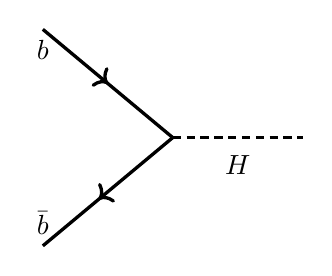
\begin{tikzpicture}[line width=0.9 pt, scale=1.1]
          \draw[particle] (-1.5,1.25) -- (0,0) node[pos=0.0,below]{$b$}; ;
          \draw[antiparticle] (-1.5,-1.25) -- (0,0) node[pos=0.0,above]{$\bar{b}$};
          \draw[scalar] (0,0) -- (1.5,0) node[midway,below=0.1cm] {$H$} ;
        \end{tikzpicture}
      \end{minipage}
      \begin{minipage}{0.32\linewidth}
        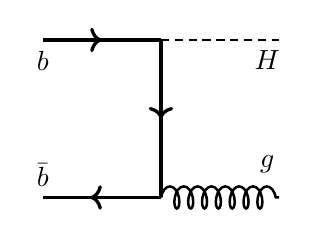
\begin{tikzpicture}[line width=0.9 pt, scale=1]
          \draw[particle] (-1.5,1.0) -- (0,1.) node[pos=0.,below] {$b$};
          \draw[antiparticle] (-1.5,-1.) -- (0,-1.) node[pos=0.0,above] {$\bar{b}$};
          \draw[particle] (0,1) -- (0.,-1);
          \draw[gluon] (0.,-1) -- (1.5,-1) node[pos=.9,above=5pt] {$g$};
          \draw[scalar] (0.,1) -- (1.5,1) node[pos=.9,below] {$H$};
        \end{tikzpicture}
      \end{minipage}
      \begin{minipage}{0.32\linewidth}
        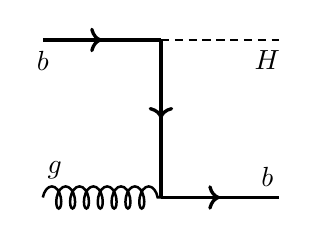
\begin{tikzpicture}[line width=0.9 pt, scale=1]
          \draw[particle] (-1.5,1.0) -- (0,1.) node[pos=0.,below] {$b$};
          \draw[gluon] (-1.5,-1.) -- (0,-1.) node[pos=0.1,above=3pt] {$g$};
          \draw[particle] (0,1) -- (0.,-1);
          \draw[particle] (0.,-1) -- (1.5,-1) node[pos=.9,above] {$b$};
          \draw[scalar] (0.,1) -- (1.5,1) node[pos=.9,below] {$H$};
        \end{tikzpicture}
      \end{minipage}
    }
    \caption{Feynman diagrams for the leading (left) and next-to-leading order real emission
      contributions to  Higgs production in bottom fusion which are present
      in the massive scheme when the $b$ quark PDF is independently
      parametrized, but absent otherwise.}
    \label{fig:massive-4fs}
  \end{figure}

  \subsection{Perturbative ordering}
\label{sec:pertord}


Because there is now a $b$ PDF also in the massive scheme, the
counting of perturbative orders in this scheme
changes substantially. Specifically, for Higgs production in bottom
fusion the diagrams of Fig.~\ref{fig:massive-4fs} are present only
when the $b$ PDF is independently parametrized. This means that while 
in the
massive scheme the process in the matched-$b$ approach of
refs.~\cite{Forte:2015hba,Forte:2016sja}  starts at $O(\alpha_s^2)$,
in a parametrized-$b$ approach it starts at 
$O(\alpha_s^0)$. As discussed in detail in
refs.~\cite{Forte:2010ta,Forte:2015hba,Forte:2016sja},
the FONLL method allows the  consistent combination of computations performed
at different perturbative orders either in the massive or massless
scheme: various combinations were defined and discussed  in
refs.~\cite{Forte:2015hba,Forte:2016sja} for Higgs production in
bottom fusion.

With the new counting of perturbative orders which is relevant for a
parametrized-$b$ framework it is convenient to define some new
combinations. We  consider in particular the combination of 
the massive scheme $O(\alpha_s)$ computation  with the standard
five-flavor scheme next-to-leading log (NLL) and
next-to-next-to-leading log  computations. We  call these
combinations respectively FONLL-AP (hence corresponding to NLO-NLL)
and FONLL-BP (corresponding to  NLO-NNLL).


\subsection{Parametrized-$b$ FONLL}
\label{sec:parbfonll}

The construction of the parametrized-$b$ FONLL for hadronic processes
closely follows the corresponding construction for electroproduction,
presented in refs.~\cite{Ball:2015tna,Ball:2015dpa}, to which we refer
for more details. In comparison to the matched-$b$ FONLL of
refs.~\cite{Forte:2015hba,Forte:2016sja} the massive scheme
contribution to Eq.~\eqref{eq:fonlldef} includes an extra contribution:
\begin{align}
  \label{eq:delta-i}
  \sigma_{\text{FONLL}_P} &= \sigma_{\text{FONLL}_M} +
  \delta\sigma_P\nonumber\\ 
  \quad \quad \delta\sigma_P &= \sigma^{\rm massive}_{P} - \sigma^{{\rm
      massive},0}_{P},
\end{align}
where $\sigma^{\rm massive}_{P}$ is the massive-scheme contribution to
the given process with initial-state heavy quarks and $\sigma^{{\rm
      massive},0}_{P}$ its massless limit (which subtract its double
counting with the massless-scheme contribution). This massive scheme
contribution has to be re-expressed in terms of massless-scheme PDFs,
as explained in detail in
refs.~\cite{Cacciari:1998it,Forte:2010ta,Ball:2015tna,Ball:2015dpa,Forte:2015hba,Forte:2016sja}.

For Higgs production in bottom fusion, up to NLO, this extra
contribution is given by
the real diagrams of Fig.~\ref{fig:massive-4fs}, supplemented
by the corresponding virtual correction and thus it
has the form
\begin{equation}
  \label{eq:xs4fs-i}
  \begin{split}
    \delta&\sigma_P^{\rm massive}\left(\frac{m_H^2}{m_b^2}\right) = 
    2\,\int_{\tau_0}^1 \frac{\dd{x}}{x}\,
    \int_{\frac{\tau_0}{x}}^1 \frac{\dd{y}}{y^2}\, \\
    &f^{(4)}_b(x)\,f^{(4)}_{\bar{b}}\left(\frac{\tau_0}{xy}\right)
    \biggl[\sigma_{b\bar{b}}^{(4),(0)}\left(y,\frac{m_H^2}{m_b^2}\right) +
      \alpha_s\,\sigma_{b\bar{b}}^{(4),(1)}\left(y,\frac{m_H^2}{m_b^2}\right)
    \biggr]\\
    &
    +
    4\,\alpha_s\,f^{(4)}_b(x)\,f^{(4)}_g\left(\frac{\tau_0}{xy}\right)\,
    \sigma_{bg}^{(4),(1)}\left(y,\frac{m_H^2}{m_b^2}\right)\,,
  \end{split}
\end{equation}
where the subscript $P$ denotes the fact that this contribution is
only present when the $b$ PDF is independently parametrized, and the
superscript $(4)$ is used to denote the massive factorization scheme,
as in refs.~\cite{Forte:2015hba,Forte:2016sja}. Note that even though,
with a parametrized $b$ there are five flavors also in
the massive scheme, only the four lightest ones contribute to
the running of $\alpha_s$ and perturbative evolution. The
massive cross-sections $\sigma_{ij}^{(4),(k)}$ were computed e.g. in
ref.~\cite{Krauss:2017wmx} based on corresponding QED results from
ref.~\cite{Dittmaier:1999mb} and are collected in
appendix~\ref{sec:app-coeff} after scheme change as we discuss below.

Note that in the matched-$b$ computation
of ref.~\cite{Forte:2015hba,Forte:2016sja} this
process  in the massive scheme starts at $O(\alpha_s^2)$, hence up to NLO (with our new
counting) the contribution given in Eq.~(\ref{eq:xs4fs-i}) is the only
one to $\sigma^{\rm massive}$ Eq.~(\ref{eq:fonlldef}): so in actual fact
in this case
\begin{equation}
   \sigma^{\rm massive,\,NLO}= \sigma^{\rm massive,\,NLO}_{P}.
\end{equation}

The expression of $\sigma^{\rm massive,\,NLO}$ suitable for use in the
FONLL formula Eq.~(\ref{eq:fonlldef}) is obtained, as mentioned, by
  re-expressing the massive scheme PDFs  and $\alpha_s$ in terms of massless-scheme
  ones. For simplicity we assume that this is done at a matching scale
  $\mu_b=m_b$.
  The matching condition for $\alpha_s$ is, as well known,
\begin{equation} \label{eq:amatch}
  \alpha_s^{(4)}(Q^2) = \alpha^{(5)}_s(Q^2)\left[1\,-\alpha_s\,\frac{T_R}{2\,\pi}\,\log\frac{Q^2}{m_b^2} + \order{\alpha_s^2}\right]
\end{equation}
while to $O(\alpha_s)$ the only nontrivial matching condition is
that for the $b$ PDF:
\begin{equation}
  \label{eq:b-pdf}
  \begin{split}
  f_b^{(4)}(x) = f^{(5)}_b(x,Q^2) - \alpha_s\int_x^1& \frac{\dd{z}}{z}
  \biggl[ K_{bb}^{(1)}\left(z,Q^2\right)f^{(5)}_b\left(\frac{x}{z},Q^2\right) \\
   &+ K_{bg}^{(1)}(z,Q^2)\,f_g^{(5)}\left(\frac{x}{z},Q^2\right)\biggr]+ \order{\alpha_s^2},
  \end{split}
\end{equation}
where again the superscripts $(4)$ and  $(5)$  denote  respectively the massive-
and massless-scheme expressions, and $K_{ij}$ are the matching
coefficients
\begin{equation}\label{eq:matching}
  f_i^{(5)}(Q^2) = \sum_j K_{ij}(Q^2) \otimes f^{(4)}_j(Q^2),
\end{equation}
where the sum runs over all partons (including the heavy quark),
and
\begin{equation}\label{eq:kexp}
  K_{ij}(Q^2)=\delta_{ij}\delta(1-z)+\sum_{n=1}\alpha^n_s(Q^2) K_{ij}^{(n)}(Q^2).
\end{equation}
Note
that, of course, since there is a heavy quark PDF also in the massive
scheme, $K_{ij}$ is a square matrix, so that, to $O(\alpha_s)$,
$  K^{-1}_{ij}(Q^2)=\delta_{ij}-\alpha_s(Q^2) K_{ij}^{(1)}(Q^2)$.
The matching function 
 $K^{(1)}_{bb}$ was calculated in ref.~\cite{Buza:1996wv}. Its explicit
expression is given for ease of reference in appendix~\ref{sec:app-splitting} together with
that of the splitting functions
$P_{ij}$. 

Substituting Eqs.~(\ref{eq:amatch}-\ref{eq:b-pdf}) in
Eq.~(\ref{eq:xs4fs-i}) we get the desired expression for the
massive-scheme cross section:
\begin{equation}
  \label{massive:1}
  \begin{split}
  \sigma_P^{\rm
    massive}\left(\frac{m_H^2}{m_b^2}\right)&=
  \int_{\tau_H}^{1} \frac{dx}{x}\int_{\frac{\tau_H}{x}}^{1}
  \frac{dy}{y^2} \\
  &\sum_{ij=b,g}f_{i}^{(5)}(x,Q^2)f_j^{(5)}
  \left(\frac{\tau_H}{x y},Q^2\right)
  B_{ij}\left(y,\alpha_s^{(5)}(Q^2),
    \frac{Q^2}{m_b^2}\right),
  \end{split}
\end{equation}
where to $O(\alpha_s)$ the non-vanishing coefficients are 
\begin{align}
  \label{eq:change-of-scheme}
  B_{b\bar{b}}^{(0)}\left(y,\frac{m_H^2}{m_b^2}\right)  
    & = \sigma_{b\bar{b}}^{(4),(0)}\left(y,\frac{m_H^2}{m_b^2}\right) \\
  B_{b\bar{b}}^{(1)}\left(y,\frac{m_H^2}{m_b^2}\right)
    & = \sigma_{b\bar{b}}^{(4),(1)}\left(y,\frac{m_H^2}{m_b^2}\right) \nonumber\\ 
    & - 2\,\sigma_0
      \int_{y}^{1}{\rm d} z \,z\,\delta(z-y)\,
      K_{bb}^{(1)}\left(z,\ln\frac{m_H^2}{m_b^2}\right)\\
  B_{bg}^{(1)}\left(y,\frac{m_H^2}{m_b^2}\right)
    & = \sigma_{bg}^{(4),(1)}\left(y,\frac{m_H^2}{m_b^2}\right) \nonumber \\
    &  -\sigma_0
      \int_{y}^{1}{\rm d} z \,z\,\delta(z-y)\,
      K_{bg}^{(1)}\left(z,\ln\frac{m_H^2}{m_b^2}\right)\,,
\end{align}
whose explicit expressions are collected, as mentioned, in appendix~\ref{sec:app-coeff}.

In order to construct the FONLL expression Eq.~(\ref{eq:fonlldef}), the
massive scheme contribution must be combined with the difference term
$\sigma ^{\rm d}$ Eq.~(\ref{eq:fonlldiff}). However, it is easy to
check that, just like in the case of
electroproduction\cite{Ball:2015tna,Ball:2015dpa},
this term, which is subleading when using matched $b$, vanishes
identically with parametrized $b$. This is due to the
fact that the massless limit of the massive-scheme calculation only
differs from the massless-scheme calculation because of the resummation
of mass logarithms $\ln\frac{Q^2}{m_b^2}$ beyond the accuracy of the
massive-scheme result (so at $O(\alpha_s^2)$ and beyond, in our
case). However, when re-expressing the massive-scheme calculation in
terms of massless-scheme PDFs the evolution of the $b$-PDF is only
removed up to the same accuracy as that of the massive scheme
calculation. This is seen explicitly in Eq.~(\ref{eq:b-pdf}), in which
mass logarithms  $\ln\frac{Q^2}{m_b^2}$ are only removed up to
$O(\alpha_s)$. Therefore, the higher order logarithms remain unsubtracted in
the expression of $f_b^{(5)} (x,Q^2)$ and thus cancel exactly between
$\sigma^{\rm massless}$ and $\sigma^{\rm massive,\,0}$.

The FONLL
result thus reduces to the expression Eq.~(\ref{massive:1}):
\begin{equation}\label{eq:canc}
\sigma^{\text{FONLL-AP}}=\sigma_P^{\rm
  massive}\left(\frac{m_H^2}{m_b^2}\right).
\end{equation}
We can thus write the FONLL result in the form
\begin{equation}\label{eq:genfonll}
\sigma^{\text{FONLL-AP}}= \sum_{i,j}\sum_{l,m} \sigma^{\rm massive}_{ij}\left(\frac{m_h^2}{m^2_b}\right)\otimes
 K^{-1}_{il}\otimes f_{l}^{\left(5\right)}\left(Q^2\right)K^{-1}_{jm}\otimes f_{m}^{\left(5\right)}\left(Q^2\right),
\end{equation}
where $ K^{-1}_{il}$ is the inverse of the matching matrix defined in
Eq.~(\ref{eq:amatch}), perturbatively defined order by order according
to Eq.~(\ref{eq:kexp}). This is
of course  well defined with a parametrized $b$ because
$K_{ij}$ is  a square matrix. As discussed in detail in
refs.~\cite{Ball:2015tna,Ball:2015dpa} the effect of the inverse
matching matrices in Eq.~(\ref{eq:genfonll}) is to remove collinear
logarithms related to the evolution of the $b$ PDF from the massless scheme
PDFs $f_{i}^{\left(5\right)}$, since these are already included in the
massive-scheme matrix cross-section  $\sigma^{\rm massive}_{ij}$,
where they would appear as mass logarithms $\ln\frac{Q^2}{m_b^2}$
in the large $Q^2$ limit (in actual facts here $Q^2=m_H^2$). As a
consequence, the result Eq.~(\ref{eq:genfonll}) is completely
independent of the matching scale $m_b$ (i.e. the scale at which the
$b$ PDF is parametrized), as it must be, given that once
the $b$ PDF is parametrized there is no matching scale left.
We will check this cancellation explicitly (see 
Fig.~\ref{fig:mub-var} below).

Equation~(\ref{eq:genfonll}) shows that FONLL effectively acts
as a massive five-flavor scheme, in which standard five-flavor PDFs
are combined with the massive-scheme cross-section, with massive
quarks included in the initial state: it is in fact akin to 
five-flavor scheme of ref.~\cite{Krauss:2017wmx}, though in this
reference mass effects are also included in parton showering, which we
do not consider here. In FONLL corrections are consistently
included to the order at which the massive-scheme cross-section is
computed, with collinear and mass logarithms resummed to the logarithmic
order to which PDFs are used. The structure of the result
Eq.~(\ref{eq:genfonll}) is universal, and so are the PDFs which appear
in it. Therefore, to the extent that the  PDF is correctly fitted,
mass corrections (i.e. all terms suppressed by powers of $m_b/Q$) are
then fully included  up to the order of the massive-scheme
calculation:   $O(\alpha_s)$ for FONLL-AP and FONLL-BP. Of course
these latter corrections are not universal and will have to be computed
separately for each process.

As mentioned, the FONLL framework
allows for the combination of massive- and massless-scheme
computations performed at arbitrary, independent accuracy. We discuss
specifically the two cases defined in Sect.~\ref{sec:pertord}, FONLL-AP and
FONLL-BP. In FONLL-AP, the massive-scheme partonic cross sections 
 $\sigma_{ij}^{\rm massive}$ are computed up to NLO
(i.e. $O(\alpha_s)$), while the PDFs are evolved using 
NLO (more properly, NLL) evolution equations. Hence, in this case
Eq.~(\ref{eq:genfonll}), with  $\sigma_{ij}^{\rm massive}$ computed up
to $O(\alpha_s)$ (i.e. including the diagrams of
Fig.~\ref{fig:massive-4fs}), and NLO PDFs.  


In FONLL-BP, the
massive-scheme computation is still performed up to NLO, but now the
massless-scheme computation is performed up to NNLO. This has two
consequences. The first is that NNLO PDFs are now used. The other is
that hard cross-sections are now computed up to NNLO i.e. up to
$O(\alpha^2_s)$. Because massive terms are included only up to
$O(\alpha_s)$, Eq.~(\ref{eq:genfonll}) must now be supplemented by a
purely massless $O(\alpha^2_s)$ contribution:
\begin{equation}\label{eq:fonll-bp}
\sigma^{\text{FONLL-BP}}=\sigma^{\text{FONLL-AP}}+\sum_{l,m}
\sigma^{(5),(2)}_{lm}\otimes
f_{l}^{\left(5\right)}\left(Q^2\right)f_{m}^{\left(5\right)}\left(Q^2\right), 
\end{equation}
where $\sigma^{\text{FONLL-AP}}$ is given by
Eq.~(\ref{eq:genfonll}). Note that because the matching functions
$K_{ij}^{-1}$ are 
used to re-express the massive-flavor scheme cross-section in the
massless scheme, they are accordingly  computed to the same accuracy as
the massive-scheme partonic cross-section itself: so here
to $O(\alpha_s)$. The difference term $\sigma^{\rm d}$
Eq.~(\ref{eq:fonlldiff}) always vanishes identically. It is clear
that the computation is considerably streamlined in comparison to the
standard FONLL framework of refs.~\cite{Forte:2015hba,Forte:2016sja}.

\section{Higgs production in $b$ fusion}
\label{sec:results}


We now present explicit results for Higgs production in $b$-quark fusion
within the FONLL-AP and FONLL-BP scheme, and compare them to previous
results of refs.~\cite{Forte:2015hba,Forte:2016sja}.
Results presented in this section are obtained using
the following set-up.
For the calculation of the 5F scheme coefficient functions,
we use the interface to the {\verb bbh@nnlo }
code~\cite{Harlander:2002wh}
as implemented in the public {\tt bbhfonll} code~\cite{code}.
The subtraction terms needed for the FONLL-B calculation of
refs.~\cite{Forte:2015hba,Forte:2016sja} 
is obtained using  {\tt bbhfonll}. The standard contributions
to the 4F scheme are computed
using the MG5\_aMC@NLO package~\cite{Alwall:2014hca,Wiesemann:2014ioa},
while we have implemented the new terms $\delta\sigma_P^{\rm massive}$
Eq.~(\ref{eq:xs4fs-i})
and their
massless limit in a new version of  {\tt bbhfonll}, following
the expressions reported in appendix~\ref{sec:app-coeff}.
Both codes use the LHAPDF~\cite{Buckley:2014ana} package.

We use the  NNPDF3.1 NNLO set of parton distributions with
$\alpha_s(M_z)=0.118$~\cite{Ball:2017nwa}. For a first default
comparison we just use the default NNPDF3.1 set, including the $b$
PDF. From the point of view of a computational framework in which the
$b$ PDF is fitted,
this can be thought of as the $b$ PDF that one would get if initial
PDFs were parametrized at $Q_0=m_b$, and the fitted $b$ PDF were to
turn out to be exactly equal to that given by the matching condition
at this scale. Furthermore, in order
to get a feeling for effects related to the size of
the $b$-PDF we then consider, for the sake of argument, a $b$ PDF
equal to that which would be obtained by using the matching condition
at $\mu_b = 2/3 m_b$ or $\mu_b = 1/2 m_b$, and then evolving up to
$Q=m_b$ where the initial PDF is given.

\begin{figure}[htbp]
  \centering
  \includegraphics[width=0.6\textwidth]{mub_var.pdf}
  \caption{Cancellation of the dependence on the matching scale in the
  FONLL-AP and FONLL-BP schemes.}
  \label{fig:mub-var}
\end{figure}
First, as a consistency check, in Fig.~\ref{fig:mub-var} we verify that
indeed the dependence on $\mu_b$ cancels when constructing the FONLL
result with parametrized $b$ according to Eq.~(\ref{eq:delta-i}). In
this figure the massive-scheme result has been constructed using a
fixed  $b$ PDF (that which corresponds to the standard matching
condition at $\mu_b=m_b$) and then re-expressing results in terms of
the massive scheme PDFs  and $\alpha_s$ in terms of massless-scheme
ones. This is done using Eq.~(\ref{eq:matching}), which contains the
matching coefficients $K_{ij}$ which depend on the matching scale
$\mu_b$, and thus the massive-scheme result becomes
$\mu_b$-dependent.
However, this dependence cancels exactly in the final
FONLL result.

\begin{figure}[htbp]
  \centering
  \includegraphics[width=0.49\linewidth]{mur_var_nnpdf_.pdf}
  \includegraphics[width=0.49\linewidth]{muf_var_nnpdf_.pdf}
  \caption{Renormalization (left) and factorization (right) scale
    variation of the cross-section for Higgs production in bottom
    fusion. The pure five-flavor scheme computation is compared to the
  FONLL-AP and FONLL-BP results presented here and to the FONLL-B
  result of ref.~\cite{Forte:2015hba}. For the pure five flavor
  NNLO and the  FONLL-BP three curves are shown, corresponding to 
  three choices of initial $b$ PDF (see text).
  }
  \label{fig:scale-var}
\end{figure}


In Fig.~\ref{fig:scale-var} we show the factorization and
renormalization scale dependence of the cross-section computed in
various schemes, with the other scale kept fixed at the
preferred~\cite{Forte:2015hba,Forte:2016sja} value
$\mu=\frac{m_H+2m_b}{4}$.
Specifically, we compare results obtained using the FONLL-AP and
FONLL-BP schemes discussed above, the pure five-flavor scheme , and
the FONLL-B result of ref.~\cite{Forte:2016sja}, all using the same
PDFs (including the $b$ PDF) as discussed above. For the pure
five-flavor scheme and for FONLL-BP we also show
the three curves corresponding to the three different choices for the
$b$ PDF discussed above, with a corresponding band:
the central, thick, solid line represents the default $\mu_b=m_b$
choice, while the edges of the band are drawn with dot-dash curves
with decreasing thickness, with the thicker of the two corresponding
to $\mu_b=2\frac{m_b}{3}$, and the other two $\mu_b=\frac{m_b}{2}$.

Note that the
FONLL-BP computation Eq.~(\ref{eq:fonll-bp}) and the FONLL-B
result~\cite{Forte:2016sja} are directly comparable: indeed, they both
include the five-flavor scheme computation up to NNLO, and combine it
with the first
two orders of the massive-scheme computation. The difference is that
in FONLL-B in the massive-scheme computation refers to the process
$gg\to b\bar b H$, while in FONLL-BP it refers to  $b\bar b \to H$. If
the $b$ PDF is the same as given by perturbative matching, the
difference is then only that, in the latter case, only mass effects
related to the $b\bar b$ which fuses into the Higgs are included,
while in the former, also those related to the further unobserved
$b\bar b$ pair are present. In a realistic situation, in which FONLL-BP is used
while parametrizing and fitting the $b$ PDF these mass effects should
be reabsorbed in the fitted $b$ PDF. In our comparisons, they 
appear as a certain enhancement of FONLL-BP in comparison to FONLL-B
due to the opening of phase space. 


Otherwise, the qualitative features of the comparison between FONLL
and the pure five-flavor scheme remain essentially the same as discussed
in ref.~\cite{Forte:2016sja}: FONLL is quite close to the
five-flavor scheme, with mass effects a non-negligible, but small,
positive correction. Indeed, the difference between
FONLL-AP and FONLL-BP, i.e., the impact of NNLO corrections in the
five-flavor scheme, is much more significant than that of mass corrections.
The impact of varying the $b$ PDF by
an amount which is comparable to a reasonable variation of the
matching scale is clearly comparable to that of the mass
corrections. This provides evidence for the fact that fitting the $b$
PDF is likely to have a significant impact on precision phenomenology.


Note that results for the FONLL-B
scheme differ at the percent level from those of 
ref.~\cite{Forte:2016sja} because there a different PDF set and $m_b$
value were used,
for the sake of benchmarking with
ref.~\cite{Bonvini:2015pxa,Bonvini:2016fgf}. This further highlights
the fact that the size of effects due to the $b$ PDF is comparable to
that of mass corrections.

In summary, we have shown how the FONLL matching of massive- and
massless-scheme treatment of computations involving heavy quarks can
be generalized to the case in which the heavy quark PDF is freely
parametrized for hadronic processes. We have show that this
effectively provides us with a massive heavy quark scheme, in which
the heavy quark is endowed with a standard PDF satisfying QCD
evolution equations, yet it is treated as massive in hard matrix
elements. A first application to Higgs production in bottom fusion
shows that effects related to the $b$ PDF are quite likely to be
comparable to mass corrections: both are small, but non-negligible
corrections to a purely massless NNLO calculation in which the $b$ PDF
is obtained from perturbative matching conditions. Determining the $b$
PDF from data is thus likely to be necessary for a description of
$b$-induced hadron collider processes at percent or sub-percent accuracy.

As a direction for further study, it should be noticed that extending
our results to NNLO --- thereby allowing the construction of a
FONLL-CP result, in the terminology of Sect.~\ref{sec:pertord}
(NNLO+NNLL) --- is beyond current knowledge. Indeed, starting at NNLO
the cancellation between real and virtual
corrections is no longer trivial, and is spoiled by
massive quarks in the initial
state~\cite{Doria:1980ak,Catani:1985xt}. 
This problem has been recently revised in ref.~\cite{Caola:2020xup}.
Hence, such an extension to NNLO
would require conceptual advances in the understanding of QCD
factorization in the presence of massive quarks, which are left for
future studies.


\chapter{PDFs from lattice data}
\label{ch:lattice}

\chapter{PDFs from quasi-PDFs matrix elements}
Data for equal-time correlators coming from first lattice QCD simulations
have started appearing and have gotten into already a relatively advanced stage over the last few years
\cite{Lin:2014zya,Alexandrou:2015rja,Chen:2016utp,Alexandrou:2016jqi,Zhang:2017bzy,Alexandrou:2017huk,Lin:2017ani,Chen:2017gck,Alexandrou:2018pbm,Chen:2018xof,Chen:2018fwa,Alexandrou:2018eet,Liu:2018uuj,Lin:2018qky,Fan:2018dxu,Liu:2018hxv,Alexandrou:2019lfo,Izubuchi:2019lyk}.
This gives an idea of what PDFs from the lattice might look like, not only for
nonsinglet quark PDFs of the nucleon, but also for the pion PDF and distribution
amplitude, as well as for the gluon PDF of the nucleon. Given the general
interest shown by the community, a quick improvement in the technologies
involved in such lattice simulations is to be expected in the next few years. A
great quantity of increasingly precise lattice data is then likely to be
available in the near future, requiring detailed studies about the possible
impact they might have on the overall precision of PDFs determination.

Despite the increasing number of numerical results becoming available, an
optimal strategy for reconstructing the PDFs from these data has not been
entirely addressed yet. The approach which has been initially used within the lattice community
(and that is still employed in many analyses)
consists in approximating the quasi- or pseudo-PDFs by mean of a discrete Fourier transform,
starting from the limited number of points for the corresponding equal-time correlator available from numerical simulations. 
The continuous function resulting from this procedure
is subsequently convoluted with the perturbative matching coefficients relating euclidean and light-cone distributions,
in order to obtain the final PDF.
The numerical error introduced by this procedure is rather large and difficult to control,
so that this procedure generally provides unstable and inaccurate results.
This problem was first addressed within the lattice community in Ref.~\cite{Karpie2019}
where a series of possible approaches to tackle the problem of incomplete and discretized Fourier
transform has been presented.

In this Chapter, we exploit the momentum space factorization of quasi-PDFs in PDFs and perturbatively
computable coefficients to extract nonsinglet distributions from the data of
Refs.~\cite{Alexandrou:2018pbm,Alexandrou:2019lfo}, using the {\tt NNPDF} framework described
in Chapter~\ref{ch:nnpdf_methodology} and treating the lattice data on the same footing as experimental ones.

%The discussion is focused on the
%quasi-PDFs case, but it can be extended to include data coming from different
%lattice approaches, like for example pseudo-PDFs
%\cite{Radyushkin:2017cyf,Orginos:2017kos,Karpie:2018zaz}, fictitious heavy/light
%quark~\cite{Detmold:2005gg,Braun:2007wv} or current-current correlators
%\cite{Ma:2014jla,Ma:2017pxb,Sufian:2019bol}, paving the way to a first global
%lattice QCD analysis~\cite{Ma:2017pxb}.

\section{quasi-PDFs in QCD}
%
Denoting by $\Gamma$ a generic Dirac structure and by the suffix $A$ the specific nonsinglet distribution
we want to consider, we can introduce the {\em Ioffe time distributions} \cite{Radyushkin:2017cyf,Braun:1994jq}, 
defined as the matrix element between nucleon states with momentum $P$
\begin{align}
	\label{eq:Ioffe}
	M^\bare_{\Gamma,A}\left(z,P\right) &= \langle P |\mathcal{M}^\bare_{\Gamma,A}\left(z\right) |P\rangle \, ,
\end{align}
with
\begin{align}
	\label{eq:bilocal}
	\mathcal{M}^\bare_{\Gamma,A}\left(z\right)= \bar{\psi}^\bare\lp z\rp \lambda_A \Gamma \,   
	U\lp z,0\rp \psi^\bare\lp 0\rp.
\end{align}
Eqs.~\eqref{eq:Ioffe}, \eqref{eq:bilocal} represent the QCD generalization of the scalar quantity defined 
in Eq.~\eqref{eq::ME}.
The vector bilocal operator obtained for $\Gamma=\gamma^\mu$ can be decomposed
in terms of two form factors depending on Lorentz invariants:
\[
    \label{eq:IoffeDecomposition}
    M^\bare_{\gamma^\mu,A}\left(z, P\right)
    = 2 P^\mu\,\text{h}^{(0)}_{\gamma^\mu,A}\lp z\cdot P,z^2 \rp
    + z^\mu\, \tilde{\text{h}}^{(0)}_{\gamma^{\mu},A}\lp z\cdot P,z^2 \rp \, . 
\]
The light-cone PDF in Eq.~\eqref{eq:fADef} is obtained by taking the Fourier
transform with respect to $z^-$ of a Ioffe time distribution with $\Gamma =
\gamma^+$, $z=\left(0,z^-,0_{\perp}\right)$ and $P=(P^+,0,0_{\perp})$, given
by
\begin{align}
	\label{eq:Ioffelightcone}
    M^\bare_{\gamma^+,A}\left(z,P\right) =  
    \langle \text{P}|\bar{\psi}^\bare\lp z^-\rp \lambda_A \gamma^+ \,   
	U\lp z^-,0\rp \psi^\bare\lp 0\rp  |\text{P}\rangle
	= 2 P^+\,\text{h}^{(0)}_{\gamma^+,A}\lp z^- P^+,0 \rp\, .
\end{align} 
Choosing instead a pure spatial direction $z=\left(0,0,0,z\right)$, and taking
the Fourier transform with respect to $z$, we obtain the definition of the
quasi-PDF  
\begin{align}
	\label{eq::bareqpdf}                                                 
	\tilde{f}_A^{(0)}\lp x, P_z\rp = 
	\int_{-\infty}^{\infty}\frac{dz}{4\pi}\,e^{i x \text{P}_z z}\,M^\bare_{\Gamma,A}\left(z,P\right)\, .
\end{align}
Choosing for example $\Gamma = \gamma^0$ we get
\begin{align}
	\label{eq::bareqpdf}                                                 
	\tilde{f}_A^{(0)}\lp x, P_z\rp = 
	2 P_0 \, \int_{-\infty}^{\infty}\frac{dz}{4\pi}\,e^{i x \text{P}_z z}\,\text{h}^{(0)}_{\Gamma,A}\lp z P_z,z^2 \rp, 
\end{align}
which will be the case considered in this work. As in the case of standard PDFs
(which from now on we will call {\em light-cone}\ PDFs), the matrix elements
defining the quasi-PDFs contain UV divergences, and need to be renormalized. The
main features of the perturbative renormalization of a bilocal operator, 
as the one appearing in
Eq.~\eqref{eq::bareqpdf}, have been described in Chapter~\ref{ch:scalar_model}
in the context of the scalar theory.
Despite the details of the full QCD computation are of course more complicate,
see Ref.~\cite{Ishikawa:2017faj}, as mentioned before 
its main features and results are well described by the simple scalar case.
As we found out looking at the scalar QFT,
the position space operator appearing in Eq.~\eqref{eq::bareqpdf} can be multiplicatively
renormalized, according to
\begin{align}
    \text{h}_{\Gamma,A}\lp z P_z,z^2,\mu \rp = Z_{A}(z)\,
    e^{\delta m |z|} \text{h}^\bare_{\Gamma,A}\lp z P_z,z^2 \rp\,.
\end{align}
The only difference with respect to the scalar case is given by
the exponential factor $e^{\delta m |z|}$, which reabsorbs the power divergence
from the Wilson line which appears in the QCD case. The position-dependent factor $Z_{A}(z)$ takes care of
the remaining UV logarithmic divergences.  
%
Importantly, we recall that the quasi-PDFs retain a dynamical dependence on the hadron momentum
$P$, unlike PDFs, which are defined to be invariant under Lorentz boosts. Also,
their support is defined to be the full real axis.

The interest in quasi-PDFs comes from the potential to relate them to light-cone
PDFs, as detailed in Sec.~\ref{sec::momentumspace};
factorization allows us to rewrite the quasi-PDFs as a convolution of the
light-cone PDFs with a coefficient function that can be computed in perturbation
theory, up to corrections that are suppressed by inverse powers of $P_z$.
It follows that they can be written as
\begin{align}
	\label{eq::pdftoqpdf}                                                                             
	\tilde{f}_A\lp x , {\mu}^2 \rp =                                                               
	\int_{-1}^{1} \frac{dy}{|y|}\, C_A\lp\frac{x}{y},\frac{\mu}{|y|P_z},\frac{\mu}{\mu'} \rp  f_A\lp y, {\mu'}^2\rp 
	+ \mathcal{O}\lp \frac{M^2}{P_z^2},\frac{\Lambda^2_{\text{QCD}}}{P_z^2} \rp\, ,                   
\end{align}
where the terms $\mathcal{O}\lp
\frac{M^2}{P_z^2},\frac{\Lambda^2_{\text{QCD}}}{P_z^2} \rp $ include
the power corrections suppressed by the hadron momentum. The functions $C_A$,
usually called matching coefficients, depend on the choice of the
renormalization scheme, and on the kind of quasi-PDF under consideration. The
first matching expressions, for all Dirac structures, were derived in
Ref.~\cite{Xiong:2013bka}, using a simple transverse momentum cutoff scheme. In
later works, matching coefficients were derived that relate the quasi-PDFs in
different renormalization schemes to light-cone PDFs in the $\MSb$ scheme. The
matching from $\MSb$ quasi-PDFs was first considered in
Ref.~\cite{Wang:2017qyg}, both for non-singlet and singlet quark PDFs, as well
as for gluons. Even though one can choose operators for the latter that do not
mix with singlet quark quasi-PDFs under
renormalization~\cite{Zhang:2018diq,Li:2018tpe}, mixing under matching is
inevitable. 
No mixing of the flavour nonsinglet sector with flavour singlet or
gluon sectors occurs, as stated in Eq.~\eqref{eq::pdftoqpdf}. Ref.~\cite{Wang:2017qyg} did not, however, address the
known issue of self-energy corrections, exhibiting a logarithmic UV divergence.
This was resolved in Ref.~\cite{Izubuchi:2018srq} by adding terms outside of the
plus prescription in the matching coefficient. As noticed in
Ref.~\cite{Alexandrou:2018pbm}, such prescription for renormalizing this
divergence violates vector current conservation, \ie\ the integral of the
matched PDF is different from the integral of the input quasi-PDF, and not
necessarily equal to 1 over the whole integration range. As a remedy, a modified
matching expression, which is given explicitly in Eq.~\eqref{eq::matching} of
App.~\ref{app:coefficients}, was proposed in Ref.~\cite{Alexandrou:2018pbm}. It
consists in resorting to pure plus functions when subtracting the logarithmic
divergence in self-energy corrections. However, this is an additional
subtraction with respect to the minimal subtraction of the $\MSb$ scheme and
thus, defines a modified $\MSb$ scheme, the so-called $\MMSb$ scheme. As such,
it requires the quasi-PDF to be expressed in this modified scheme. The
expression for the conversion of $\MSb$-renormalized matrix elements to the
$\MMSb$ scheme was worked out in Ref.~\cite{Alexandrou:2019lfo} and we refer to
it for the details of the procedure. Nevertheless, this modification is
numerically very small, as also shown in Ref.~\cite{Alexandrou:2019lfo}. An
alternative modification of the $\MSb$ scheme that guarantees vector current
conservation was derived in an updated version of Ref.~\cite{Izubuchi:2018srq}.
This defines the so-called ``ratio'' scheme. In this scheme, only pure plus
functions are used, like in the $\MMSb$ scheme, but the modification is done
also for the ``physical'' region of $0<z<1$ (in the notation of
Eq.~\eqref{eq::matching}). Thus, the expected numerical effect of this
modification is larger, as shown explicitly in Ref.~\cite{Alexandrou:2019lfo}.
For this reason, we choose to use the $\MMSb$ procedure, with details of the
lattice computation of the bare matrix elements and the renormalization in the
$\MMSb$ scheme outlined in the next section. Yet another possibility of
performing the matching consists in directly relating the quasi-PDFs in the
intermediate RI-type scheme to $\MSb$ light-cone PDFs. This was proposed in
Ref.~\cite{Stewart:2017tvs} for the unpolarized case. Obviously, such
procedure is equivalent to the one adopted here, with possibly different
systematic effects. All of the discussed papers considered the matching to only
first order in perturbation theory, but NNLO results for the matching coefficients have recently become available
in both position and momentum space \cite{Li:2020xml, Chen:2020ody, Braun:2020ymy, Chen:2020arf, Chen:2020iqi}.


\chapter{PDFs from pseudo-Ioffe Time Distribution}
\label{ch:ppdf_NNPDF}
In the previous Chapter, 
starting from the momentum space factorization formula connecting quasi-PDFs to collinear PDFs,
upon numerical implementation of the Fourier transform an expression relating
parton distributions directly to position space quasi-PDFs matrix elements
was obtained. Such factorized expression has been subsequently used in the NNPDF framework in order to 
extract two nonsinglet distributions from data for quasi-PDFs matrix elements 
produced in Refs.~\cite{Alexandrou:2018pbm, Alexandrou:2019lfo}.
A similar analysis was very recently performed by the JAM collaboration in Ref.~\cite{Bringewatt:2020ixn} 
for the spin-averaged and spin-dependent PDFs employing quasi-PDF lattice data.  
In this Chapter, base on Ref.~\cite{DelDebbio:2020rgv} we extend such analysis to the case of the pseudo-PDFs approach,
which relies on the position space formulation of the same factorization theorem. 
In particular, we will consider data for reduced pseudo-ITD, introduced in Sec.~\ref{sec:pseudo_PDFsfact}
in the context of the scalar field theory.

%
As we saw in Sec.~\ref{sec:qPDFs_th} the UV divergences of the Ioffe-time pseudodistribution (pseudo-ITD)
are multiplicatively renormalizable~\cite{Ji:2017oey,Ishikawa:2017faj}. 
The relevant renormalization factor $Z(z_3^2)\,e^{\delta m |z|/a}$ does not depend on $\nu$ and, 
for small $z_3^2$,   is known at one loop. 
Its explicit form is inessential if one introduces the so-called reduced 
Ioffe-time pseudo-distributions first defined in Ref.~\cite{Radyushkin:2017cyf}
as 
\begin{align}
	\label{eq:reducedIoffe}
	\mathfrak{M}\left(\nu, z_3^2\right) = \frac{\mathcal{M}\lp \nu,-z_3^2, \mu^2 \rp}{\mathcal{M}\lp 0,-z_3^2, \mu^2 \rp}. 
\end{align}
The $Z$-factors of the numerator and denominator are the same and cancel in the ratio leaving the reduced distribution
on the left-hand side without any residual dependence on 
unphysical scales. 


Working in the small-$z_3^2$ limit, the pseudo-ITD can be matched at one-loop level to the corresponding ITD
through a finite perturbative kernel, expressing the pseudo-ITD in terms of the collinear PDFs through a factorization formula
based on the operator product expansion (OPE).  
The computation of the relevant QCD diagrams has been performed in a number of independent papers.
The original QCD computation is reported, for example, 
in Refs.~\cite{Radyushkin:2017lvu, Radyushkin:2016hsy, Izubuchi:2018srq, Ji:2017rah}.
A simple discussion of the basic features of  the derivation of the factorization formula in non-gauge 
theories has been presented in Chapter~\ref{ch:scalar_model}, following Ref.~\cite{DelDebbio:2020cbz}.
The QCD result reads
\begin{align}
	\label{eq:factIoffe}
	\mathfrak{M}\left(\nu, z_3^2\right) = \int_{-1}^{1} dx\,C\left(x\nu,\mu^2 z_3^2\right)f\left(x,\mu^2\right) + \mathcal{O}\left(z_3^2\Lambda^2\right)\,, 
\end{align}
with
\begin{align}
	\label{eq:WilsonCoeffIoffe}
	C\left(\xi,\mu^2 z_3^2\right) 
	= e^{i\xi} \nonumber -\frac{\alpha_s}{2\pi}& C_F \int_0^1 dw \, \biggl[\frac{1+w^2}{1-w} \log\left(z_3^2\mu^2\frac{e^{2\gamma_E + 1}}{4}\right) \nonumber \\
	&+4\frac{\log\left(1-w\right)}{1-w} -2\left(1-w\right)\biggr]_+ e^{i \xi w} + \mathcal{O}\left(\alpha_s^2\right).
\end{align}
Eqs.~\eqref{eq:factIoffe}, ~\eqref{eq:WilsonCoeffIoffe} allow to relate collinear PDFs to quantities
which are computable in lattice QCD simulations, through a factorized expression similar to those
relating collinear PDFs to physical cross sections. Just as described in the previous Chapter, 
this formula can be used in a fitting framework to extract PDFs from lattice data.

%
%In this Chapter we perform an analogous exercise considering this time the reduced pseudo-ITD approach,
%implementing within the {\tt NNPDF} environment the lattice data presented in Ref.~\cite{Joo:2019jct,Joo:2020spy},
%and using the position space factorization formula of Eqs.~\eqref{eq:factIoffe}, \eqref{eq:WilsonCoeffIoffe}.
This, besides being a complementary exercise to the one performed in Ref.~\cite{Cichy2019}, has also some
practical advantages. First, when working in the pseudo-ITD approach, the factorization is realized in the limit of small-$z^2$.
Unlike in the quasi-PDFs approach, where the factorization is realized for high values of $P$,
here we are allowed to keep in the analysis data coming from a wide range of momentum values, 
without having to remove those with lower $P$.
This advantage is particularly important, because in lattice QCD, the low momentum data are significantly more precise for a fixed computational cost.
Second, we can directly use the position space factorization formula of Eq.~\eqref{eq:factIoffe}, relying on the analytical
expression for the perturbative coefficient of Eq.~\eqref{eq:WilsonCoeffIoffe} and without having
to perform the numerical Fourier transform described in App.~\ref{app:coefficients}.

\iffalse
In this article we extend the general strategy that has been developed within the {\tt NNPDF} framework and which allows us to systematically extract parton distributions from the available lattice data. In the implementation of this idea once the lattice data have reached some level of maturity in terms of precision and systematic effects, one could combine data from all pertinent lattice formalisms such as quasi-distributions ~\cite{Lin:2014zya,Chen:2016utp,Alexandrou:2015rja,Alexandrou:2016jqi, Monahan:2016bvm, Zhang:2017bzy, Alexandrou:2017huk, Green:2017xeu,Alexandrou:2018pbm,Chen:2018xof,Alexandrou:2018eet,Lin:2018qky,Fan:2018dxu,Liu:2018hxv,Alexandrou:2019lfo,Izubuchi:2019lyk,Green:2020xco,Chai:2020nxw,Lin:2020ssv,Alexandrou:2020zbe}
and pseudo-distributions ~\cite{Orginos:2017kos,Karpie:2018zaz,Joo:2019jct,Joo:2019bzr,Joo:2020spy,Bhat:2020ktg,Fan:2020cpa,Gao:2020ito}.
One can also include results from the so-called ``Good Lattice Cross-Sections'' (LCS) approach,
which is described in~\cite{Ma:2017pxb} and represents a general framework, where one computes matrix elements that can be factorized into PDFs at short distances. 
Papers~\cite{Bali:2017gfr,Bali:2018spj,Sufian:2019bol,Bali:2019ecy, Sufian:2020vzb} describe implementations of the latter formalism.
Clearly a global analysis only makes sense after having scrutinised each set of data individually,
and having understood the systematics that affect them.
\fi
The structure of the Chapter is as  follows.  In Sec.~\ref{sec:data} we define the lattice observable considered in the fit,
describe the corresponding data and  briefly recall the main features of the NLO terms entering the factorization formulas.
In Sec.~\ref{sec:fit} we present the first set of results:
we consider the  fits where only the statistical uncertainties of the lattice data are taken into account.
Analyzing data from different lattice ensembles we 
show that, in general, without accounting for systematic effects  it is not possible to obtain a good fit.
In Sec.~\ref{sec:sys_fits} we discuss and quantify some of the systematic uncertainties affecting
the lattice data.  We  include them into the analysis and  study their impact on the final PDFs and on the fit quality.
Sec.~\ref{sec:conclusions} summarizes our conclusions. 


\section{Lattice data and observables}
\label{sec:data}

In this section we describe the lattice observables we will consider in the following, together with the corresponding data.
As in the case of the previous Chapter we will consider two different observables corresponding to 
the real and imaginary part of the reduced pseudo-ITD defined in Eq.~\eqref{eq:reducedIoffe}.
 
Considering the case of the unpolarized isovector parton distribution 
taking the real and complex parts of Eq.~\eqref{eq:factIoffe} and using Eq.~\eqref{eq:WilsonCoeffIoffe}, 
we can define the two lattice observables
\begin{align}
	\label{eq:Reppdf}
    &\text{Re}\left[\mathfrak{M}\right]\left(\nu, -z_3^2\right) 
    = \int_{0}^{1} dx\,C^{\text{Re}}\left(x\nu,\mu^2 z_3^2\right)V_3\left(x,\mu^2\right)\, ,\\
	\label{eq:Imppdf}
    &\text{Im}\left[\mathfrak{M}\right]\left(\nu, -z_3^2\right) 
    = \int_{0}^{1} dx\,C^{\text{Im}}\left(x\nu,\mu^2 z_3^2\right)T_3\left(x,\mu^2\right)\, ,
\end{align}
with
\begin{align}
	\label{eq:ReC}
	&C^{\text{Re}}\left(\xi,\mu^2 z_3^2\right) 
    = \cos\left(\xi\right) \nonumber\\
    &\,\,\,\,\,\,\,\,\,\,\,-\frac{\alpha_s}{2\pi} C_F \int_0^1 dw \, \biggl[B\left(w\right) 
    \log\left(z_3^2\mu^2\frac{e^{2\gamma_E + 1}}{4}\right) + L\left(w\right)\biggr] \cos\left(\xi w\right), \\
    \label{eq:ImC}
	&C^{\text{Im}}\left(\xi,\mu^2 z_3^2\right) 
    = \sin\left(\xi\right) \nonumber\\
    &\,\,\,\,\,\,\,\,\,\,\,-\frac{\alpha_s}{2\pi} C_F \int_0^1 dw \, \biggl[B\left(w\right)
    \log\left(z_3^2\mu^2\frac{e^{2\gamma_E + 1}}{4}\right)  + L\left(w\right)\biggr] \sin\left(\xi w\right)\, ,
\end{align}
where the kernels $B\left(w\right)$ and $L\left(w\right)$, 
according to Eq. (\ref{eq:WilsonCoeffIoffe}), are given by 
\begin{align}
    \label{eq:B}
    &B\left(w\right) = \left[\frac{1+w^2}{1-w}\right]_+ \, ,\\
    \label{eq:L}
    &L\left(w\right) = \left[4\frac{\log\left(1-w\right)}{1-w} -2\left(1-w\right)\right]_+ \, .
\end{align}
It is worth recalling some important features of the NLO coefficients given in Eqs.~\eqref{eq:ReC},~\eqref{eq:ImC}.
The contributions proportional to the two kernels $B\left(w\right)$ and $L\left(w\right)$ of Eqs.~\eqref{eq:B},~\eqref{eq:L} 
can be seen as an evolution and a scheme change term respectively \cite{Joo:2019jct,Radyushkin:2018cvn}: 
while the former is responsible for the evolution from the PDF scale 
$\hat{z}^{-2} = \mu^2\frac{e^{2\gamma_E + 1}}{4} $ to the pseudo-ITD scale $z^2$, the latter takes into
account the finite terms characterizing the specific choice of the renormalization scheme. 
They are plotted in Fig.~\ref{fig::BL} for both the real and imaginary part, using the PDFs set 
NNPDF31\_nlo\_as\_0118 as input.
\begin{figure}[h!]
    \center
    \includegraphics[width=11.5cm,height=4.5cm,keepaspectratio]{BxM_real.pdf}
    \includegraphics[width=11.5cm,height=4.5cm,keepaspectratio]{BxM_imag.pdf}
    \includegraphics[width=11.5cm,height=4.5cm,keepaspectratio]{LxM_real.pdf}
    \includegraphics[width=11.5cm,height=4.5cm,keepaspectratio]{LxM_imag.pdf}
    \caption{Upper plot: The NLO evolution term for the real (left) and imaginary part (right). 
    Lower plot: The NLO scheme change term for the real (left) and imaginary part (right).}
    \label{fig::BL}
\end{figure}
The evolution term $B\left(w\right)$ also connects pseudo-ITD points having different values of $z^2$: 
considering for example the real part, from Eqs.~\eqref{eq:Reppdf},~\eqref{eq:ReC} it follows
\begin{align}
    \label{eq::evolRe}
        \text{Re}\left[\mathcal{M}\right]\left(\nu, z_0^2\right) &= 
        \text{Re}\left[\mathcal{M}\right]\left(\nu, z^2\right) \nonumber\\ 
        &- C_F \frac{\alpha_s}{2\pi}\log\frac{z_0^2}{z^2} 
		\int_{0}^{1} dx\,\left[\int_0^1 dw \,B\left(w\right)  \cos\left(x\nu w\right)\right] 
		V_3\left(x,\mu^2\right)\,,
\end{align}
which relates the real part of the pseudo-ITD point at the scale $z^2$ with the one
having the same Ioffe time at the scale $z_0^2$~\cite{Orginos:2017kos,Karpie:2017bzm}. 

%
We will consider the data for reduced pseudo-ITD from Refs.~\cite{Joo:2019jct, Joo:2020spy}:
the datasets presented in Ref.~\cite{Joo:2019jct} have been produced starting from three different lattice 
ensembles, denoted as \textit{fine}, \textit{big} and \textit{coarse} and which differ for the volume and lattice spacing 
used in the simulations. They have been produced using values of the pion mass ranging from 358 MeV (\textit{fine})
to 415 MeV (\textit{coarse} and \textit{big}). 
In the present work we will focus on the datapoints produced from the \textit{fine} ensemble, 
while those from the \textit{coarse} and \textit{big} ones will be used to estimate systematic effects due to continuum limit 
and finite lattice volume.
We will also consider pseudo-ITD points presented in Ref.~\cite{Joo:2020spy}, produced using pion mass equal to 172 MeV.
Following the original convention of Ref.~\cite{Joo:2020spy} we will denote the corresponding lattice ensemble as \textit{170}.
Points from the ensemble \textit{280}, presented in the same paper and produced using similar lattice spacing and pion mass 278 MeV,
will be used to estimate the pion mass effects in the analyses for the ensembles fine and 170.
%
These five ensembles of $2+1$ flavor lattice QCD were generated by the JLab/W\&M collaboration using clover Wilson fermions 
and a tree level tadpole-improved Symanzik gauge action. One iteration of stout smearing with the weight $ \rho = 0.125$ 
for the staples is used in the fermion action. 
A direct consequence of the stout smearing is that the value of the tadpole corrected tree-level clover coefficient $c_{\rm SW}$ 
used is very close to the non-perturbative value determined, a posteriori, using the Schr\"odinger functional method.
The detailed features of these ensembles are reported in Tab.~\ref{tab:data},
together with the number of reduced pseudo-ITD datapoints $n_{\text{dat}}$ computed from each of them.
\begin{table}[t]
	\renewcommand*{\arraystretch}{1.60}
	\scriptsize
	\centering
	%-------------------------------------------------------------------------------
\begin{tabularx}{\textwidth}{XXXXXccccc}
    \toprule
     Lattice ensemble        &     a(fm)  &   $M_{\pi}$ (MeV)   &  $L^3 \times T$ & $n_{\rm dat}$ & Reference   \\
    \midrule
     fine                         &  0.094(1)  &  358(3)  &  $32^3\times 64$ &       48  &    \\
     big                      &  0.127(2)  &  415(23)  &  $32^3\times 96$ &       48   &  \cite{Joo:2019jct,Joo:2020spy}  \\
     coarse                      &  0.127(2)  &  415(23)  &  $24^3\times 64$ &       36   &   \\
     \midrule
     %360                        &  0.094     &  358(3)   &  $32^3\times 64$ &        64   &   \\
     280                        &  0.094(1)  &  278(3)   &  $32^3\times 64$ &       64    &  \cite{Joo:2020spy}  \\
     170                         & 0.091(1)  &  172(6)   &  $64^3\times 128$&       80   &   \\
    \bottomrule
    \end{tabularx}
    %-------------------------------------------------------------------------------
    

	\vspace{0.3cm}
	\caption{Lattice data details}
	\label{tab:data}
\end{table}

Given a set of lattice data for the real and imaginary part of the reduced pseudo-ITD, 
the distributions $T_3$ and $V_3$ can again be extracted from them through a standard minimum-$\chi^2$ fit.
Here we will implement them in the {\tt NNPDF} framework following the same approach as the one
described in Chapter~\ref{ch:qpdfNNPDF}.


\section{Fits over lattice data: statistical uncertainties only}
\label{sec:fit}

In this section, we will present results for fits performed over the lattice data
computed from the ensembles \textit{fine} and \textit{170}, denoted as \textit{fine-stat} and \textit{170-stat}
respectively. 
Such fits have been produced considering statistical uncertainties only. We will show how, in general,
without having the complete information regarding the lattice systematic uncertainties 
it is not always possible to obtain a good fit.
In the next section, taking as example the case of the \textit{fine} ensemble, we will discuss and estimate some of the possible
systematic effects, studying their impact on the fit quality and on the resulting PDFs. 

%
Parton distributions resulting from fits \textit{fine-stat} and \textit{170-stat}, together with the corresponding error bands, are plotted in the upper and lower
plots of Fig.~\ref{fig:pdfs_fine_170}, and the $\chi^2$ values are reported in Tab.~\ref{tab:chi2_stat_fine_170}:  
despite the PDFs extracted from the two datasets are compatible within one $\sigma$, the error band
of the fit \textit{fine-stat} appears to be slightly  smaller than the other, with an average $\chi^2$ value per datapoint 
equal to $8.36$, pointing out a possible underestimation of the error and a bad fit quality.
This could be caused by inconsistencies between different datapoints, due to unknown systematic uncertainties affecting them.
On the other hand, the fit \textit{170-stat} shows better $\chi^2$ values, with an average value per datapoint equal to $1.38$.

%
Focusing on the more problematic case of the fine ensemble results,
in order to assess which points are more likely to be affected by large systematic errors, 
we will study the contribution to the $\chi^2$ coming from each datapoint
\begin{align}
	\label{eq:contribution}
		\delta_i = \frac{\left(D_i - T_i\right)^2}{\sigma_i^{2}}\, , 
\end{align}
$D_i$ and $T_i$ being the $i$-th lattice point and the corresponding prediction from the fit respectively,
and find out which points $D_i$ are more than $4 \sigma $ (or $3 \sigma $) off from the fitted distribution $T_i$.
These are the points that, most likely, do not belong to the fitted distribution 
and which therefore might be affected by larger systematic effects.

\begin{figure}[h!]
    \centering
    \includegraphics[width=0.49\linewidth]{T3_fine_170.pdf}  
    \includegraphics[width=0.49\linewidth]{V3_fine_170.pdf} 
    \includegraphics[width=0.49\linewidth]{error_T3.pdf}  
    \includegraphics[width=0.49\linewidth]{error_V3.pdf}     
\caption{Upper plots: PDFs from datapoints computed from the ensembles fine and 170.
The shaded bands represent the PDFs error computed as the 68 c.l. of the fit replicas, while the dashed line is obtained by computing the standard deviation point by point in $x$.
Lower plots: corresponding PDFs errors, computed as standard deviation over fit replicas and 
displayed in function of $x$.}

\label{fig:pdfs_fine_170}
\end{figure}

\begin{table}[t]
	\renewcommand*{\arraystretch}{1.60}
	\scriptsize
	\centering
	%-------------------------------------------------------------------------------
\begin{tabularx}{\textwidth}{XXXXXXXcccccc}
\toprule
 Ensemble & fit         & Obs            & $n_{\rm dat}$ & $\chi^2$  & $\chi^2_{tot}$  \\
\midrule
fine    & fine-stat       & $\text{Re}\left[\mathfrak{M}\right]$      &  48           & 7.94      & 8.36  \\
        &               & $\text{Im}\left[\mathfrak{M}\right]$      &  48           & 8.77      &       \\
        & fine-stat-$4\sigma$ & $\text{Re}\left[\mathfrak{M}\right]$      &  39           & 2.68      & 3.28  \\
        &               & $\text{Im}\left[\mathfrak{M}\right]$      &  39           & 3.89      &       \\ 
        & fine-stat-$3\sigma$  & $\text{Re}\left[\mathfrak{M}\right]$      &  34           & 1.45      & 1.86  \\
        &               & $\text{Im}\left[\mathfrak{M}\right]$      &  32           & 2.27      &       \\
\midrule
170    & 170-stat       & $\text{Re}\left[\mathfrak{M}\right]$       &  80           & 0.68      & 1.38  \\
       &               & $\text{Im}\left[\mathfrak{M}\right]$       &  80           & 2.07      &       \\

        
%\midrule
%coarse  & no cuts       & $\text{Re}\left[\mathfrak{M}\right]$      &  36           & 13.09     & 7.69  \\
%        &               & $\text{Im}\left[\mathfrak{M}\right]$      &  36           & 2.29      &       \\
%        & $4\sigma$ cut & $\text{Re}\left[\mathfrak{M}\right]$      &  30           & 2.74      & 2.22  \\
%        &               & $\text{Im}\left[\mathfrak{M}\right]$      &  35           & 1.69      &       \\ 
%        & $3\sigma$ cut & $\text{Re}\left[\mathfrak{M}\right]$      &  25           & 2.07      & 1.90  \\
%        &               & $\text{Im}\left[\mathfrak{M}\right]$      &  35           & 1.72      &       \\
%\midrule
%280     & no cuts       & $\text{Re}\left[\mathfrak{M}\right]$      &  64           & 4.07      & 2.8   \\
%        &               & $\text{Im}\left[\mathfrak{M}\right]$      &  64           & 1.56      &       \\
%        & $4\sigma$ cut & $\text{Re}\left[\mathfrak{M}\right]$       &               &           &       \\
%        &               & $\text{Im}\left[\mathfrak{M}\right]$       &               &           &       \\ 
%        & $3\sigma$ cut & $\text{Re}\left[\mathfrak{M}\right]$       &               &           &       \\
%        &               & $\text{Im}\left[\mathfrak{M}\right]$       &               &           &       \\
%\midrule
%170     & no cuts       & $\text{Re}\left[\mathfrak{M}\right]$      &  80           & 0.68      & 1.38  \\
%        &               & $\text{Im}\left[\mathfrak{M}\right]$      &  80           & 2.07      &       \\
%        & $4\sigma$ cut & $\text{Re}\left[\mathfrak{M}\right]$       &               &           &       \\
%        &               & $\text{Im}\left[\mathfrak{M}\right]$       &               &           &       \\ 
%        & $3\sigma$ cut & $\text{Re}\left[\mathfrak{M}\right]$       &               &           &       \\
%        &               & $\text{Im}\left[\mathfrak{M}\right]$       &               &           &       \\
\bottomrule
\end{tabularx}
%-------------------------------------------------------------------------------

	\vspace{0.3cm}
	\caption{Details of fits with statistical uncertainties only. 
	From left to right we report the lattice ensemble, the fit name, 
	the observables included in the analysis, the number of datapoints and finally
	the partial and total $\chi^2$.}
	\label{tab:chi2_stat_fine_170}
\end{table}


\begin{figure}[h!]
    \center
    \includegraphics[width=0.49\linewidth]{contributions_chi2_Re_nu.pdf}  
    \includegraphics[width=0.49\linewidth]{contributions_chi2_Im_nu.pdf}
    \includegraphics[width=0.49\linewidth]{T3_ratio_3sigma.pdf}  
    \includegraphics[width=0.49\linewidth]{V3_ratio_3sigma.pdf}
\caption{Upper plots: $\sqrt{\delta_i}$ contributions for each datapoint of the fine ensemble. The red and
yellow lines highlight the $4\sigma$ and $3\sigma$ cut respectively. Lower plots: 
PDFs from fits \textit{fine-stat} (orange) and \textit{fine-stat-3$\sigma$} (green), normalized to the former.}
\label{fig:chi_contributions}
\end{figure}

%
The contributions $\sqrt{\delta_i}$ are plotted in the upper plot of Fig.~\ref{fig:chi_contributions} as a function of the
Ioffe-time $\nu$, with the red and yellow lines highlighting the $4\sigma$ and $3\sigma$ cut respectively:
it is clear that a bunch of points having small Ioffe-time values
are those giving the highest contribution to the total $\chi^2$, being more than $3\sigma$ or $4\sigma$ off.
We can implement $4\sigma$ and $3\sigma$ cuts, removing the problematic points from the dataset and
producing new fits, denoted as \textit{fine-stat-$3\sigma$} and \textit{fine-stat-$4\sigma$}: 
the new fits show more reasonable $\chi^2$ values, reported in Tab.~\ref{tab:chi2_stat_fine_170},
showing how, upon removing the outliers, the remaining points, coming from a wide range of momentum $p$
and Euclidean separation $z_3$, are fitted reasonably well.
The PDFs resulting from the $3\sigma$ cut are plotted in the lower plot of Fig.~\ref{fig:chi_contributions},
normalized to the fit without any cuts: it is clear how, despite spoiling the total $\chi^2$,
the problematic points do not seem to have a big impact on the final PDFs.

%
We conclude that, depending on the specific lattice ensemble we consider, quite a high number of small Ioffe-time points 
do not belong to the fitted distribution.
In order to get reasonable $\chi^2$ values, such points have to be removed from the fit.
This highlights possible tensions between datapoints and may point out the presence 
of systematic effects.
In order to avoid any underestimation of the PDFs error and to introduce back in the analysis all the available points, 
systematic uncertainties need to be quantified and implemented in the fit. 

\section{Systematic effects}
\label{sec:sys_fits}

\subsection{Discussion}
\label{sec:discussion_sys}

The high $\chi^2$ values of the fits presented in the previous section might point out
the presence of some tensions between datapoints.
In the following, focusing on the case of the fine ensemble results, we will show that this is indeed the case, 
and we will investigate possible sources of systematic uncertainties and their numerical values.

The matrix element defining the pseudo-ITD is a function of the Ioffe-time $\nu$ and of the scale $z^2$.
Points having the same Ioffe-time but different Euclidean separation can be related through Eq.~\eqref{eq::evolRe}, 
which can be used to evolve each pseudo-ITD point up to a chosen reference scale $z_0 ^2 = \left(0.7\,a\right)^2$.
Looking at Fig.~\ref{fig::BL} it is clear that, given this choice for $z_0$, the sign of the NLO correction 
of Eq.~\eqref{eq::evolRe} will be positive for every datapoint, so that the evolution increases the real part of the pseudo-ITD.
Considering the imaginary part, the sign of the NLO evolution term is initially negative, and it turns positive at bigger values of $\nu$.
Such effects can be seen in Fig.~\ref{fig::evol}, where the pseudo-ITD points computed from the fine ensemble are plotted
before (blue) and after evolution (red). 
\begin{figure}[h!]
    \center
    \includegraphics[width=0.49\linewidth]{data_vs_evol_Re.pdf}
    \includegraphics[width=0.49\linewidth]{data_vs_evol_Im.pdf}
    \caption{Data for the real part of the pseudo-ITD at their original scale $z^2$ and evolved at the common scale $z_0^2$.}
    \label{fig::evol}
\end{figure}
After evolution, points having the same Ioffe time should have the same value.
In practice, they should be compatible within errors.
Looking at the red points of Fig.~\ref{fig::evol}, where each point is plotted with the corresponding statistical uncertainty, 
it is clear how, expecially in the small Ioffe time region, this is not always the case:
after evolution, some points having the same Ioffe time are not compatible between each other.
Such discrepancies might be explained by the presence of systematic effects we are not accounting for.

% 
A proper investigation of the systematic effects affecting the computation of the equal time correlators underlying
the definition of pseudo-PDFs is a difficult and expensive task which would require to run different lattice simulations 
varying a set of parameters, like for example the lattice spacing, the lattice volume, the pion mass. 
Alongside systematic effects due to the lattice simulation, other sources of errors are those connected 
to the theoretical framework of the pseudo-PDFs approach, like the presence of higher twist effects and perturbative matching truncation effects. 
A detailed discussion of many of these uncertainties, together with a series of possible scenarios for their numerical values, 
can be found for example in Ref.~\cite{Cichy2019}. 

%
As mentioned in Sec.~\ref{sec:data},
in Ref.~\cite{Joo:2019jct} additional pseudo-ITD points were computed starting
from other two lattice ensembles, with pion mass similar to that of the fine one, but having different volume and lattice spacing, 
denoted as \textit{big} and \textit{coarse}, whose features are reported in Tab.~\ref{tab:data}.
%
Systematic uncertainties due to the continuum limit (CL) and finite volume (FV) can be directly estimated using 
these additional results as detailed in Ref.~\cite{Joo:2019jct}: the real and imaginary components 
of the pseudo-ITD are fitted to a polynomial as a function of the Ioffe-time $\nu$; 
the difference between coarse and fine ensemble results is taken
as an estimate for lattice spacing effects as a function of $\nu$, while the analogous difference 
considering the coarse and big ensembles gives an estimate for uncertainties due to finite lattice volume.
%
Systematic effects due to the pion mass (PM) can be estimated in a similar way: 
as mentioned in Sec.~\ref{sec:data}, in Ref.~\cite{Joo:2020spy} the data of the ensembles fine and 170 have been supplemented with
additional pseudo-ITD results produced from a third ensemble having pion mass equal to $278$ MeV, denoted as ensemble
\textit{280}.  
The difference between polynomial fits for the ensembles fine and 280 is taken as an estimate for pion mass effects.
%
These differences will be considered as three independent sources of correlated systematic, affecting each datapoint
entering the analysis. 
They are shown in the upper plots of Fig.~\ref{fig:sys} as functions of the Ioffe-time, denoted as FV (finite volume),
CL (continuum limit) and PM (pion mass).

%
It is important to understand whether or not these systematic uncertainties are enough to
account for the discrepancies described at the beginning of the section.
In the lower plots of Fig.~\ref{fig:sys} FV, CL and PM systematic effects are plotted for the relevant Ioffe-time values, 
together with the aforementioned discrepancies. 
Consistently with what observed previously, the latter seem to affect mostly low Ioffe-time points, 
which are also those for which the estimated systematics reach their minimum values.
Therefore from Fig.~\ref{fig:sys} it follows that FV, CL and PM systematics cannot be considered responsible 
for the big contributions to the $\chi^2$ noted in the fits of the previous section. 
In other words, they are likely not enough to account for the observed discrepancies 
affecting low Ioffe-time points.
It should be noted that a study of more than 2 ensembles for each systematic error may be necessary for a more definitive conclusion.
%%%%%%

\begin{figure}[h!]
    \centering
    \includegraphics[width=0.49\linewidth]{sys_real.pdf}  
    \includegraphics[width=0.49\linewidth]{sys_imag.pdf}
    \includegraphics[width=0.49\linewidth]{discrepancy_real.pdf}  
    \includegraphics[width=0.49\linewidth]{discrepancy_imag.pdf}
\caption{Upper plots: finite volume (FV), continuum limit (CL) and pion mass (PM) systematics provided 
as functions of the ioffe-time $\nu$ for the real (left) and imaginary (right) part 
of the matrix element. Lower plots: discrepancies between data having the same ioffe-time (red)
together with the total FV, CL and PM systematic effects (blue).}
\label{fig:sys}
\end{figure}

%
Excited states contaminations might represent another possible source of systematic effects. 
Also missing higher orders in perturbation theory and higher twist effects could in principle be treated
as additional systematic uncertainties. 
Unlike the case of the FV, CL and PM systematic uncertainties discussed above, we cannot estimate
the size of such effects using the current lattice results. One could then follow the approach adopted in Ref.~\cite{Cichy2019},
where different scenarios for the size of such systematics have been considered, and try to draw conclusions about their
impact on the PDFs and on the fit quality. 
Here we will follow a different approach, trying to quantify an additional uncertainty which accounts for the 
unknown missing systematic effects, following a Bayesian approach as detailed in the following.

%
The figure of merit which is minimized during a Gaussian fit is defined as the probability of the data $D$ given
the model parameters $\theta$, namely the likelihood
\begin{align}
    \label{eq:likelihood}
    \mathcal{P}\left(D|\theta\right) = e^{-\frac{1}{2}\left(D-T\left(\theta\right)\right)^T\,
    \Sigma^{-1}\,\left(D-T\left(\theta\right)\right)}.
\end{align}
where $\Sigma$ is the covariance matrix of the data $D$, accounting for the known
statistical and systematic uncertainties, and $T\left(\theta\right)$ is the theoretical prediction,
function of the model parameters.
If we assume the presence of unknown systematic effect $\Delta$ affecting the datapoints $D$, Eq.~\eqref{eq:likelihood}
can be modified as
\begin{align}
    \mathcal{P}\left(D,\Delta|\theta\right) = 
    e^{-\frac{1}{2}\left(D+\Delta-T\left(\theta\right)\right)^T\,
    \Sigma^{-1}\,\left(D+\Delta-T\left(\theta\right)\right)}.
\end{align}
Assuming a Gaussian prior distribution 
$\mathcal{P}\left(\Delta\right) = \exp\left[-\frac{1}{2}\Delta^T\,\hat{\Sigma}^{-1}\,\Delta\right]$
we can marginalize over $\Delta$ getting
\begin{align}
    \label{eq:modifiedlikelihood}
    \int d\Delta\,\mathcal{P}\left(\Delta\right) \mathcal{P}\left(D,\Delta|\theta\right)   
    \propto 
    e^{-\frac{1}{2}\left(D-T\left(\theta\right)\right)\left(\Sigma+\hat{\Sigma}\right)^{-1}\left(D-T\left(\theta\right)\right)},
\end{align}
which defines the relevant likelihood to be minimized.
Eq.~\eqref{eq:modifiedlikelihood} shows how the presence of unknown systematic effects can be accounted for by 
introducing in the likelihood an additional contribution to the covariance matrix, denoted by $\hat{\Sigma}$, 
which defines the prior probability distribution of these systematics. Its specific definition is of course arbitrary,
and depends on the knowledge of the missing uncertainties we have.

This Bayesian approach, despite not providing a general method 
to estimate the missing systematics, allows to include in the analysis the partial information we may have about them.
It should be noted that Eq.~\eqref{eq:modifiedlikelihood} is obtained under the hypothesis that 
the unknown systematic uncertainty is gaussianly distributed. This is an assumption of the model, often done in the literature,
which allows to greatly simplify the problem. However depending on the specific data considered it might not be the most 
realistic one. In the present work we will work using this gaussian assumption, leaving for future studies
the investigation of different choices for the prior probability distribution. 
A gaussian Bayesian approach has already been applied in different physical problems, when the data are affected 
by unknown sources of systematics:
in the case of global QCD analysis, in Refs.~\cite{AbdulKhalek:2019bux,AbdulKhalek:2019ihb},
a suitable covariance matrix $\hat{\Sigma}$ was defined by mean of scale variations, in order to take into account 
the theoretical error due to missing higher orders, while in Ref.~\cite{Bernal:2018cxc} a similar approach was applied 
to cosmological data.

%
In our case, we only know the discrepancies observed at the beginning of this section,
not described by continuum limit, finite volume and pion mass effects.
We can look at such discrepancies as an indication of the minimal size of the systematic
effects affecting the data and use them to construct a suitable $\hat{\Sigma}$:
for each couple of points having a given Ioffe-time value, we will define the two corresponding diagonal components
of $\hat{\Sigma}$ as half of the distance between evolved points, setting the off diagonal elements to zero.
Each point sharing the same Ioffe time value with at least another one will therefore be affected by an additional, 
uncorrelated systematic such that, after evolution, datapoints having the same Ioffe-time will be compatible between each other. 
Clearly, this global, uncorrelated systematic will be the dominant one for small Ioffe-time points, 
where most of the problematic points are, while for higher value of $\nu$ lattice spacing, finite volume
and mass effects will dominate.



\subsection{Results}
\label{sec:res}
%
To sum up, in Sec.~\ref{sec:discussion_sys}, we have discussed and estimated four different source of systematics: 
the first three, accounting for finite volume, lattice spacing and pion mass effects, can be computed directly from the available 
lattice results as a function of the Ioffe-time $\nu$, and will be implemented in the fit 
as three independent sources of correlated systematics; the fourth one has been estimated using
the size of the discrepancies observed between points having the same Ioffe-time, and will be considered
as an additional uncorrelated uncertainty, in order to take into account the minimal size of all the remaining systematic effects
we have not directly computed. 
%
As mentioned in Sec.~\ref{sec:data}, such systematics enter the definition of the covariance matrix responsible 
for both replicas generation and the $\chi^2$ definition, and therefore it has a central role in both
the determination of the fit central value and its error band.
The new fit is denoted as \textit{fine-sys} and the resulting PDFs are plotted in Fig.~\ref{fig::fits_z2}, 
together with the results from  the fit \textit{fine-stat} presented Sec.~\ref{sec:fit}:
the distribution $T_3$ is only marginally affected by the introduction of the systematic errors,
showing a mild down shift of its central value in the medium and large $x$ regions; on the other hand 
both the central value and the error band of $V_3$ change, with an overall down shift of the former and 
a sizable increase of the latter. 
The $\chi^2$ values are reported in Tab.~\ref{tab:chi2_sys}: the average value per datapoint is now $1.15$, 
showing a good fit quality.
%
It should be noted that after the inclusion of systematic uncertainties in the analysis, the effect
on the final result could be different depending on the specific situation we are considering.
In other words, it is not always the case that the inclusion of new systematic effects leads to an increase 
of the final PDFs error. This can be seen for example in the case of the distribution $T_3$ plotted in Fig.~\ref{fig::fits_z2},
from which it is clear how the error of the fit \textit{fine-sys} has not increased with respect to the one of
\textit{fine-stat}. The reason for this can be traced back to the fact that the covariance matrix 
defined in Eq.~\eqref{eq:covariance} enters both the Monte Carlo replicas generation and the $\chi^2$ definition
of Eq.~\eqref{eq::chi2}: while the former mostly controls the final PDFs error, 
the latter is responsible for the relative weights different points have in the analysis.
Points affected by bigger errors will give smaller contributions to the $\chi^2$ and therefore 
will count less in the fit. 
Each replica will be shifted by a certain amount, 
which takes into account both the new replicas distribution and the different weights of the data entering the
$\chi^2$, so that the net effect on the final PDFs is non-trivial, and might consist in a global shift
of the central value of the replicas distribution rather than in an increase of its error band.


\begin{table}[t]
    \renewcommand*{\arraystretch}{1.60}
    \scriptsize
    \centering
    %-------------------------------------------------------------------------------
\begin{tabularx}{\textwidth}{XXXXXXXcccccc}
\toprule
 Ensemble & fit         & Obs            & $n_{\rm dat}$ & $\chi^2$  & $\chi^2_{tot}$  \\
\midrule
fine    & no cuts       & $\text{Re}\left[\mathfrak{M}\right]$      &  48           & 1.00      & 1.15  \\
        &               & $\text{Im}\left[\mathfrak{M}\right]$      &  48           & 1.30      &       \\
 

\bottomrule
\end{tabularx}
%-------------------------------------------------------------------------------

    \vspace{0.3cm}
    \caption{Details of the fit with systematic uncertainties. 
	From left to right we report the lattice ensemble, the fit name, 
	the observables included in the analysis, the number of datapoints and finally
	the partial and total $\chi^2$.}
    \label{tab:chi2_sys}
\end{table}
    
\begin{figure}[h!]
    \center
    \includegraphics[width=0.49\linewidth]{z2_res_T3.pdf}
    \includegraphics[width=0.49\linewidth]{z2_res_V3.pdf}
    \caption{PDFs from the fits \textit{fine-stat} and \textit{fine-sys}.}
    \label{fig::fits_z2}
\end{figure}

%
Despite it is probably too early to draw comparisons between our results and phenomenological distributions, 
it is interesting to see how they look when plotted together: given the fact that nowadays $V_3$ and $T_3$ are
very well constrained by experimental data, the discrepancies we observe between lattice and phenomenological results
might be a good indication of the size of the systematic we are still missing, highlighting specific $x$-region
where the lattice PDFs error might have been underestimated. 
In Fig.~\ref{fig::fits_ratio},
our result \textit{fine-sys} and the corresponding distributions from the NLO PDF sets
NNPDF31 \cite{Ball:2017nwa} are plotted together (orange and green curves respectively), both as
absolute values (upper plots) and normalized to NNPDF31 (lower plots). 
Looking at results from \textit{fine-sys}, in the case of both $V_3$ and $T_3$ the two distributions are compatible 
up to medium ($\sim 0.25$ and $\sim 0.45 $)
and for large values of $x$ ($ >0.8$), showing a probable underestimation of the PDFs error for the intermediate $x$ ranges. 
\begin{figure}[h!]
    \center
    \includegraphics[width=0.49\linewidth]{T3_fine_sys_vs_nnpdf.pdf}
    \includegraphics[width=0.49\linewidth]{V3_fine_sys_vs_nnpdf.pdf}
    \includegraphics[width=0.49\linewidth]{T3_ratio.pdf}
    \includegraphics[width=0.49\linewidth]{V3_ratio.pdf}
    \caption{PDFs from the fits \textit{fine-sys} compared with the corresponding distributions from NNPDF31. 
    In the lower plots results are normalized to NNPDF31 PDFs.}
    \label{fig::fits_ratio}
\end{figure}

\section{Conclusions}
\label{sec:conclusions}
In this Chapter,
we have considered the pseudo-ITD data produced in Refs.~\cite{Joo:2019jct,Joo:2020spy}. Using the
position space factorization theorem relating such data to collinear PDFs, we have extracted two nonsinglet distributions 
within the {\tt NNPDF} framework. 

%
After extracting PDFs from different data sets and 
considering statistical uncertainties only, 
we have shown that in one of the cases considered, the fit quality appears to be really poor,
pointing out the need for a detailed knowledge of the systematic effects.
Using the results of Ref.~\cite{Joo:2019jct,Joo:2020spy} we have directly estimated those connected to finite volume, lattice spacing
and pion mass effects. As for systematic uncertainties which cannot be directly computed from lattice results (like
for example truncation effects and higher twist corrections), starting from
the observed discrepancies between low Ioffe-time points we have used a Bayesian approach to introduce an additional systematic 
which allows us to mitigate the tensions between the problematic datapoints, using the partial pieces of information which are available to us.

%
The Bayesian approach however is not completely satisfying, since it relies on a partial knowledge of the
missing uncertainties and requires to make a number of assumptions about them. More work has to be done
to achieve a detailed knowledge of the systematic uncertainties in lattice simulations: 
without a stringent control over them, it is not possible to draw reliable conclusions and
to make comparisons with phenomenological distributions. 

%
Finally, we stress once more that the analysis performed in this paper is complementary to that 
presented in Ref.~\cite{Cichy2019}, where quasi-PDFs matrix elements where considered instead, 
starting from the momentum space version of the factorization theorem. 
In both cases, results have been produced within the {\tt NNPDF} environment,
running the same machinery used for global QCD analysis over experimental data. 
The next logical step might be a global lattice QCD fit within this same framework, where data for multiple lattice observables 
coming from different simulations are simultaneously included in the analysis.
\chapter{Summary}
\label{ch:conclusions}
In this thesis we have presented a number of studies connected to the general topic of the Parton Distribution Functions
of the proton.
PDFs represent an essential input to do computations of processes involving hadrons in collider physics, and nowadays
they are responsible for the dominant source of theoretical uncertainties in many important analyses.
In order to achieve better accuracy in theoretical predictions entering phenomenological studies 
a better control of PDFs uncertainties is therefore necessary. This can be achieved through both
improving the numerical frameworks and techniques commonly used to extract PDFs from experimental data, 
and exploring new approaches and physical ideas. 



\appendix
\numberwithin{equation}{section}
\setcounter{equation}{0}
\chapter{Statistical estimators}
\section{PDF distance}
Considering a set of $N_{\text{rep}}$ replicas $q_i$ of a given parton distribution $q$, the estimator for 
the expected true value of $q$ is given by
\begin{align}
    \langle q \rangle = \frac{1}{N_{\text{rep}}}\sum_{i=1}^{N_{\text{rep}}}q_i\,.
\end{align}
The square distance between two estimates for the expected true value obtained from two different fits
is given by \cite{Ball:2010de}
\begin{align}
    d^2\left(\langle q^{(1)} \rangle, \langle q^{(2)} \rangle\right) = 
    \frac{\left(\langle q^{(1)} \rangle - \langle q^{(2)} \rangle\right)^2}{\sigma^2\left[\langle q^{(1)} \rangle\right]
    + \sigma^2\left[\langle q^{(2)} \rangle\right]}\,,
\end{align}
with the variance of the mean given by 
\begin{align}
    \sigma^2\left[\langle q^{(k)} \rangle\right] = \frac{1}{N_{\text{rep}}}\sigma^2\left[q^{(k)}\right]\,,
\end{align}
with $\sigma^2\left[q^{(k)}\right]$ the variance of the variable $q^{(k)}_i$
\begin{align}
    \label{eq:}
    \sigma^2\left[q^{(k)}\right] = \frac{1}{N_{\text{rep}}-1}\sum_{i=1}^{N_{\text{rep}}}
    \left(q^{(k)}_i - \langle q^{(k)} \rangle\right)^2\,.
\end{align}
According to this definitions, $ d \simeq 1 $ corresponds to statistically equivalent fits, while, considering 
a fit with $N_{\text{rep}} = 100$ replicas , 
$d \simeq 10 $ corresponds to a difference of one-sigma in units of the corresponding variance.

\section{$\phi$ estimator}

\chapter{Impact of the choice of the correlation model}
\label{app:jets}
In this appendix we discuss the impact of different decorrelation models for the 8 TeV single-inclusive jet data
from ATLAS.
As discussed in sec.~\ref{sec:single_jet}, these data appear to be fully consistent with the corresponding
7 TeV ones, yet they show a poor $\chi^2$ when included in the global fit.
The problem might be due to some issues in the covariance matrix of these data, in a similar way 
to what discussed in ref.~\cite{Harland-Lang:2017ytb} for 7 TeV dataset.

%
To check whether or not this is indeed the case, starting from the default fit (\#janw) we produce two variants 
by modifying the treatment of three (out of 659) correlated systematic uncertainties
related to the jet energy scale, as suggested in ref.~\cite{Aaboud:2017dvo}.
Specifically, in the first variation, denoted as \#janw-8dec, these three uncertainties are completely decorrelated;
in the second variation, denoted as \#janw-8pcor, they are partially decorrelated, splitting each uncertainty 
into three components and decorrelating one of them.
From Table.~\ref{tab:chi2_suppl} we see how, upon decorrelation the $\chi^2$ for ATLAS improves considerably, leaving the 
values for the other datasets almost unaffected. Very similar results are obtained when fully or partially 
decorrelating the relevant sources of systematics, thus validating the prescription of ref.~\cite{Aaboud:2017dvo}.
At the PDFs level the results are very stable, as we see by inspection of fig.~, where the gluon PDF for 
\#janw and \#janw-8dec are compared.

%
We conclude that the decorrelation models suggested in ref.~\cite{Aaboud:2017dvo} solve the issue observed in
sec.~\ref{sec:jets_res}, leading to a good fit quality of the ATLAS single-inclusive jet data at 8 TeV without
significant change in the PDFs.

\begin{table}[!t]
    \renewcommand*{\arraystretch}{1.60}
    \scriptsize
    \centering
    \begin{tabularx}{\textwidth}{Xrccc}
    \toprule
     Dataset                    & $n_{\rm dat}$ & janw &    janw-8dec   &  janw-8pcor     \\
    \midrule
     \ \ ATLAS 7 TeV            &         31  & 1.59 &  1.59 &  1.61     \\
     \ \ ATLAS 8 TeV            &        171  & 3.22 &  0.83 &  0.98     \\
     \ \ CMS   7 TeV            &        133  & 1.09 &  1.12 &  1.12     \\
     \ \ CMS   8 TeV            &        185  & 1.25 &  1.42 &  1.42     \\
     \ \ ATLAS 7 TeV            &         90  & [1.95] & [1.98] & [1.98]    \\
     \ \ CMS   7 TeV            &         54  & [2.08] & [2.19] & [2.17]    \\
     \ \ CMS   8 TeV            &        122  & [2.21] & [2.96] & [3.04]    \\
    \bottomrule
\end{tabularx}
    %-------------------------------------------------------------------------------
    \vspace{0.3cm}
    \caption{Same as Table~\ref{tab:chi2s} for
      fits performed with alternative choices of decorrelation models.
      Now only $\chi^2$ values for jet data are shown. Results for the fits with default settings
      \#janw already shown  in Table~\ref{tab:chi2s} are included for ease of reference.}
    \label{tab:chi2_suppl}
\end{table}

\begin{figure}[!t]
    \centering
    \includegraphics[scale=0.45]{distance_janw_janw-8dec}
    \includegraphics[scale=0.45]{jet_model_8TeV}\\
    \caption{Same as fig.~\ref{fig:jet_data_total}, but now comparing
      the default fit to single-inclusive jet data (fit \#janw), to a fit in which selected systematic uncertainties
      are decorrelated in the ATLAS 8~TeV data (fit \#janw-8dec). The gluon is  shown as ratio to the former fit.}
    \label{fig:jet_data_model_8TeV} 
\end{figure}
\chapter{Theory error}
\section{Alternative points prescriptions}
\chapter{bbh appendix}
\section{Massive coefficient functions}
\label{sec:app-coeff}
In this Appendix we summarize  the computation of the
coefficient functions in the massive scheme and of their massless
limit up to $O(\alpha_s)$. The NLO corrections are computed using
the extension of
Catani-Seymour subtraction for massive initial states developed
in Ref.~\cite{Dittmaier:1999mb} and extended to QCD
in Ref.~\cite{Krauss:2017wmx}. This way of preforming the computation 
has the main advantage of following closely that of the
five-flavor massive scheme, so that a direct comparison is much easier to
at the analytic level. Indeed, strictly speaking because of
Eq.~(\ref{eq:genfonll}) the massless limit is not needed. However, we
have computed it explicitly in order to check that it matches the
massless-scheme result (thereby verifying Eq.~(\ref{eq:canc})
explicitly), and also in order to produce Fig.~\ref{fig:mub-var},
which provides a further consistency check. Another advantage of this
way of performing the computation (though we do not use it here) is
that it allows for the computation of
the fully differential cross section in this scheme. 

\subsection{Leading order}
The leading order partonic cross section for the production of a Higgs
boson, accounting for the mass of the initial state $b$ and $\bar{b}$,
is given by
\begin{equation}
  \label{eq:bbh-lo}
  \hat{\sigma}_{0}(xs) = \left( \frac{g_{b\bar{b}H}^2\,\beta_0\,\pi}{6}
  \right)\delta(xs -m_H^2) = \sigma_0 \,x\,\delta\left( x-\frac{m_H^2}{s} \right)
\end{equation}
where 
\begin{equation}
  \label{eq:s0}
  \sigma_0 = \frac{g_{b\bar{b}H}^2 \,\beta_0 \, \pi}{6\,m_H^2}\,,
  \quad {\rm and}\quad  \beta_0 = \sqrt{1-\frac{4\,m_b^2}{m_H^2}}\,.
\end{equation}
where $g_{b\bar{b}H}$ is the coupling of the $b$ quark to the Higgs
boson, obtained as the mass of the quark divided by vacuum expectation
value of the Higgs sector:
\begin{equation}
  g_{b\bar{b}H} = \frac{m_b}{v}\,.
\end{equation}
In the following we will also use the notation
\begin{equation}
  {\cal B}(x) \equiv \hat{\sigma}_{0}(xs)\,,\quad {\rm and} \quad
  {\cal B} \equiv \hat{\sigma}_{0}(s)\,.
\end{equation}

\subsection{Next-to-leading order: $b\bar{b}$-channel}
The next to leading order corrections to the Higgs production in
bottom quark fusion consist in virtual corrections (${\cal V}$) to the
left diagram of Fig.~\ref{fig:massive-4fs}, as well as of real
emission corrections (${\cal R}$) , represented by the central diagram of
Fig.~\ref{fig:massive-4fs}.
Both this contributions are separately divergent when the additional
gluon, real or virtual, becomes soft, though the final result remains
finite. In order to handle these soft divergences we employ the
subtraction scheme defined in~\cite{Krauss:2017wmx}. This implies that
we need two more ingredients: a subtraction term, ${\cal S}$, and its
integral over the gluon phase space, ${\cal I} = \int{\rm d}\Phi_g{\cal S}$.
Our final result is then given by:
\begin{equation}
  \hat{\sigma}_{\rm NLO} = \int{\rm d}\Phi_1 {\cal B} +{\cal V}+{\cal
    I}+  \int{\rm d}\Phi_2 {\cal R} -{\cal S}\,.
\end{equation}

\subsubsection{Real corrections, and subtraction term}
The real emission partonic differential cross section, is given by
\begin{equation}
 \int {\rm d} \Phi_{2}  {\cal R} =\int {\rm d} \Phi_{2}  \left| \overline{{\cal M}}_{b\bar{b}Hg} \right|(s,t,u)\,,
\end{equation}
where 
\begin{equation}
  {\rm d} \Phi_{2}=\frac{1}{32\,\pi\,\beta\,s} {\rm d}\cos\theta\,
  \Theta(1+\cos\theta )\,\Theta(1-\cos\theta)\, , \quad{\rm and}\quad
  \beta=\sqrt{1-\frac{4\,m_b^2}{s}}\,,
\end{equation}
and
\begin{equation}
  \label{eq:real}
  \begin{split}
    \left| \overline{{\cal M}}_{b\bar{b}Hg} \right|(s,t,u) = &
    \frac{4}{3}\pi g_{b\bar{b}H}^2C_F\alpha_s
    \left\{
      \left( s-m_H^2\right)\left[ \frac{1}{m_b^2-t}
        + \frac{1}{m_b^2-u}\right]
    \right.\\
    &
    \left.+ (m_H^2-4\,m_b^2)
      \left[
        \frac{2\left( s-2\,m_b^2 \right)}{(m_b^2-t)(m_b^2-u)} -
        \frac{2\,m_b^2}{(m_b^2-t)^2} -
        \frac{2\,m_b^2}{(m_b^2-u)^2}
      \right]
    \right\}\,.
  \end{split}
\end{equation}
The Mandelstam variables in terms of scalar
products and $\cos\theta$ are given by
\begin{equation}
  \left\{
    \begin{split}
      t &= m_b^2 - \frac{s-m_H^2}{2}\left( 1-\beta\,\cos\theta\right)\\
      u &= m_b^2 - \frac{s-m_H^2}{2}\left( 1+\beta\,\cos\theta\right) 
    \end{split}
  \right.\,.
\end{equation}

In order to remove the soft divergence which appears in the  $s\rightarrow
m_H^2$ limit we need to construct a suitable  subtraction term. Using
the relevant 
equations in Ref.~\cite{Krauss:2017wmx} we find
\begin{equation}
  \label{eq:sub}
  {\cal S} =
  \frac{2}{3}\,\pi \,\alpha_s\,C_F\,g_{b\bar{b}H}^2\,\beta_0^2\,m_H^2
  \frac{1}{\tilde{x}}
  \left[\frac{2}{m_b^2-t}\left( P_{qq}(\tilde{x})-\frac{2\,\tilde{x}\,m_b^2}{m_b^2-t} \right)
    +\frac{2}{m_b^2-u}\left( P_{qq}(\tilde{x})-\frac{2\,\tilde{x}\,m_b^2}{m_b^2-u} \right)\right]
\end{equation}
where
\begin{equation}
  \tilde{x} = \frac{m_H^2-2\,m_b^2}{s-2\,m_b^2}\,.
\end{equation}

Combining Eqs.~(\ref{eq:real}) and~(\ref{eq:sub}) and factoring
the trivial $\frac{\alpha_s\,C_F\,\sigma_0}{\pi}$ dependence we get
\begin{equation}
  \begin{split}
    \frac{\alpha_s\,C_F\,\sigma_0}{\pi}
    \int{\rm d}\Phi_2 \left[{\cal R} -{\cal S}\right] & =
    \frac{\alpha_s\,C_F\,\sigma_0}{\pi}\frac{m_b^2}{2}
    \int_{-1}^1{\rm d}\cos\theta
    \left[\frac{s\,(s-m_H^2)^2}{(m_H^2-2\,m_b^2)(m_b^2-t)(m_b^2-u)}
    \right]\\
    & = -\frac{\alpha_s\,C_F\,\sigma_0}{\pi}
    \frac{1}{\beta_0}\left(\frac{ 1-\beta^2 }{\beta^2}\right)
    \frac{x}{\left( 1 - 2\,x - \beta^2\right)}\ln d\,,
  \end{split}
\end{equation}
where we defined
\begin{equation}
  d \equiv \frac{1+\beta}{1-\beta}\,,
  \quad {\rm and}\quad x\equiv \frac{m_H^2}{s}\,.
\end{equation}

\subsubsection{Virtual corrections, and integrated subtraction term}
QCD virtual corrections to the Born process in this simple case
completely factorize in a vertex form factor:
\begin{equation}
  {\cal V} = \frac{\alpha_s\,C_F}{\pi}{\cal B}\,\delta_g\,,
\end{equation}
with
\begin{equation}
  \delta_g = -1 - L_{\lambda} +
  \frac{(1-\beta_0^2)}{\beta_0} \ln d_0 
  - \frac{1+\beta_0^2}{2\,\beta_0}\left[-\ln d_0\,L_{\lambda} + \ln^2d_0+{\rm Li}_2\left(
      1-\frac{1}{d_0} \right) -\frac{\pi^2}{2} \right]\,,
\end{equation}
where
\begin{equation}
  L_{\lambda} \equiv \frac{1}{\epsilon} + \ln\frac{4\,\pi\,\mu_R^2}{m_b^2}
  +{\cal O}(\epsilon^2)\,.
\end{equation}

The integrated subtraction term ${\cal I}$ is obtained by
integrating  ${\cal S}$, Eq.~(\ref{eq:sub}),  over the phase space of
the emitted gluon. This term can be separated into two pieces: a term
proportional to 
$\delta(1-x)$, which contains the singularity,
and a plus distribution:
\begin{equation}
  {\cal I} = \delta(1-x)\,I + \left\{ {\cal G}(x) \right\}_+\,,
\end{equation}
where
\begin{equation}
  \begin{split}
    I  = &2 +L_{\lambda}- \ln{\frac{(1+\beta_0^2)^2}{1-\beta_0^2}} +
    \frac{1-3\,\beta_0^2}{4\beta_0}\ln d_0\\
     &+\frac{1+\beta_0^2}{2\,\beta_0}
    \left[
      \frac{1}{2}\ln^2 d_0
      -\ln d_0\,\ln {\frac{4\,\beta_0^2}{(1+\beta)^2}}
      - L_{\lambda}\,\ln d_0 -1
      +2\,{\rm Li}_2\left(\frac{1}{d_0} \right)-\frac{\pi^2}{3}
    \right]\,,
  \end{split}
\end{equation}
and
\begin{equation}
  \{{\cal G}(x)\}_+ =  {\left\{P_{qq}(x)\left[ \frac{1+\beta^2}{2\beta}
        \ln{d} -1 \right] +
      \left( 1-x \right)\right\}}_{+}\,.
\end{equation}
\subsubsection{Final formulae, mass and PDF renormalization}
We now combine the various partial results obtained in the previous
subsections  into the  full expression for the $b\bar{b}$-channel
coefficient functions. First, however, we need to adjust 
$b$-quark mass and the PDFs.
Renormalization of the  $b$ mass leads to the   replacement
\begin{equation}
  g_{hb\bar{b}}^2 = g_{hb\bar{b}}^2(\mu_R^2) \left(
    1-\frac{\alpha_s\,C_F}{\pi}\left(
        \frac{3}{2}\ln\frac{m_b^2}{\mu_R^2}-2  \right) \right)\,.
\end{equation}
in $\sigma_0$, Eq.~\eqref{eq:s0}.

The massive $b$ PDF is free of collinear singularities and thus it
does
not have to
undergo subtraction: indeed it is scale independent.
However, we must perform the change of
renormalization scheme Eq.~\eqref{eq:change-of-scheme} which relates
the massive and massless schemes.
Up to ${\cal O}(\alpha_s)$ we get
\begin{equation}
  B_{b\bar{b}}\left(x,\mu_R^2,\mu_F^2 ,\mu_b^2\right) =
  \,\left[ \sigma_0(\mu_R^2) \delta(1-x) + \alpha_s(\mu_R^2)
    B_{b\bar{b}}^{(1)}\left(x,\mu_R^2,\mu_F^2 ,\mu_b^2\right) \right]
  +{\cal O}(\alpha_s^2)
\end{equation}
where
\begin{equation}
  \begin{split}
  B_{b\bar{b}}^{(1)}\left(x,\mu_R^2,\mu_F^2 ,\mu_b^2\right) =
  \frac{\sigma_0(\mu_R^2)\,C_F}{\pi}&
  \left\{
    \left[
      \frac{3}{2}\ln\frac{\mu_R^2}{\mu_b^2}+2 + I + \delta_g
    \right]\delta(1-x) \right.\\
  &\left.
   + \int_0^1{\rm d}z \{{\cal G}(z) - 2\,K_{b\bar{b}}^{(1)}(z)\}_+z\,\delta(z-x)
   +  \int{\rm d}\Phi_2 \left[{\cal R} -{\cal S}\right] \right\}\,.
  \end{split}
\end{equation}

Performing the $z$ integration gives the final result
\begin{equation}
  \label{eq:b1-massive}
  \begin{split}
    B_{b\bar{b}}^{(1)}&\left(x,\mu_R^2,\mu_F^2 ,\mu_b^2\right) =
    \frac{\sigma_0(\mu_R^2)\,C_F}{\pi}
    \Biggl\{
    \delta(1-x)
    \left[
      \xi -2 + \frac{3}{2}\left(\gamma_0\ln
        \frac{(1+\beta)^2}{4} -\gamma_0\ln \frac{m_H^2}{m_b^2}+
        \ln\frac{\mu_R^2}{\mu_F^2} \right)
    \right]\\
  +&\,4\,{\cal D}_1(1-x) 
  +  2
  \left[
    \gamma\ln\frac{(1+\beta)^2}{4}+\gamma\ln\frac{m_H^2}{m_b^2}+
    \ln{\frac{\mu_b^2}{\mu_F^2}}
  \right]\,
  {\cal D}_0(1-x)\\
  -& (2 + x + x^2)\left[\gamma\ln\frac{(1+\beta)^2}{4}
    +\gamma\ln\frac{m_H^2}{m_b^2}-\gamma\ln x+
    \ln{\frac{\mu_b^2}{\mu_F^2}}
    +2\ln(1-x)\right]+ x\,(1-x) \\
  -&  \frac{2\,\gamma\,\ln x}{1-x} -
    \frac{1}{\beta_0}\left(\frac{ 1-\beta^2}{\beta^2}\right)
    \frac{x}{\left( 1 - 2\,x - \beta^2\right)}\ln d \Biggr\}\,,
  \end{split} 
\end{equation}
where
\begin{equation}
  \xi = 1+\ln\left(\frac{1-\beta_0^2}{(1+\beta_0)^2}\right)+
  \frac{\left(5-7\beta_0^2\right)}{4\,\beta_0}\ln d_0+
  \frac{\left(\beta_0^2+1\right)}{\beta_0} \left( 2\,{\rm
      Li}_2\left(\frac{1}{d_0}\right)+\frac{\pi ^2}{6} -\ln d_0
    \ln\frac{4\beta_0^2} {(1+\beta_0^2)(1+\beta_0)}\right)\,,
\end{equation}
and
\begin{equation}
  \gamma = \frac{1+\beta^2}{2\,\beta}\,,\quad \gamma_0 =
  \frac{1+\beta_0^2}{\,2\beta_0}\, \quad \text{ and }
  \quad {\cal D}_n(x) ={\left( \frac{\ln^n(1-x)}{1-x} \right) }_{+}\,.
\end{equation}

\subsubsection{Massless limit}
The massless limit of the $b\bar{b}$-channel can be computed directly
from Eq.~\eqref{eq:b1-massive},
by setting $\beta=1$ everywhere except in the logarithms, where
one can use the simple expansion
\begin{equation}
  \label{eq:beta}
  \beta \sim 1\,-\,\frac{2\,x\,m_b^2}{m_H^2} + {\cal O}\left( \frac{m_b^4}{m_H^4} \right)\,.
\end{equation}
We get
\begin{equation}
  \label{eq:b1-massless}
  \begin{split}
    B_{b\bar{b}}^{(1),(0)}&\left(x,\mu_R^2,\mu_F^2,\mu_b^2 \right) = 
    \frac{\alpha_s \, C_F\,\sigma_0(\mu_R^2)}{\pi}
    \Biggl\{
      \delta(1-x)\left[ -1+ \frac{\pi^2}{3} + \frac{3}{2}
          \ln\frac{\mu_R^2}{\mu_F^2} \right] +\,4\,{\cal
        D}_1(1-x) \\
      +&  2\left( 
      \ln{\frac{m_H^2}{\mu_F^2}}+ \ln{\frac{\mu_b^2}{m_b^2}}\right)\,{\cal D}_0(1-x)
      -\frac{2\ln x}{1-x} - (2 + x + x^2)\left[
        \ln\frac{m_H^2}{\mu_F^2} +\ln{\frac{\mu_b^2}{m_b^2}} + \ln \frac{(1-x)^2}{x}\right]+ x\,(1-x)  \Biggr\}\,.
  \end{split} 
\end{equation}
As it can be easily verified, this exactly corresponds to its massless
scheme equivalent, which can be found in Eq.~(A6) of Ref.~\cite{Harlander:2003ai}.
\subsection{Next-to-leading order: $bg$-channel}
In the presence of initial-state massive quarks, the cross-section for
the $bg$-channel is free of  soft or 
collinear divergences, and no subtraction is accordingly
necessary. Also in this case, however, we must  perform the scheme
change Eq.~\eqref{eq:change-of-scheme}. We get
\begin{equation}
  \begin{split}
    B_{bg}^{(1)}(x,\mu_R^2,\mu_F^2,\mu_b^2) & = \hat{\sigma}_{bg}(x,\mu_R^2)
    - \alpha_s\,\int_0^1{\rm d}z\, K_{bg}^{(1)}(z,\mu_F^2)\sigma(zs)\,\\
    & = \left. \hat{\sigma}_{bg}(x,\mu_R^2) - \frac{\alpha_s\,
        T_R\,\sigma_0}{\pi}\left[ \frac{x}{2}\,P_{qg}(x)
        \ln{\frac{\mu_F^2}{\mu_b^2}}\right]\,\right|_{x=\tfrac{m_H^2}{s}},
  \end{split}
\end{equation}
where
\begin{equation}
  \hat{\sigma}_{bg}(x,\mu_R^2) = \int{\rm d}\Phi_2^{(b)}
  \left| \overline{{\cal M}}_{bgHb} \right|^2(s,t,u)\,,
\end{equation}
and the subscript $(b)$ in $\Phi_2^{(b)}$ denotes the fact that now
the phase-space has a massive $b$ instead of a massless gluon, in the
final state. The color- and helicity-averaged square matrix element,
can be obtained from Eq.~\eqref{eq:real} using crossing symmetry. In
addition, we have to take into account that the gluon can have 8
possible colors (as opposed to 3 for a quark),
\begin{equation}
  \left| \overline{{\cal M}}_{bgHb} \right|^2(s,t,u)=
  - \frac{3}{8} \left| \overline{{\cal M}}_{b\bar{b}Hg} \right|^2(t,s,u)\,,
\end{equation}
where now the Mandelstam invariants are given by
\begin{equation}
  \left\{
    \begin{split}
      t &= 2\,m_b^2 +
      \frac{s}{32}\left((5-\beta^2)(\beta^2+4\,x-5) -
        (3+\beta^2)\,\Lambda\,\cos\theta\right)\\
      u &= m_b^2 +\frac{s}{32}\left((5-\beta^2)(\beta^2+4\,x-5) +
        (3+\beta^2)\,\Lambda\,\cos\theta\right), 
    \end{split}
  \right.\,
\end{equation}
where
\begin{equation}
  \Lambda = \sqrt{\left( 3+\beta^2 \right)^2 + 16 x^2 -
    8\,x\,\left(5-\beta^2\right)}\,,
\end{equation}
while the phase-space ${\rm d}\Phi_2^{(b)}$ is given by
\begin{equation}
  {\rm d}\Phi_2^{(b)} = \frac{\Lambda\,x}{32\,\pi\,\left( 3+\beta^2
    \right)\,m_H^2}\,{\rm d}\cos\theta\,
  \Theta(1+\cos\theta )\,\Theta(1-\cos\theta)\,.
\end{equation}

Performing the $\cos\theta$ integration gives
\begin{equation}
  \begin{split}
    \hat{\sigma}_{bg}(x,\mu_R^2) =&
    \frac{\alpha_s\,T_R\,\sigma_0(\mu_R^2)}{\pi}\frac{  x}{16 \beta_0
      \left(\beta^2+3\right)^3}\\
    &\times\Biggl\{- 64 \left(9 \beta^4+(40
     x-42) \beta^2 +8 x (4 x-9)+49\right){\rm arctanh}\left(\frac{\Lambda }{\beta^2+4
       x-5}\right)   \\
    &\frac{4096\,\Lambda\, \left(1-\beta^2 \right)
      \left(\beta^2+x-1\right)} {\left(-\Lambda +\beta^2+4 x-5\right)
      \left(\Lambda +\beta^2+4 x-5\right)} +
    \Lambda\,\left(5-\beta^2\right) \left(\beta^4+(4 x+22) \beta^2+44 x-71\right)
  \Biggr\}\,.
  \end{split}
\end{equation}

\subsubsection{Massless limit}
As in the case of the $b\bar{b}$ channel, taking the massless limit
requires setting $\beta=1$ everywhere except in the logarithms where
one can use Eq.~\eqref{eq:beta}, which gives
\begin{equation}
  \label{eq:mlimbg}
  B_{bg}^{(1),(0)}(x,\mu_R^2,\mu_F^2,\mu_b^2) =
  \frac{T_R}{\pi}\left\{  
    \frac{x}{2}\,P_{qg}(x)\left[
      \ln\left(\frac{(1-x)^2}{x}\right)+\ln\frac{m_H^2}{\mu_F^2}+
      \ln{\frac{\mu_b^2}{m_b^2}} \right]-\frac{x}{4}(1-x)(3-7\,x) \right\}\,.
\end{equation}
Once again, one can explicitly check that this exactly corresponds to
it massless limit counterpart, which can be found in Eq.~(A9) of Ref.~\cite{Harlander:2003ai}.

\chapter{Lattice observables}
\label{app:scalar_lattice}
%%%%%%%%%%%%%%%%%%%%%%%%%%%%%%%%%%%%%%%%%%%%%%%%%%%%%%%%%%%%%%%
\section{Momentum space factorization}
\label{app:plus}
%%%%%%%%%%%%%%%%%%%%%%%%%%%%%%%%%%%%%%%%%%%%%%%%%%%%%%%%%%%%%%%%

In this appendix we report in detail some of the computations performed in
Sec.~\ref{sec::momentumspace}, to obtain the coefficient $C$ of
Eq.~\eqref{eq::C0} and its high momentum limit of Eq.~\eqref{eq::matching_scalar}. In
order to compute the Fourier transform of the coefficient $\tilde{C}$ entering
Eq.~\eqref{eq::fact0}, we perform a change variable, $\theta = \xi P_3 z_3 $,
and define $\eta = \frac{y}{\xi}$, so that
\begin{align}
    \frac{P_3}{2\pi} 
    & \int_{-\infty}^{\infty} dz_3\,
        e^{-i y P_3 z_3}\,
        \tilde{C}\left(x P_3 z_3, m z_3, \frac{\mu^2}{m^2} \right)
        = \frac{1}{x} \int_{-\infty}^{\infty} \frac{d\theta}{2\pi}\,
        e^{-i \eta \theta}\,
        \tilde{C}\left(\theta, \frac{m \theta}{x P_3}, \frac{\mu^2}{m^2} \right)
        = \nonumber\\
    \label{eq:CFourierTransform}
    &= \frac{1}{x} \biggl[
        \delta\left(\eta-1\right) - \alpha \int_0^1 d\xi\, \left(1-\xi\right)\,
        \int_{-\infty}^{\infty} \frac{d\theta}{2\pi}\, 
        e^{-i \left(\eta-\xi\right) \theta} \,
        \biggl(2 K_0\left(\frac{M\theta}{x P_3}\right)
        -\log\frac{\mu^2}{M^2}\biggr)\biggr]\, .
\end{align}
The Fourier transform of the Bessel function, obtained also in Ref.~\cite{Radyushkin:2016hsy}, can be computed using the integral
representation in Eq.~\eqref{eq::Bessel}, computing the gaussian integral over
$\theta$ first:
\begin{align}
    \int_{-\infty}^{\infty} \frac{d\theta}{2\pi}\,
    & e^{-i \left(\eta-\xi\right)\theta}\,
    \int_0^{\infty} \frac{dT}{T}\, e^{-T} 
    e^{-\left(\frac{M\theta}{x P_3}\right)^2 \frac{1}{4T}} 
    =  \frac{1}{\sqrt{\left(\eta - \xi\right)^2 + \frac{M^2}{x^2 P_3^2}}}\, ,
\end{align}
so that the $\mathcal{O}(\alpha)$ contribution to \eqref{eq:CFourierTransform}
can be written as 
\begin{align}
    \label{eq::appC0}
    \int_0^1 d\xi\,
    \left(1-\xi\right) 
    \left[ \frac{1}{\sqrt{\left(\eta-\xi\right)^2 + \frac{M^2}{x^2P_3^2}}} 
    - \delta\left(\xi-\eta\right) \log\frac{\mu^2}{M^2}\right]\, .
\end{align}
As mentioned in Sec.~\ref{sec::momentumspace}, the computation of the
large-$P_3$ limit when $\eta \in \left(0,1\right)$ requires additional care,
since the integrand develops a non-integrable divergence for $\xi=\eta$ when
$M^2/(x^2P_3^2) \to 0$. This issue was first addressed and solved in Ref.~\cite{Radyushkin:2017lvu} in the context of QCD.
Since in the scalar theory the same kind of Bessel function appears, its Fourier transform leads to an analogous singularity. 
In order to elucidate this problem, given a generic test
function $\phi\left(\xi\right)$, we consider the integral
\begin{align}
    \label{eq::limitApp}
%    \lim_{a\rightarrow 0}\,
        \int_0^1 d\xi\,
        \frac{\phi\left(\xi\right)}{\sqrt{\left(\eta-\xi\right)^2 + \kappa^2}}
\end{align}
in the limit where $\kappa\to 0$. Defining 
\begin{equation}
    \label{eq:GfunDef}
    G\left(\eta, \kappa^2\right) = 
    \int_0^1 \frac{d\xi}{\sqrt{\left(\xi - \eta\right)^2 + \kappa^2}}
\end{equation}
allows us to rewrite Eq.~\eqref{eq::limitApp} above as 
\begin{align}
    \label{eq:IntPlusDecomp}
    \int_0^1 d\xi\,
    \frac{\phi\left(\xi\right)}{\sqrt{\left(\eta-\xi\right)^2 + \kappa^2}}
    = \phi(\eta) G\left(\eta, \kappa^2\right) + 
    \int_0^1 d\xi\,
    \frac{1}{\sqrt{\left(\eta-\xi\right)^2 + \kappa^2}}
    \left(\phi\left(\xi\right)-\phi\left(\eta\right)\right)\, .
\end{align}
The divergence of the original integral is encoded in the function
$G\left(\eta,\kappa^2\right)$, which can be readily evaluated:
\begin{equation}
    \label{eq:GfunIntegral}
    G\left(\eta, \kappa^2\right) =
    \log \left(4\eta\left(1-\eta\right)\frac{1}{\kappa^2}\right) +
    \mathcal O\left(\kappa^2\right)\, .
\end{equation}
The integral on the RHS of Eq.~\eqref{eq:IntPlusDecomp} is convergent for $\kappa\to
0$, and we have
\begin{align}
    \int_0^1 & d\xi\, 
    \frac{1}{\sqrt{\left(\eta-\xi\right)^2 + \kappa^2}} 
    \left(\phi\left(\xi\right)-\phi\left(\eta\right)\right) = 
    \nonumber \\
    &= \int_0^1 d\xi\, 
    \frac{1}{\left| \xi - \eta\right|}
    \left(\phi\left(\xi\right)-\phi\left(\eta\right)\right) 
    + \mathcal{O}(\kappa^2) \nonumber \\
    \label{eq:PlusDistrLimit}
    &= \int_0^1 d\xi\,
    \frac{1}{\left| \xi - \eta\right|_+}\,
    \phi\left(\xi\right) 
    + \mathcal{O}(\kappa^2) \, .
\end{align}
Therefore, collecting both contributions, 
\begin{align}
    \frac{1}{\sqrt{(\eta - \xi)^2 + \kappa^2}} = 
    \delta(\eta - \xi) \log\left(4\eta (1-\eta) \frac{1}{\kappa^2}\right)
    + \frac{1}{\left|\eta - \xi\right|_+} + \mathcal{O}\left(\kappa^2\right)\, .
\end{align}

\section{Equivalence between pseudo- and quasi-PDF approaches}
\label{app:check}

As discussed at the end of Sec.~\ref{sec:factorization}, taking the
small-$z_3^2$ limit in position space is equivalent to taking the large-$P_3$
limit in momentum space. This can be verified at 1-loop by showing that the
coefficent functions of Eqs.~\eqref{eq::Cpseudo0} and~\eqref{eq::matching_scalar} are
related through a Fourier transform, as stated in Eq.~\eqref{eq::check}. Here we
report the details of the computation. Taking the Fourier transform of the
small-$z_3^2$ coefficient of Eq.\eqref{eq::Cpseudo0} and defining $\eta= y/x$ we
have 
\begin{align}
    \label{eq::checkapp}
	\frac{P_3}{2\pi}&\int_{-\infty}^{\infty} dz_3\, e^{-i y P_3 z_3 }\,
	\tilde{C}\left(x\nu, \mu^2 z_3^2 \right) = 
    \frac{1}{x}\int_{-\infty}^{\infty}\frac{d\theta}{2\pi}\, e^{-i\theta\eta}\,
	\tilde{C}\left(\theta, \frac{\mu^2\theta^2}{x^2 P_3^2} \right) \nonumber \\
    & = \frac{1}{x}\biggl[\delta\left(\eta-1\right) 
    +\alpha\log\frac{4 \left(xP_3\right)^2}{\mu^2 e^{2\gamma_E}}\int_0^1 d\xi\,
    \delta\left(\xi-\eta\right)\left(1-\xi\right) \nonumber \\
    &\,\,\,\,\,\,\,\,\,\,\,\,\,\,\,\,\,\,\,\,\,\,\,\,\,\,\,\,\,\,
    -\alpha\int_0^1 d\xi \left(1-\xi\right)\int_{-\infty}^{\infty} \frac{d\theta}{2\pi} 
    e^{-i \left(\eta-\xi\right) \theta} \,\log\theta^2\biggr]\, .
\end{align}
Following Ref.~\cite{Izubuchi:2018srq}, the Fourier transform of $\log\theta^2$
can be defined as
\begin{align}
    \label{eq::FTlog}
    \int& \frac{d\theta}{2\pi} e^{-i t \theta} \log \theta^2
    = \left[\frac{d}{d\tau} \int \frac{d\theta}{2\pi} e^{-it \theta} 
    \left(\theta^2\right)^{\tau}\right]_{\tau=0} \nonumber\\
    &= -2 \gamma_E \, \delta\left(t\right) - \frac{\theta\left(1 - |t|\right)}{|t|_{\left(+0\right)}}
    - \frac{\theta\left(|t| -1\right)}{|t|_{\left(+\infty\right)}}
    + \frac{1}{\left(t\right)^2}\,\delta\left(\frac{1}{|t|}\right)\, ,
\end{align}
with
\begin{align}
    \label{eq::distribution1}
    &\frac{1}{|t|}_{\left(+0\right)} 
    = \lim_{a\rightarrow 0}
    \left[\frac{\theta\left(|t|-a\right)}{|t|} +  \delta\left(|t|-a\right)\log a\right], \\
    &\frac{1}{|t|}_{\left(+\infty\right)} 
    = \frac{1}{\left(t\right)^2}\lim_{a\rightarrow 0}
    \left[\theta\left(\frac{1}{|t|}-a\right)|t| + \delta\left(\frac{1}{|t|}-a\right)\log a\right], \\
    &\delta\left(\frac{1}{|t|}\right) = \lim_{a\rightarrow 0}\delta\left(\frac{1}{|t|} - a\right)\, .
\end{align}
The proof of Eq.~\eqref{eq::FTlog} can be found, for example, in the Appendix A
and C of Ref.~\cite{Izubuchi:2018srq}, to which we refer for more details.
Setting $t = \eta-\xi $ and plugging everything in Eq.~\eqref{eq::checkapp},
remembering that $\xi \in \left[0,1\right]$, we get different answers depending
on the value of $\eta$. For $\eta \in \left[0,1\right]$, just the first two
terms in Eq.~\eqref{eq::FTlog} contribute, giving
\begin{align}
    \label{eq::cont1}
    \int_0^1 &d\xi \left[2 \gamma_E \, \delta\left(\eta-\xi\right) -
    \lim_{a\rightarrow 0}
    \left(\frac{\theta\left(|\eta-\xi|-\beta\right)}{|\eta-\xi|} +  
    \delta\left(|\eta-\xi|-a\right)\log a\right)\right]
    \left(1-\xi\right) \nonumber \\
    & = \log{e^{2\gamma_E}}\left(1-\eta\right) + 
    \left(1-\eta\right)\log{\eta\left(1-\eta\right)} +2\eta -1\, ,
\end{align}
while for $\eta > 1$ or $\eta < 0$ the third contribution in Eq.~\eqref{eq::FTlog} gives simply
\begin{align}
    \label{eq::cont2}
    -\int_0^1 d\xi\, \left(1-\xi\right)\frac{|\eta-\xi|}{\left(\eta-\xi\right)^2}\, .
\end{align}
Looking at the last term in Eq.~\eqref{eq::FTlog}, considering its contribution
to the convolution integral with the PDF and doing the integral over $x$ first
we find
\begin{align}
    \label{eq::cont3}
    \lim_{a\rightarrow 0}\int_0^1 \frac{dx}{x}\int_0^1 d\xi \,\left(1-\xi\right)
    \delta\left(\frac{1}{|\frac{y}{x}-\xi|} - a\right)f\left(x\right) 
    \propto \lim_{a\rightarrow 0} a^2 f\left(a\right) = 0.
\end{align}
Using Eqs.~\eqref{eq::cont1}, \eqref{eq::cont2}, \eqref{eq::cont3} in
Eq.~\eqref{eq::checkapp} we find back the expression for
$C\left(\eta,\frac{\mu^2}{x^2 P_3^2}\right)$ as in Eq.~\eqref{eq::matching},
which completes our check.

\section{quasi-PDFs and their moments}
\label{app:moments}

As mentioned in the introduction of this paper, the works where the concept of
quasi-PDF was first introduced have been criticized in
Refs.~\cite{Rossi:2017muf, Rossi:2018zkn}, where it was argued that such
approach does not give access to the full nonperturbative PDF. In support of
their argument, the Authors have shown that moments of quasi-PDFs are divergent:
since the moments of parton distributions should reproduce the (finite) matrix
elements of the renormalized local DIS operator, they conclude that the
quasi-PDF cannot be considered as an euclidean generalization of the light-cone
PDF. The problem has been addressed in several independent papers, see e.g.
Refs.~\cite{Ji:2017rah, Radyushkin:2018nbf, Karpie:2018zaz}. In this appendix we
revise these criticisms in the framework of the scalar model: first we show how
the points raised in Ref.~\cite{Rossi:2017muf, Rossi:2018zkn} can be easily seen
and understood within the toy model presented in this paper, showing explicitly
how all the moments of quasi-PDFs are indeed divergent; second we discuss how
such feature does not invalidate the programme presented in
Sec.~\ref{sec:conclusions_scalar}, based on the determination of a parametric form of
the light-cone PDF based on a discrete set of data for the euclidean matrix
element.

We start this section by computing the moments of the quasi-PDF. From
Eq.~\eqref{eq::1loopcont}, using the integral representation of the Bessel
function, the $\mathcal{O}\left(\alpha\right)$ contribution to the euclidean
matrix element reads
 \begin{align}
    \hat{\mathcal{M}}^{(1)}\left(\nu, -z_3^2\right) = 
    \alpha\int_0^{1} d\xi \, \left(1-\xi\right) \int_0^{\infty}\frac{dT}{T} e^{-T} e^{-\frac{z_3^2 M^2}{4T}} e^{-i\xi P_3 z_3}\, .
\end{align}
The corresponding contribution to the quasi-PDF is found by taking the Fourier
transform of the expression above:
\begin{align}
    \hat{q}^{(1)}\left(y\right) &= 
    \frac{P_3}{2\pi}\int_{-\infty}^{\infty}d z_3\, e^{-i y P_3 z_3 } \hat{\mathcal{M}}^{(1)}\left(\nu, -z_3^2\right) \\
    & = \alpha\,\frac{P_3}{\sqrt{\pi}}\int_0^1 d\xi \, \left(1-\xi\right)\frac{1}{M} 
	\int_0^{\infty} \frac{dT}{\sqrt{T}}e^{-T} e^{-T\left(y+\xi\right)^2 \frac{P_3^2}{M^2}}\, ,
\end{align}
where in the last line we have computed the gaussian integral over $z_3$.
Taking the $n$-th moment of $\hat{q}^{(1)}\left(y\right)$ yields
\begin{align}
    \int_{-\infty}^{\infty} dy\, y^n \hat{q}^{(1)}\left(y\right) =
	\alpha\,\frac{P_3}{\sqrt{\pi}}\int_0^1 d\xi \, \left(1-\xi\right)
	\frac{1}{M} \int_0^{\infty} \frac{dT}{\sqrt{T}}e^{-T}
	\int_{-\infty}^{\infty} dy\, 
	\left(y-\xi\right)^n e^{-T y^2 \frac{P_3^2}{M^2}}\, .
\end{align}
We can expand the polynomial term as
\begin{align}
	\left(y-\xi\right)^n = \sum_{k=0}^{n}\binom{k}{n}y^{n-k}\xi^k\
\end{align}
and evaluate each contribution in turn. The term with $k=n$, performing the
integral over $y$ first, yields
\begin{align}
	 \alpha\,\frac{P_3}{\sqrt{\pi}}&\int_0^1 d\xi\, 
	 \left(1-\xi\right) \xi^n \frac{1}{M}
	 \int_0^{\infty} \frac{dT}{\sqrt{T}}\, e^{-T } 
	 \int_{-\infty}^{\infty} dy\, e^{-T y^2 \frac{P_3^2}{M^2}}  \\
	 & = \alpha \int_0^1 d\xi\, 
	 \left(1-\xi\right) \xi^n \int_0^{\infty} \frac{dT}{T}e^{-T}\, . 
\end{align}
The integral over $T$ is divergent, with the divergence originating from the
lower end of the integration region, i.e. when $T\to 0$. Introducing a cutoff
$a^2$ for small values of $T$~\footnote{The cutoff $a$ has dimensions of length
and can be thought of as a lattice spacing if the theory were regulated on a
lattice.} and considering the limit $a^2 \rightarrow 0$, we get the logarithmic
divergent contribution
\begin{align}
\label{eq::logdiv}
	\alpha\int_0^1 d\xi\, 
	\left(1-\xi\right) \xi^n \int_{a^2}^{\infty} \frac{dT}{T}e^{-T}\,\,
	\stackrel{a^2\rightarrow 0}{\sim}\,\, 
	- \alpha\int_0^1 d\xi\, \left(1-\xi\right) \xi^n \log a^2\, .
\end{align}
Similarly we can consider contributions coming from even values of $n-k$. Using 
\begin{align}
	\int_{-\infty}^{\infty}
	&dy\, y^{2m} e^{-T y^2 \frac{P_3^2}{M^2}} = 
		\frac{M}{P_3} \left(-\frac{M^2}{P_3^2}\frac{d}{dT}\right)^m 
		\int_{-\infty}^{\infty} dy\,e^{-T y^2} \nonumber \\
	&= \frac{M\sqrt{\pi}}{P_3} 
	\left(-\frac{M^2}{P_3^2}\frac{d}{dT}\right)^m \frac{1}{\sqrt{T}}  
	\propto \frac{M \sqrt{\pi}}{P_3} \frac{1}{T^{m + \frac{1}{2}}}\, ,
\end{align}
and considering $n-k = 2m$, we get
\begin{align}
	\label{eq::powerdiv}
	\alpha\, \frac{P_3}{\sqrt{\pi}}
	&\int_0^1 d\xi\, \left(1-\xi\right) \xi^{n-2m} \frac{1}{M}
		\int_0^{\infty} \frac{dT}{\sqrt{T}}\, e^{-T } 
		\int_{-\infty}^{\infty} dy\, y^{2m} e^{-T y^2 \frac{P_3^2}{M^2}} \nonumber \\
	&\propto \alpha\, \int_0^1 d\xi\, \left(1-\xi\right) \xi^{n-2m}
		\int_{a^2}^{\infty} \frac{dT}{T^{m +1}}\, e^{-T} \,\, \nonumber \\
		&\stackrel{a^2\rightarrow 0}{\sim}\,\, 
		\alpha\, \int_0^1 d\xi\, \left(1-\xi\right) \xi^{n-2m}
		\frac{1}{m} \left(\frac{1}{a^2} \right)^{m}\, ,
\end{align}
where again we have introduced a cutoff $a^2$ for small values of $T$ and
considered the limit $a^2 \rightarrow 0$. Contributions from odd values of $n-k$
vanish. Looking at Eqs.~\eqref{eq::logdiv}, \eqref{eq::powerdiv} it is then
clear that all the moments of the quasi-PDFs will be at least logarithmically
divergent with the cutoff $a^2$, with higher moments affected by higher power
divergences.

This relatively simple calculation shows that we obtain divergent contributions
for the moments of the quasi-PDF and therefore quasi-PDFs cannot be considered
as the proper euclidean generalization of the light-cone parton distribution.
This, however, does not invalidate the approach described in
Sec.~\ref{sec:conclusions_scalar}: as mentioned, what really matters is the existence
of a factorization theorem connecting the collinear PDF with a renormalizable
quantity that can be computed on the lattice, which in our case will be the
euclidean matrix element of Eq.~\eqref{eq::pIoffe1loopren}, computed for fixed
values of $P_3$ and $z_3$. As long as $z_3$ is kept small and different from
$0$, the factorization formula \eqref{eq::fact2} holds, and can be used to fit
the light-cone PDF using the available lattice data. How well such data can
constrain the PDF is something which should be investigated, just as in the same
way the constraints from new experimental measurements are usually analyzed.
\chapter{PDFs from quasi-PDFs matrix elements: \\
matching coefficient and lattice convolution}
\label{app:coefficients}
%%%%%%%%%%%%%%%%%%%%%%%%%%%%%%%%%%%%%%%%%%%%%%%%%%%%%%%%%%%%%%%%
As detailed at the end of sec.~\ref{subsec:latticedata}, the matching coefficients to be
used to relate the data of refs.~\cite{Alexandrou:2018pbm,Alexandrou:2019lfo} to the light-cone PDFs
are those expressed in the $\MMSb$ scheme. Their explicit expression is given
by \cite{Alexandrou:2018pbm,Alexandrou:2019lfo}
\begin{equation}
	\label{eq::matching}
	\begin{split}
		&C_{3}\left(\xi,\eta\left(\xi\right) \right)= \delta\left(1-\xi\right)\, +  C_{3}^{\text{NLO}}\left(\xi,\eta\left(\xi\right) \right)_+\,,  \\ \\ 
		& C_{3}^{\text{NLO}}\left(\xi,\eta\left(\xi\right) \right)_+ =  \frac{\alpha_s}{2\pi}C_F \begin{cases} \left[\frac{1+\xi^2}{1-\xi}\log{\frac{\xi}{\xi-1}} + 1 + \frac{3}{2\xi}\right]^{\left[1,+\infty\right]}_{+(1)} \,\,\,\,\,\,\,\,\,\,\,\,\,\,\,\,\,\,\,\,\,\,\,\,\,\,\,\,\,\,\,\,\,\,\,\,\,\,\,\,\,\,\,\,\,\,\,\,\,\,\,\,\,\,\,\,\,\,\,\, \xi > 1\\ \left[\frac{1+\xi^2}{1-\xi}\log\left[{\frac{1}{\eta^2\left(\xi\right)}}\left(4\xi\left(1-\xi\right)\right)\right]  -\frac{\xi\left(1+\xi\right)}{1-\xi}\right]^{\left[0,1\right]}_{+(1)}\,\,\,\,\,\,\,\,\,\,\,\,\,\,\,\,\,\,\, 0<\xi < 1 \\ \left[-\frac{1+\xi^2}{1-\xi}\log{\frac{\xi}{\xi-1}} - 1 + \frac{3}{2\left(1-\xi\right)}\right]^{\left[-\infty,0\right]}_{+(1)} \,\,\,\,\,\,\,\,\,\,\,\,\,\,\,\,\,\,\,\,\,\,\,\,\,\,\,\,\,\,\,\,\,\,\,\,\,\,\,\,\,\,\,\,\,\, \xi<0\end{cases}\, .
	\end{split}
\end{equation}
where the superscripts indicate the domain over which the plus prescription acts.
The matching coefficients relate the light-cone PDF to the quasi-PDF up to power suppressed terms
according to
\begin{align}
	\label{eq::matchingfud}                                   
	\tilde{f}_{3}\lp x P_z, {\mu}^2 \rp =              
	\int_{-1}^{1} \frac{dy}{|y|}\, C_{3}\lp\frac{x}{y},\frac{\mu}{y P_z}\rp  
	f_{3}\lp y, {\mu}^2\rp. 
\end{align}
In the following, we work out the full expression of the coefficients appearing in eqs.~\eqref{eq::V3factorization}, \eqref{eq::T3factorization}.
Starting from eq.~\eqref{eq::matchingfud} we have
\begin{align}
	\label{eq::explicitmatching}
	\tilde{f}_3\left(x,\mu^2,P_z\right) = \int_{-1}^{1} \frac{dy}{|y|}\, \delta\lp 1- \frac{x}{y} \rp  
	f_{3}\lp y, {\mu}^2\rp + \int_{-1}^{1} \frac{dy}{|y|}\, C_{3}^{\text{NLO}}\lp\frac{x}{y},\frac{\mu}{y P_z}\rp_+  
	f_{3}\lp y, {\mu}^2\rp\, .
\end{align}
Let us focus on the next-to-leading order term, making the plus distribution
explicit. In order to do so, we find it useful to split the integral in the two
contributions for $y<0$ and $y>0$. A change of variables, $\frac{x}{y} =
\xi$, yields 
\begin{align}
\label{eq::intermediate}
	\tilde{f}_3^{\text{NLO}}\left(x,\mu^2,P_z\right) 
	  & \equiv \int_{-1}^{1} \frac{dy}{|y|}\, 
	C_{3}^{\text{NLO}}\lp\frac{x}{y},\frac{\mu}{y P_z}\rp_+ 
	f_{3}\lp y, \mu^2\rp \nonumber \\ 
	  & = \int_{|x|}^{\infty} d\xi\,          
	C_3^{\text{NLO}}\left(\xi,\frac{\mu\xi}{x P_z}\right)_+ 
	\frac{1}{|\xi|} f_3\left(\frac{x}{\xi},\mu^2\right) + \nonumber \\
	  & \quad + \int_{-\infty}^{-|x|} d\xi\,  
	C_3^{\text{NLO}}\left(\xi,\frac{\mu\xi}{xP_z}\right)_+ 
	\frac{1}{|\xi|} f_3\left(\frac{x}{\xi},\mu\right). 
\end{align}
%
The plus distribution appearing in the matching coefficients is defined in ref.~\cite{Izubuchi:2018srq} and implemented as
follows
\begin{align}
	\int_D d\xi\, 
	C\left(\xi,g\left(\xi\right)\right)_+ f\left(\xi\right) 
	= \int_D d\xi\,
	\left[C\left(\xi,g\left(\xi\right)\right)f\left(\xi\right) - 
	C\left(\xi,g\left(1\right)\right)f\left(1\right) \right]\, , 
\end{align}
with $g\lp\xi\rp =\frac{\mu\xi}{xP_z} $ and $D$ representing a generic integration domain, which in our case will be, according to eq.~\eqref{eq::intermediate},
either $\left(-\infty,-|x|\right)$ or $\left(|x|,+\infty\right)$. 
It follows
\begin{align}
	\tilde{f}_3^{\text{NLO}}&\left(x,\mu^2,P_z\right) 
	   =\int_{|x|}^{\infty} d\xi\, 
	  \left[ C_3^{\text{NLO}}\left(\xi,\frac{\mu\xi}{xP_z}\right)
	  \frac{f_3\left(\frac{x}{\xi},\mu^2\right)}{|\xi|} - 
	  C_3^{\text{NLO}}\left(\xi,\frac{\mu}{xP_z}\right) f_3\left(x,\mu^2\right)\right] \nonumber \\
	  &  
	  + \int_{-\infty}^{-|x|}d\xi
	  \left[C_3^{\text{NLO}}\left(\xi,\frac{\mu\xi}{xP_z}\right)
	  \frac{f_3\left(\frac{x}{\xi},\mu^2\right)}{|\xi|} - 
	  C_3^{\text{NLO}}\left(\xi,\frac{\mu}{xP_z}\right)f_3\left(x,\mu^2\right)\right]. 
\end{align}
It can be easily verified that the two contributions appearing in the above
equation are indeed well defined for every fixed $x$: the singularity in
$\xi=+1$ is cured by the plus prescription, while for $\xi\rightarrow \pm
\infty$ the matching coefficient behaves like $C\left(\xi\right)\sim
\frac{1}{\xi^2}$, which is enough to guarantee the convergence of all the
integrals above. For numerical stability we find it useful to avoid the
singularity in $\xi = +1$ introducing a suitable small parameter $\delta \sim
10^{-6}$, and rewriting the above equation as
\begin{equation}
	\label{eq::explicitplus}
	\begin{split}
		\tilde{f}_3^{\text{NLO}}&\left(x,\mu^2,P_z\right)
		=\int_{|x|}^{1-\delta} d\xi\,
		C_3^{\text{NLO}}\left(\xi,\frac{\mu\xi}{xP_z}\right)
		\frac{f_3\left(\frac{x}{\xi},\mu\right)}{\xi} - 
		f_3\left(x,\mu\right) \int_{|x|}^{1-\delta} d\xi\,
		C_3^{\text{NLO}}\left(\xi,\frac{\mu}{xP_z}\right) \\
		& + \int_{1+\delta}^{\infty}d\xi\,
		C_3^{\text{NLO}}\left(\xi,\frac{\mu\xi}{xP_z}\right)
		\frac{f_3\left(\frac{x}{\xi},\mu\right)}{\xi} - 
		f_3\left(x,\mu\right) \int_{1+\delta}^{\infty}d\xi\,
		C_3^{\text{NLO}}\left(\xi,\frac{\mu}{xP_z}\right) \\
		& - \int_{-\infty}^{-|x|} d\xi\, 
		C_3^{\text{NLO}}\left(\xi,\frac{\mu\xi}{xP_z}\right)
		\frac{f_3\left(\frac{x}{\xi},\mu\right)}{\xi} - 
		f_3\left(x,\mu\right) \int_{-\infty}^{-|x|}d\xi\, 
		C_3^{\text{NLO}}\left(\xi,\frac{\mu}{xP_z}\right).
	\end{split}
\end{equation}
%
In order to obtain the lattice ME, we need to compute the real and imaginary part
of the Fourier transform of eq.~\eqref{eq::explicitmatching} as shown in
eq.~\eqref{eq:factorisedME}. Starting from the leading-order contribution, we get
\begin{align}
	\label{eq::LO}
	\int_{-\infty}^{\infty}& dx\, \cos\left(x P_z z\right) \int_{-1}^{1} \frac{dy}{|y|}\, \delta\lp 1-\frac{x}{y} \rp  
	f_{3}\lp y, {\mu}^2\rp  \nonumber \\
	&= \int_0^1 dy \cos\lp y P_z z  \rp \lp f_{3}\lp y, {\mu}^2\rp + f_{3}\lp -y, {\mu}^2\rp  \rp = 
	\int_0^1 dx \cos\lp x P_z z  \rp V_3 \lp x, {\mu}^2 \rp \nonumber \\
	&= \int_0^1 dx\, \text{A}^{\text{Re}, \,\text{LO}} \lp x P_z z \rp V_3 \lp x, {\mu}^2 \rp
\end{align}
where we have integrated in $x$ first, re-expressed the integral $\int_{-1}^1 dy$ as $\int_0^1 dy$, used
\begin{align} 
	f_3\left(x\right)+f_3\left(-x\right) = f_3^{\text{sym}}\left(x\right) = u^-\left(x\right) - d^-\left(x\right) = V_3\left(x\right) 
\end{align}
and finally changed variables back to $x$.  
Moving now to the next-to-leading order part, we analyse each of the six contributions listed in
eq.~\eqref{eq::explicitplus}, defining for each lattice observable six integrals
to be computed, denoted as
$\text{I}^{\text{Re}}_i,\,\text{I}^{\text{Im}}_i\,\,\, i = 1,..,6$. Starting
from the first contribution to the real part we get
\begin{align}
	\text{I}^{\text{Re}}_1 
	  & =\int_{-\infty}^{\infty} dx\, \cos\left(x P_z z\right)
	  \int_{|x|}^{1-\delta}d\xi\, 
	  C_3^{\text{NLO}}\left(\xi,\frac{\mu\,\xi}{xP_z}\right)
	  \frac{f_3\left(\frac{x}{\xi},\mu\right)}{\xi} \nonumber \\
	  & = \int_{0}^{\infty} dx\, \cos\left(x P_z z\right)
	  \int_{x}^{1-\delta}\frac{d\xi}{\xi}\,
	  C_3^{\text{NLO}}\left(\xi,\frac{\mu\,\xi}{xP_z}\right)
	  \left(f_3\left(\frac{x}{\xi},\mu\right) + 
	  f_3\left(-\frac{x}{\xi},\mu\right) \right) \nonumber \\
	  & =\int_{0}^{1} dx\, \cos\left(x P_z z\right)
	  \int_{x/(1-\delta)}^{1}\frac{dy}{y}\,
	  C_3^{\text{NLO}}\left(\frac{x}{y},\frac{\mu}{y P_z}\right) V_3\left(y,\mu\right)\, ,
\end{align}
where in the last line we have changed variables back to $\frac{x}{\xi} = y$.
Also, the integration range for $x$ becomes $\lp 0,1 \rp$, since $x<y<1$.
Renaming variables, we have
\begin{align}
	\text{I}^{\text{Re}}_1 
	  & = \int_{0}^{1}dx\,
	  	\left[
			  \frac{1}{x}\int_{0}^{1} dy\, 
			  \Theta\lp x - \frac{y}{1-\delta} \rp
			  \cos\left(y P_z z\right) 
			  C_3^{\text{NLO}}\left(\frac{y}{x},\frac{\mu}{x P_z}\right)
		\right]
	V_3\left(x,\mu^2\right) \nonumber \\
	  & = \int_{0}^{1}dx\, 
		  \text{A}^{\text{Re},\,\text{NLO}}_1 \lp x, z, \frac{\mu}{P_z} \rp 
		  V_3\left(x,\mu^2\right)\, . 
\end{align}
Analogously, we find out that the other five contributions can be written as 
\begin{align}
	\text{I}^{\text{Re}}_{\,i} =
	\int_{0}^{1}dx\, \text{A}^{\text{Re},\,\text{NLO}}_{\,i} \lp x, z, \frac{\mu}{P_z} \rp V_3\left(x,\mu^2\right). 
\end{align}
with
\begin{align}
	& \text{A}^{\text{Re},\,\text{NLO}}_2 = \cos(x P_z z)\int_{x}^{1-\delta}d\xi \,
		C_3^{\text{NLO}}\left(\xi,\frac{\mu}{xP_z}\right), \\
	& \text{A}^{\text{Re},\,\text{NLO}}_3 = \frac{1}{x}\,\int_{0}^{\infty} dy\,
		\Theta\left(\frac{y}{1+\delta}-x\right) \cos\left(y P_z z\right)C_3^{\text{NLO}}\left(\frac{y}{x},\frac{\mu}{x P_z}\right), \\
	& \text{A}^{\text{Re},\,\text{NLO}}_4 = \cos(x P_z z)\int_{1+\delta}^{\infty}d\xi\,
		C_3^{\text{NLO}}\left(\xi,\frac{\mu}{xP_z}\right), \\
	& \text{A}^{\text{Re},\,\text{NLO}}_5 = -\frac{1}{x}\,\int_{0}^{\infty} dy\,
		\cos\left(y P_z z\right) 
		C_3^{\text{NLO}}\left(-\frac{y}{x},\frac{\mu}{x P_z}\right), \\
	& \text{A}^{\text{Re},\,\text{NLO}}_6 = \cos(x P_z z) \int_{-\infty}^{-x}d\xi \,
		C_3^{\text{NLO}}\left(\xi,\frac{\mu}{xP_z}\right)
\end{align}
Collecting all the terms yields eq.~\eqref{eq::V3factorization}
\begin{align}
	\mathcal{O}_{\gamma^0}^{\text{Re}}\lp z,\mu \rp = \int_{0}^{1} dx \, \mathcal{C}_3^{\text{Re}}\lp x, z, \frac{\mu}{P_z}\rp 
	\nsv\left(x,\mu^2\right)\, , 
\end{align}
where
\begin{align}
	\mathcal{C}_3^{\text{Re}}&\lp x, z, \frac{\mu}{P_z}  \rp = 
	\text{A}^{\text{Re},\,\text{LO}} + \text{A}^{\text{Re},\,\text{NLO}}  
\end{align}
with
\begin{align}
	\text{A}^{\text{Re},\,\text{NLO}}= 
	\text{A}^{\text{Re}, \,\text{NLO}}_1 - \text{A}^{\text{Re}, \,\text{NLO}}_2 + \text{A}^{\text{Re}, \,\text{NLO}}_3 
	- \text{A}^{\text{Re}, \,\text{NLO}}_4 - \text{A}^{\text{Re}, \,\text{NLO}}_5 - \text{A}^{\text{Re}, \,\text{NLO}}_6. 
\end{align}
%
We now turn to the imaginary part of the Fourier transform. The computation is
exactly the same as in the previous case, with the only difference that now we
have a $\sin$ instead of a $\cos$. Because of this, when re-expressing the
integral $\int_{-\infty}^{\infty} dx$ as $\int_{0	}^{\infty} dx $, we get an
additional minus sign, which gives the combination
\begin{align} 
	f\left(x\right)-f\left(-x\right) = f_3^{\text{asy}}\left(x\right) = u^+\left(x\right) - d^+\left(x\right) = T_3\left(x\right). 
\end{align} 
Therefore, the results for the imaginary part can be obtained from those for the real part simply by replacing $\cos$ with $\sin$ and $V_3$ with $T_3$.
\chapter{PDFs from reduced pseudo-ITD data}

\section{Pion Mass dependence for 170 ensemble}
Similarly to what done for the fine ensemble in Sec.~\ref{sec:discussion_sys},
the data for the ensemble 280 presented in Ref.~\cite{Joo:2020spy} can also be used to estimate pion mass effects
for results concerning the ensemble 170. The corresponding polynomial curves are plotted in Fig.~\ref{fig:sys_170}
as functions of the Ioffe-time.
\begin{figure}[h!]
    \centering
    \includegraphics[width=0.49\linewidth]{real_sys_170.pdf}  
    \includegraphics[width=0.49\linewidth]{imag_sys_170.pdf}
\caption{Pion mass (PM) systematic provided 
as functions of the ioffe-time $\nu$ for the real (left) and imaginary (right) part 
of the matrix element.}
\label{fig:sys_170}
\end{figure}

%
As in the case of the analysis for the fine ensemble, the curves in Fig.~\ref{fig:sys_170} are used 
to define a source of correlated systematic. The resulting PDFs, denoted as \textit{170-sys}, are 
plotted in Fig.~\ref{fig:res_170_sys} together with the results for the ensemble 170 presented in Sec.~\ref{sec:fit},
where only statistical uncertainties have been considered.
From Fig.~\ref{fig:res_170_sys} it is clear how introducing pion mass systematic effects in the analysis has very little impact on
the distributions, the major effect being a mild down shift of the central value of $V_3$ in the medium $x$ region.
\begin{figure}[h!]
    \centering
    \includegraphics[width=0.49\linewidth]{T3_170_sys.pdf}  
    \includegraphics[width=0.49\linewidth]{V3_170_sys.pdf}
\caption{PDFs from the fits \textit{170-stat} and \textit{170-sys}.}
\label{fig:res_170_sys}
\end{figure}
We conclude that the mild pion mass dependence observed in pseudo-ITD data of Ref.~\cite{Joo:2020spy} has no sizable impact
on the final PDFs.

\section{Comparison with results from quasi-PDFs matrix elements}
%
It is interesting to compare our best result \textit{fine-sys} with the best result of Ref.~\cite{Cichy2019},
denoted as \textit{nnpdf31\_qpdf\_S2}. 
Both PDFs sets have been obtained using the same NNPDF methodology, the only difference 
being the input data (pesudo-ITD and quasi-PDFs data respectively) and the corresponding errors.
For more details about the specific systematics uncertainties considered in the analysis for \textit{nnpdf31\_qpdf\_S2} we refer 
to the original publication~\cite{Cichy2019}.
\begin{figure}[h!]
    \center
    \includegraphics[width=0.49\linewidth]{T3_ppdf_vs_qpdf.pdf}
    \includegraphics[width=0.49\linewidth]{V3_ppdf_vs_qpdf.pdf}
    \caption{PDFs from the fits \textit{fine-sys} compared with the corresponding distributions from 
    the fit nnpdf31\_qpdf\_S2, presented in Ref.~\cite{Cichy2019}.}
    \label{fig::ppdf_vs_qpdf}
\end{figure} 
Quasi-PDFs and pseudo-ITD results are plotted together in Fig.~\ref{fig::ppdf_vs_qpdf}: 
both $T_3$ and $V_3$ distributions appear to be in good agreement, the main difference being a huge decrease in the 
PDFs error when considering results presented in this work. 
This difference can be partially traced back to the number of points included in the analysis: while in Ref.~\cite{Cichy2019}
16 points for quasi-PDFs matrix element where included, in the present work data corresponding to all momentum values are considered,
for a total of 48 pseudo-ITD points.
Clearly, having more points in the analysis allows to better constraint the fit results, giving final PDFs with smaller error.
%
 Given equivalent computational cost, the low momenta matrix elements, which are used in the pseudo-PDF approach, are exponentially more precise than the large momenta matrix elements, to which the quasi-PDF approach are restricted. The size of the statistical and systematic uncertainties affecting the points entering the two analyses is of course another
reason for different PDFs error, however a detailed study of such differences is beyond the scope of this work.
We leave a detailed comparison between the quasi- and pseudo-PDFs approaches for a future study.

\clearpage
\newpage
\bibliographystyle{UTPstyle}
\bibliography{main, chapter1/chapter1, chapter2/chapter2, chapter3/chapter3, 
chapter4/chapter4, chapter5/chapter5, chapter6/chapter6, chapter7/chapter7, chapter9/chapter9}

\end{document}
